% SmartRecruit -- mémoire de Master, Rahma Amiri
% Compilation : tectonic main.tex OU latexmk -xelatex main.tex
\documentclass[12pt,a4paper,oneside,openany]{report}
\usepackage{iftex}
\ifPDFTeX
  \usepackage[utf8]{inputenc}
  \usepackage[T1]{fontenc}
  \usepackage{lmodern}
\else
  \usepackage{fontspec}
  \setmainfont{texgyrepagella-regular.otf}[BoldFont=texgyrepagella-bold.otf,ItalicFont=texgyrepagella-italic.otf,BoldItalicFont=texgyrepagella-bolditalic.otf]
  \setsansfont{texgyreheros-regular.otf}[BoldFont=texgyreheros-bold.otf,ItalicFont=texgyreheros-italic.otf]
  \setmonofont{lmmono10-regular.otf}[BoldFont=lmmono10-regular.otf,ItalicFont=lmmono10-regular.otf,BoldItalicFont=lmmono10-regular.otf]
\fi
\usepackage[english,french]{babel}
\usepackage[a4paper,left=28mm,right=24mm,top=25mm,bottom=25mm,headheight=17pt,headsep=9mm]{geometry}
\usepackage{microtype,setspace}
\usepackage[table]{xcolor}
\definecolor{navy}{HTML}{173F34}
\definecolor{teal}{HTML}{126B5B}
\definecolor{lightgray}{HTML}{F2F6F3}
\definecolor{midgray}{HTML}{5C6F66}
\usepackage{graphicx,array,tabularx,longtable,booktabs,multirow}
\usepackage{pdflscape}
\usepackage{amsmath,amssymb}
\usepackage{enumitem,titlesec,fancyhdr}
\usepackage{tikz}
\usetikzlibrary{arrows.meta,positioning,fit,calc,shapes.geometric,backgrounds}
\usepackage{listings}
\usepackage{caption,float,placeins}
\usepackage[numbers,sort&compress]{natbib}
\usepackage{xurl}
\usepackage[unicode,colorlinks=true,linkcolor=navy,citecolor=teal,urlcolor=teal,bookmarksnumbered=true]{hyperref}
\usepackage{bookmark}
\hypersetup{pdftitle={SmartRecruit -- Mémoire de Master -- Kanban et UML},pdfauthor={Rahma Amiri},pdfsubject={Conception et réalisation d'une plateforme de mise en relation étudiants-entreprises assistée par un moteur de recommandation intelligent},pdfkeywords={Kanban, UML, recrutement, recommandation, Laravel, Python, TF-IDF, Master, ISI}}
\selectlanguage{french}
\newcommand{\nomEtudiante}{Rahma Amiri}
\newcommand{\nomProjet}{SmartRecruit}
\newcommand{\code}[1]{\expandafter\nolinkurl\expandafter{\detokenize{#1}}}
\pdfstringdefDisableCommands{\def\code#1{#1}}
\newcolumntype{Y}{>{\raggedright\arraybackslash}X}
\newcolumntype{P}[1]{>{\raggedright\arraybackslash}p{#1}}
\renewcommand{\tabularxcolumn}[1]{>{\raggedright\arraybackslash}p{#1}}
\setlength{\parindent}{0.6cm}
\setlength{\parskip}{0.3em}
\setlength{\emergencystretch}{2.5em}
\onehalfspacing
\setcounter{tocdepth}{2}
\setcounter{secnumdepth}{3}
\setlist{itemsep=0.15em,topsep=0.3em,leftmargin=*}
\renewcommand{\arraystretch}{1.22}
\captionsetup{font=small,labelfont={bf,color=navy},margin=0.4cm}
\titleformat{\chapter}[display]{\normalfont\sffamily\bfseries\color{navy}\raggedright\hyphenpenalty=10000}{\large\MakeUppercase{\chaptertitlename}~\thechapter}{0.3em}{\huge}
\titlespacing*{\chapter}{0pt}{0pt}{24pt}
\titleformat{\section}{\large\sffamily\bfseries\color{navy}}{\thesection}{0.7em}{}
\titleformat{\subsection}{\normalsize\sffamily\bfseries\color{navy}}{\thesubsection}{0.7em}{}
\pagestyle{fancy}
\fancyhf{}
\fancyhead[L]{\small\sffamily\color{midgray}SmartRecruit}
\fancyhead[R]{\small\sffamily\color{midgray}\nouppercase{\leftmark}}
\fancyfoot[L]{\small\color{midgray}\nomEtudiante\quad |\quad Master Développement Logiciel}
\fancyfoot[R]{\small\thepage}
\renewcommand{\headrulewidth}{0.4pt}
\renewcommand{\footrulewidth}{0pt}
\renewcommand{\chaptermark}[1]{\markboth{\chaptertitlename~\thechapter}{}}
\fancypagestyle{plain}{\fancyhf{}\fancyfoot[L]{\small\color{midgray}\nomEtudiante\quad |\quad Master Développement Logiciel}\fancyfoot[R]{\small\thepage}\renewcommand{\headrulewidth}{0pt}}
\lstset{basicstyle=\ttfamily\footnotesize,backgroundcolor=\color{lightgray},frame=single,rulecolor=\color{lightgray},breaklines=true,columns=fullflexible,keepspaces=true,showstringspaces=false,tabsize=2,aboveskip=1em,belowskip=1em,numbers=none,captionpos=b}
\tikzset{block/.style={draw=navy,rounded corners=2pt,fill=lightgray,align=center,font=\small,inner sep=7pt},arr/.style={-{Stealth[length=2mm]},draw=navy,line width=0.65pt},note/.style={font=\footnotesize,align=center,text=midgray}}
\begin{document}
\selectlanguage{french}
\hypersetup{pageanchor=false}
\begin{titlepage}
\thispagestyle{empty}
\centering
{\small République Tunisienne\\Ministère de l'Enseignement Supérieur et de la Recherche Scientifique\par}
\vspace{0.5cm}
{\large\bfseries Université Tunis El Manar\par}
{\Large\sffamily\bfseries\color{navy}Institut Supérieur d'Informatique\par}
{\large ISI\par}
\vspace{0.8cm}
{\Large\sffamily MÉMOIRE DE MASTÈRE\par}
\vspace{0.15cm}
{\normalsize Présenté dans le cadre du\par}
{\large\bfseries Master Développement Logiciel\par}
\vspace{0.75cm}
{\color{teal}\rule{\textwidth}{1.2pt}\par}
\vspace{0.35cm}

\includegraphics[height=1.15cm]{figures/smartrecruit-icon.png}\par\vspace{0.15cm}
{\Huge\sffamily\bfseries\color{navy}SmartRecruit\par}
\vspace{0.35cm}
{\Large\bfseries Conception et réalisation d'une plateforme de mise en relation étudiants-entreprises assistée par un moteur de recommandation intelligent\par}
\vspace{0.4cm}
{\color{teal}\rule{\textwidth}{1.2pt}\par}
\vspace{0.65cm}
{\normalsize Réalisé par\par}
{\LARGE\bfseries\nomEtudiante\par}
\vspace{0.65cm}
\begin{tabularx}{0.94\textwidth}{@{}P{5.3cm}Y@{}}
\textbf{Code du stage} & MDL/26/12\\
\textbf{Organisme d'accueil} & Best Solutions\\
\textbf{Encadrant professionnel} & Hammami Houssem\\
\textbf{Période du stage} & Du 02 mars 2026 au 02 juillet 2026\\
\end{tabularx}
\vfill
{\normalsize Année universitaire 2025--2026\par}
\end{titlepage}
\pagenumbering{roman}
\hypersetup{pageanchor=true}
\chapter*{Remerciements}
\markboth{Remerciements}{}
\addcontentsline{toc}{chapter}{Remerciements}
Je remercie Best Solutions pour l'accueil de ce stage et pour le cadre professionnel dans lequel s'inscrit le projet SmartRecruit. Ce travail représente une occasion de relier les connaissances acquises en développement logiciel à une problématique concrète de mise en relation entre étudiants et entreprises.

J'adresse mes remerciements à mon encadrant professionnel, Hammami Houssem, pour l'encadrement du projet. La conception d'une plateforme de recrutement demande de mettre en relation plusieurs dimensions : les parcours des utilisateurs, l'organisation des données, l'intégration des services et l'interprétation des résultats produits par un algorithme.

Je remercie également l'Institut Supérieur d'Informatique de l'Université Tunis El Manar et l'équipe pédagogique du Master Développement Logiciel pour la formation qui constitue le socle de ce mémoire. Mes remerciements s'adressent enfin à mes proches pour leur soutien, ainsi qu'aux personnes qui consacreront du temps à la lecture et à l'évaluation de ce travail.

\chapter*{Résumé}
\markboth{Résumé}{}
\addcontentsline{toc}{chapter}{Résumé}
La mise en relation entre étudiants et entreprises exige de rapprocher des profils hétérogènes et des offres dont les compétences ne sont pas toujours formulées avec le même vocabulaire. Une recherche littérale ignore des équivalences utiles, tandis qu'un score insuffisamment expliqué peut rendre la présélection difficile à discuter. Ce mémoire présente SmartRecruit, une plateforme conçue pour centraliser les profils, les curriculum vitæ, les offres et les candidatures, puis assister leur comparaison par un classement explicable.

Le prototype associe une application Laravel, une interface Blade, une base MySQL et un service Python consacré à l'extraction de texte et au matching. Le moteur combine une pondération TF-IDF, une similarité cosinus, la couverture de compétences et une taxonomie de domaines techniques. Un moteur PHP assure une continuité de calcul lorsque le service Python est indisponible. Le mémoire organise le travail selon Kanban, avec un flux explicite, des limites de travail en cours et des critères de sortie. Sept diagrammes UML modélisent les acteurs, les données, les composants et les comportements. Douze captures commentées illustrent les parcours réalisés.

L'évaluation repose sur l'examen du code et sur des sondes locales reproductibles. Elle confirme la présence du socle applicatif tout en révélant des écarts entre les deux moteurs, des limites de parsing et des points à renforcer dans la cohérence des écritures et le déploiement. Les scores sont présentés comme des indicateurs de rapprochement, sans prétention à mesurer une probabilité de réussite professionnelle. Le travail propose enfin une trajectoire d'amélioration fondée sur la cohérence des contrats, la protection des données, la validation humaine et une évaluation de classement sur un corpus annoté.

\noindent\textbf{Mots-clés :} recrutement étudiant, recommandation, traitement automatique du langage, Kanban, UML, TF-IDF, similarité cosinus, Laravel, explicabilité.

\chapter*{Abstract}
\markboth{Abstract}{}
\addcontentsline{toc}{chapter}{Abstract}
\begin{otherlanguage}{english}
Matching students with companies requires comparing heterogeneous profiles and job descriptions that often express related skills using different terms. Literal keyword searches may miss useful equivalences, while an unexplained score can make candidate screening difficult to assess. This dissertation presents SmartRecruit, a platform that centralizes profiles, résumés, opportunities and applications, and supports comparison through an interpretable ranking mechanism.

The prototype combines a Laravel application, a Blade interface, a MySQL database and a Python service for text extraction and matching. Its scoring mechanism uses TF-IDF weighting, cosine similarity, skill coverage and a taxonomy of technical domains. A PHP implementation provides a fallback when the Python service is unavailable. The work is organized using Kanban, with an explicit workflow, work-in-progress limits and completion criteria. Seven UML diagrams model actors, data, components and behavior. Twelve annotated browser screenshots document the main interfaces.

Evaluation is based on source-code inspection and reproducible local probes. It confirms the application's foundations while identifying inconsistencies between the two engines, parsing limitations, and issues in write consistency and deployment. Scores are treated as matching indicators rather than estimates of professional success. Proposed improvements focus on consistent service contracts, data protection, human oversight and a ranking evaluation protocol using an independently annotated corpus. No large-scale performance benchmark or user-study result is claimed.

\noindent\textbf{Keywords:} student recruitment, recommendation, natural language processing, Kanban, UML, TF-IDF, cosine similarity, Laravel, explainability.
\end{otherlanguage}

\chapter*{Note de périmètre et de traçabilité}
\markboth{Périmètre du mémoire}{}
\addcontentsline{toc}{chapter}{Note de périmètre et de traçabilité}
Le présent mémoire concerne le stage MDL/26/12, réalisé par Rahma Amiri au sein de Best Solutions du 02/03/2026 au 02/07/2026. Les informations institutionnelles et administratives de la couverture correspondent aux éléments communiqués pour ce travail. Aucune composition de jury, identité d'encadrant académique ou caractéristique commerciale de l'organisme d'accueil n'est supposée.

La description technique porte sur les fichiers du projet SmartRecruit disponibles lors de la rédaction. L'analyse initiale a été conduite le 10 septembre 2026 et les sondes accompagnant cette version du mémoire ont été rejouées le 11 septembre 2026. La présente révision, datée du 13 septembre 2026, actualise la conception et les interfaces à partir du code disponible. Les sorties de sondes du 11 septembre sont conservées comme résultats historiques, sans être attribuées à une nouvelle exécution. Ces vérifications postérieures au stage constituent une évaluation rétrospective du prototype.

Trois niveaux de discours sont distingués : les fonctionnalités et règles observées dans le code, les comportements effectivement reproduits par des essais locaux, et les améliorations proposées. Une fonctionnalité visible dans le code n'est pas automatiquement qualifiée de validée de bout en bout. Les parcours avec une base MySQL réelle, les essais de charge et les études utilisateurs nécessitent un protocole complémentaire. Les scénarios synthétiques des annexes sont des exemples de test, sans données personnelles réelles.

Le dossier livré contient les sources LaTeX, la bibliographie et les scripts de sondes. Les figures réunissent des modèles UML, un tableau Kanban proposé et des captures réelles du rendu des vues sur des données fictives. Aucun journal Kanban daté n'ayant été fourni, son organisation est une reconstruction méthodologique et ses objectifs de flux sont proposés, sans mesures historiques inventées. Les captures du 13 septembre ne proviennent pas d'un déploiement en production. Les écarts constatés sont intégrés à l'analyse critique afin de rendre le bilan vérifiable et utile à la poursuite du projet.

\tableofcontents
\clearpage
\addcontentsline{toc}{chapter}{Liste des figures}
\listoffigures
\clearpage
\addcontentsline{toc}{chapter}{Liste des tableaux}
\listoftables
\chapter*{Liste des abréviations}
\markboth{Abréviations}{}
\addcontentsline{toc}{chapter}{Liste des abréviations}
\begingroup
\small
\setstretch{1.08}
\begin{longtable}{@{}P{2.5cm}P{11.8cm}@{}}
\toprule\textbf{Sigle} & \textbf{Signification}\\\midrule\endhead
API & Application Programming Interface : interface de programmation.\\
ATS & Applicant Tracking System : système de suivi des candidatures.\\
BERT & Bidirectional Encoder Representations from Transformers.\\
CI/CD & Intégration continue et livraison ou déploiement continu.\\
CRUD & Création, lecture, modification et suppression.\\
CSRF & Cross-Site Request Forgery : falsification de requête intersite.\\
CV & Curriculum vitæ.\\
HTTP & Hypertext Transfer Protocol.\\
IDF & Inverse Document Frequency : fréquence documentaire inverse.\\
JSON & JavaScript Object Notation : format d'échange de données.\\
MVP & Minimum Viable Product : version minimale viable.\\
NDCG & Normalized Discounted Cumulative Gain : gain cumulé actualisé normalisé.\\
NLP / TAL & Natural Language Processing / traitement automatique du langage.\\
OCR & Optical Character Recognition : reconnaissance optique de caractères.\\
ORM & Object-Relational Mapping : correspondance objet-relationnel.\\
PDF & Portable Document Format.\\
REST & Representational State Transfer : style d'architecture d'API.\\
SLE & Service Level Expectation : attente de niveau de service du flux.\\
SQL & Structured Query Language.\\
TF-IDF & Term Frequency--Inverse Document Frequency.\\
UML & Unified Modeling Language : langage de modélisation unifié.\\
WIP & Work in Progress : nombre de travaux commencés et non terminés.\\
WSGI & Web Server Gateway Interface : interface serveur Python.\\
XSS & Cross-Site Scripting : injection de script dans une page web.\\
\bottomrule
\end{longtable}
\endgroup

\clearpage
\pagenumbering{arabic}
\chapter*{Introduction générale}
\markboth{Introduction générale}{}
\addcontentsline{toc}{chapter}{Introduction générale}
L'accès à un stage ou à une première expérience professionnelle met en relation deux besoins complémentaires. Les étudiants cherchent des missions compatibles avec leur formation, leurs projets et les compétences qu'ils souhaitent approfondir. Les entreprises souhaitent identifier des profils capables de contribuer à leurs activités, tout en tenant compte du caractère formateur du stage. La rencontre entre ces besoins dépend de la qualité des informations disponibles et de la manière dont elles sont comparées.

Les curriculum vitæ et les descriptions d'offres constituent des documents riches, mais peu homogènes. Une technologie peut être citée par son nom, par un framework associé ou par une expression propre à une langue. Les expériences sont décrites selon des formats différents et les compétences déclarées n'ont pas toutes le même niveau de preuve. Une plateforme qui ne fait que stocker ces documents laisse à l'utilisateur l'intégralité du travail de rapprochement. À l'inverse, une plateforme qui réduit ce travail à une note opaque peut donner une impression de précision sans fournir les éléments permettant d'apprécier le résultat.

Ce mémoire étudie la problématique suivante : \emph{comment concevoir une plateforme de mise en relation étudiants-entreprises qui automatise une partie de la comparaison entre profils et offres, tout en conservant des résultats explicables, une architecture évolutive et des limites identifiables ?} La réponse proposée prend la forme de SmartRecruit, développé dans le cadre du stage MDL/26/12 réalisé chez Best Solutions. Le projet associe la gestion des parcours de recrutement à un moteur de recommandation fondé sur des représentations textuelles et des connaissances explicites sur les compétences.

Le premier objectif est fonctionnel : regrouper les profils étudiants, les offres publiées, les candidatures et les décisions dans une application cohérente. Le deuxième objectif est technique : séparer les responsabilités de l'application web, de la persistance et du traitement de texte, de manière à pouvoir faire évoluer le moteur sans réécrire tous les parcours. Le troisième objectif est méthodologique : organiser le travail en flux avec Kanban, relier les besoins aux modèles UML et définir des critères vérifiables pour chaque élément réalisé.

Kanban fournit le cadre de conduite retenu pour cette présentation du projet. Les demandes sont décrites par des cartes de travail, priorisées dans une réserve puis tirées vers la réalisation selon la capacité disponible. La limitation du travail en cours évite de multiplier les fonctionnalités partiellement terminées. La vérification des droits, des données et des interfaces intervient avant le passage d'une carte à l'état terminé. L'organisation présentée est reconstituée à partir du périmètre logiciel disponible ; elle ne suppose pas l'existence d'un historique de tableau ou de mesures de flux établis pendant le stage.

La conception UML rend explicites les responsabilités et les interactions : cas d'utilisation par rôle, structure des entités métier, échanges lors d'une candidature ou d'une recommandation, activité de traitement du CV et états de suivi. Les modèles servent de lien entre les exigences et les opérations effectivement codées. La partie réalisation illustre ce lien par des captures du rendu des interfaces Blade actuelles, accompagnées de descriptions centrées sur les actions de l'utilisateur.

Le choix initial s'oriente vers une méthode légère combinant TF-IDF, similarité cosinus et couverture de compétences. Cette méthode constitue une base de comparaison contrôlable : elle permet d'inspecter les termes, les synonymes et les pondérations utilisés. Elle ne résout cependant pas toutes les difficultés linguistiques. La négation, le niveau de maîtrise, les compétences seulement évoquées et les documents numérisés comme images restent des sources d'erreur. L'architecture prévoit donc une possibilité d'évolution, sans confondre cette possibilité avec une intégration déjà réalisée.

L'apport du travail ne se limite pas au calcul d'une note. Il concerne aussi l'articulation entre cette note et les processus applicatifs : à quel moment la calculer, quelles données lui transmettre, comment la conserver, et comment réagir lorsque le service chargé du calcul devient indisponible. Le repli de calcul PHP doit être distingué de la persistance : MySQL est le magasin métier utilisé par les routes actuelles et son indisponibilité entraîne une erreur explicite. L'ancien magasin de démonstration JSON n'est plus sélectionné comme repli par ces routes.

Le mémoire est organisé en six chapitres. Le chapitre~\ref{chap:contexte} présente le contexte, la problématique, l'état de l'art et la démarche Kanban. Le chapitre~\ref{chap:besoins} formalise les exigences et leur traduction en cartes de travail assorties de critères d'acceptation. Le chapitre~\ref{chap:conception} expose la conception UML et les choix d'architecture. Le chapitre~\ref{chap:realisation} présente l'implémentation et les interfaces web illustrées. Le chapitre~\ref{chap:moteur} détaille les traitements et les formules de recommandation. Le chapitre~\ref{chap:validation} distingue les vérifications du rendu actuel, les sondes historiques et les essais restant à conduire. Les annexes rassemblent le dictionnaire de données, les contrats d'échange et les éléments de reproductibilité.

\chapter{Contexte du projet, cadre Kanban et fondements scientifiques}
\label{chap:contexte}

\section{Cadre académique et professionnel}

Ce mémoire présente SmartRecruit, une plateforme de mise en relation entre étudiants et entreprises intégrant un moteur de rapprochement entre offres et profils. Il s'inscrit dans le cadre du Master en Développement Logiciel de l'Institut Supérieur d'Informatique (ISI), Université de Tunis El Manar. Le travail est porté par Rahma Amiri, dans le cadre d'un stage réalisé auprès de Best Solutions du 2 mars au 2 juillet 2026, sous l'encadrement professionnel de Hammami Houssem.

Le projet associe deux dimensions complémentaires du développement logiciel. La première concerne la construction d'une application métier : représenter les utilisateurs, gérer des offres, enregistrer des candidatures et présenter des informations cohérentes selon le rôle connecté. La seconde concerne le traitement de documents : extraire le texte d'un curriculum vitae, reconnaître des compétences, construire une représentation comparable et produire un score accompagné d'éléments d'explication. La valeur attendue provient de l'intégration de ces dimensions dans un parcours utilisable.

Best Solutions constitue l'organisme d'accueil du stage et le cadre de l'encadrement professionnel indiqué ci-dessus. La présentation du projet ne suppose aucune information supplémentaire sur l'effectif, l'historique, les clients ou l'organisation interne de cette structure. L'analyse porte sur le système SmartRecruit et sur ses choix de conception. Elle n'attribue pas à l'entreprise des pratiques de recrutement, des difficultés opérationnelles mesurées ou des résultats économiques qui ne sont pas documentés.

Le dépôt examiné fournit les éléments techniques mobilisés dans ce mémoire : code applicatif, configuration, microservice Python et documentation du projet. Ces artefacts permettent d'expliquer le fonctionnement observable de SmartRecruit, de formuler des besoins vérifiables et d'organiser le travail nécessaire à leur consolidation. La rédaction articule cette analyse avec une conduite de projet fondée sur Kanban, puis avec les modèles UML et les preuves de réalisation.

\section{Kanban comme cadre de conduite du projet}
\label{sec:cadre-kanban}

\subsection{Positionnement méthodologique}

L'organisation Kanban et le tableau présentés dans ce mémoire constituent une reconstitution méthodologique à partir des besoins et du code disponibles. Les limites de travail en cours, cadences et attentes de délai sont des choix proposés pour une étudiante travaillant seule ; aucun historique réel de déplacement des cartes, aucune mesure de débit et aucun suivi effectif de ces règles pendant le stage ne sont fournis. Cette précision s'applique à l'ensemble du cadre de pilotage décrit dans les deux premiers chapitres.

Le Guide Kanban de mai 2025 relie trois pratiques : définir et visualiser le flux de travail, gérer activement les éléments qui y circulent et améliorer ce flux. Il demande de rendre explicites les points de début et de fin, le contrôle du travail en cours et les règles de passage. Il associe enfin la prévision du délai à une durée et à une probabilité, ajustées à partir des observations disponibles~\cite{kanban-guide2025}. Le cadre retenu pour SmartRecruit décline ces principes à l'échelle du projet, sans leur attribuer les valeurs numériques choisies localement.

\subsection{Justification du choix pour SmartRecruit}

Le développement combine des travaux de nature différente : formulaires et autorisations, données relationnelles, extraction de documents, communication avec Python, calcul de score et présentation des résultats. Une difficulté découverte sur un PDF ou dans un contrôle d'accès peut modifier la prochaine action utile. Un flux continu permet de sélectionner cette action à partir de la capacité disponible et de l'état des éléments déjà commencés. Il conserve la possibilité de réordonner les besoins qui ne sont pas encore engagés.

Pour une réalisation individuelle, l'enjeu est aussi de limiter les changements de contexte. Commencer simultanément le parseur, le tableau de bord et la migration ne multiplie pas la capacité de réalisation. Le dispositif proposé rend visibles ces engagements et privilégie l'achèvement d'une unité vérifiable. Une attente de réponse ou un problème d'environnement reste attaché à la carte concernée ; il ne disparaît pas de la charge affichée par un déplacement vers une liste extérieure.

La valeur livrée est définie au niveau d'un comportement utilisable ou d'une garantie contrôlée. Une carte peut ainsi porter sur la candidature unique à une offre, avec sa condition d'accès et sa preuve de persistance, plutôt que sur la seule création d'un fichier PHP. Les modèles UML, le code et les captures ne sont pas des étapes indépendantes de valeur : ils décrivent ou démontrent la même capacité. Cette organisation évite de considérer une interface affichée comme achevée lorsque sa règle métier n'est pas encore vérifiée.

\subsection{Articulation entre besoins, conception et preuve}

Le chapitre~\ref{chap:besoins} définit le flux Réserve, Prêt, En cours, Vérification et Terminé, les cartes K01 à K12 et leurs critères de passage. Chaque carte renvoie à des exigences fonctionnelles ou de qualité. Les cas d'utilisation précisent l'acteur et le résultat attendu ; la conception UML du chapitre~\ref{chap:conception} explique les responsabilités et les échanges ; la réalisation apporte les éléments applicatifs ; la vérification associe au résultat une preuve dont le périmètre est identifié.

Cette chaîne de traçabilité distingue le pilotage de la validation scientifique du moteur. Terminer une carte d'affichage du classement signifie que les informations attendues sont présentées et contrôlées dans le périmètre défini. Cela ne démontre pas une pertinence générale en recrutement. Les travaux d'évaluation du score gardent leurs propres entrées, protocoles et limites. Kanban sert ici à organiser et à rendre inspectable le travail de développement ; les fondements scientifiques suivants permettent d'expliquer ce que le moteur calcule réellement.

\section{Enjeux d'une plateforme de recrutement étudiant}

\subsection{Des informations hétérogènes à rendre comparables}

Une offre exprime un besoin au moyen d'un intitulé, d'une description et de compétences recherchées. Un profil étudiant présente une formation, des projets, des expériences éventuelles et un ensemble de savoir-faire. Ces deux descriptions répondent à des intentions différentes : l'entreprise formule ses attentes tandis que le candidat décrit son parcours. Leur comparaison exige de construire des correspondances sans effacer cette différence de perspective.

Le vocabulaire technique constitue une première difficulté. Une offre peut demander Java, alors qu'un candidat mentionne Spring Boot ; une autre peut employer une formulation française pour une compétence généralement nommée en anglais. Une recherche strictement littérale distingue ces expressions, même lorsqu'un rapprochement peut être pertinent. Inversement, assimiler toutes les technologies voisines serait excessif : l'utilisation d'un framework ne démontre pas la maîtrise de toutes les composantes de son écosystème. Le système doit donc rendre explicite la granularité de ses rapprochements.

La structure des documents introduit une seconde difficulté. Un CV textuel, un PDF contenant du texte et un document numérisé sous forme d'image ne fournissent pas les mêmes possibilités d'extraction. Une mise en page à plusieurs colonnes peut aussi perturber l'ordre de lecture. Le score ne peut être plus fiable que les informations effectivement accessibles au moteur. Une absence de compétence détectée peut correspondre à une absence réelle dans le document, à une formulation inconnue ou à une extraction défaillante.

Dans un contexte étudiant, les expériences ne se limitent pas à des emplois antérieurs. Les stages, travaux pratiques, projets personnels et réalisations universitaires peuvent documenter des compétences. Le prototype doit permettre de présenter ces éléments, tout en évitant de leur attribuer automatiquement une valeur professionnelle identique. Cette distinction motive le recours à une aide à l'examen des profils plutôt qu'à une décision automatique d'acceptation ou de refus.

\subsection{Trois points de vue sur le même processus}

Pour l'étudiant, la plateforme doit rendre possible la constitution d'un profil compréhensible et la consultation d'offres pertinentes. Le dépôt d'un CV facilite la saisie, mais ne dispense pas de vérifier les informations extraites. La possibilité d'ajouter un texte manuel devient particulièrement utile lorsque le fichier est difficile à lire. Le candidat a besoin d'un résultat interprétable : une compétence non détectée doit pouvoir être distinguée d'une compétence qu'il ne possède pas.

Pour le recruteur, l'intérêt du classement est de structurer l'ordre de consultation des candidatures. Une liste triée réduit l'effort nécessaire pour repérer les profils partageant des caractéristiques avec une offre. Elle ne remplace ni la lecture du CV ni l'évaluation menée lors d'un entretien. Le résultat doit conserver les éléments qui permettent de contester une proposition du moteur : compétences communes, compétences manquantes et origine du calcul.

Pour l'administration de la plateforme, les enjeux concernent la cohérence des comptes, des offres et des candidatures, ainsi que la continuité du fonctionnement. Une architecture comprenant plusieurs composants peut rencontrer des indisponibilités partielles. La séparation du calcul en Python crée ainsi une exigence supplémentaire : l'application doit reconnaître l'indisponibilité du service et fournir un comportement compréhensible. Le moteur PHP peut alors calculer localement un rapprochement. Cette possibilité concerne l'analyse, pas la persistance : le code actuel utilise MySQL comme unique stockage métier et refuse explicitement l'accès au store lorsque la base n'est pas disponible.

\section{Problématique et objectifs}

\subsection{Question centrale}

La problématique du projet peut être formulée ainsi : comment concevoir une plateforme web capable de rapprocher des offres et des profils étudiants à partir de données structurées et de CV, tout en produisant un résultat explicable et en restant utilisable lorsqu'un composant de traitement est indisponible ? Cette question relie la modélisation métier, le traitement automatique du texte et la robustesse de l'intégration.

Le terme \emph{compatibilité} doit être défini avec précision. Dans SmartRecruit, il désigne une proximité calculée entre les informations déclarées dans une offre et celles disponibles dans un profil. Il ne désigne pas une probabilité validée de réussite professionnelle. Une valeur de 80 sur 100 indique le résultat d'une formule pondérée ; elle ne signifie pas que le candidat possède 80\,\% de chances d'être recruté. Cette interprétation évite de transformer une mesure technique en promesse prédictive.

Plusieurs tensions traversent cette problématique. Une représentation simple facilite l'explication mais reconnaît moins de variations linguistiques. Un service spécialisé facilite l'évolution du traitement mais ajoute une dépendance à l'exécution. Un dictionnaire de compétences améliore certains rapprochements tout en imposant des choix de catégorisation. Le projet doit rendre ces compromis visibles, car ils influencent les recommandations autant que le choix d'un langage ou d'un framework.

\subsection{Objectifs fonctionnels et techniques}

Le premier objectif consiste à organiser un parcours cohérent entre création du profil, publication d'une offre et candidature. Les informations doivent être réutilisables : le texte d'un CV et les compétences déclarées alimentent plusieurs comparaisons sans imposer une nouvelle saisie à chaque offre. Les résultats doivent être rattachés aux objets métier concernés, afin que l'utilisateur puisse revenir au profil et au besoin qui ont produit le rapprochement.

Le deuxième objectif est de rendre le matching calculable et inspectable. La présence d'une compétence recherchée, la proximité du vocabulaire et le partage d'une catégorie technique constituent des signaux distincts. Les combiner permet de produire un ordre de consultation, tandis que leur restitution aide à comprendre cet ordre. L'intérêt scientifique du prototype réside notamment dans la possibilité de relier chaque résultat à des opérations identifiées dans le code.

Le troisième objectif porte sur l'intégration d'un service Python avec l'application PHP. Cette séparation constitue un point d'extension pour les traitements de documents et les futurs modèles de langage. Un moteur local fournit une continuité lorsque le service distant n'est pas exploitable. Cependant, la simple présence de deux implémentations n'établit pas leur équivalence : celle-ci doit être vérifiée sur les données d'entrée, la normalisation, la formule et le résultat retourné.

Le quatrième objectif est de documenter les conditions de validité du système. Une extraction partielle, une compétence absente du dictionnaire ou une différence entre moteurs peuvent influencer le classement. Décrire ces situations fait partie de la qualité du logiciel. La validation doit ainsi couvrir les comportements attendus et les cas qui révèlent une limite, sans confondre un test de fonctionnement réussi avec la démonstration d'une pertinence générale en recrutement.

\section{État de l'art et approches de rapprochement}

\subsection{Gestion des candidatures et recommandation}

La gestion des candidatures et la recommandation répondent à deux besoins distincts. La première organise les informations et les transitions d'un processus : création d'une offre, réception d'une candidature, consultation puis décision. La seconde propose un ordre ou une sélection à partir de critères. Une application peut gérer correctement des candidatures sans disposer d'un moteur de recommandation pertinent ; réciproquement, une bonne mesure de similarité ne constitue pas une plateforme complète.

Burke distingue plusieurs familles de systèmes de recommandation, notamment les approches fondées sur le contenu, le filtrage collaboratif et les approches fondées sur des connaissances. Son étude examine également des combinaisons hybrides de ces techniques \cite{burke2002}. Cette distinction permet de situer SmartRecruit : le rapprochement exploite le contenu des profils et des offres, enrichi par un dictionnaire et une taxonomie. Il n'utilise pas un apprentissage des préférences à partir d'historiques de comportements comparables.

Dans le périmètre du projet, aucune matrice d'interactions annotée n'est utilisée pour entraîner un modèle collaboratif. Une candidature enregistrée constitue un événement métier, mais elle ne devient pas automatiquement un exemple fiable de pertinence : un étudiant peut postuler par exploration, et l'absence de candidature peut simplement traduire une offre non consultée. Le choix d'un moteur fondé sur le contenu permet de calculer un résultat dès qu'une offre et un profil disposent d'une description, sans supposer un historique d'usage déjà constitué.

\subsection{Représentation lexicale par TF-IDF et cosinus}

Les représentations vectorielles classiques attribuent à chaque terme un poids décrivant sa contribution à un document. Les travaux de Salton et Buckley étudient les choix de pondération des termes pour la recherche documentaire \cite{salton1988}. TF-IDF associe une fréquence dans le document à une pondération liée à la diffusion du terme dans un corpus. Le cosinus compare ensuite l'orientation des vecteurs. Manning, Raghavan et Schütze présentent ces notions dans le cadre du modèle vectoriel de recherche d'information \cite{manning2008}.

Pour SmartRecruit, cette approche offre un calcul facile à inspecter : les dimensions correspondent à des tokens issus des textes. Un rapprochement peut être relié à des termes communs, même si leur contribution n'est pas détaillée individuellement dans l'interface actuelle. La méthode ne nécessite aucun entraînement neuronal. Elle exige néanmoins des décisions de prétraitement, car le résultat dépend directement de ce qui est conservé, supprimé ou remplacé avant la vectorisation.

La variante du prototype calcule l'IDF sur deux documents seulement : l'offre et le profil comparés. Elle constitue donc une adaptation locale du principe TF-IDF, et non un index statistique construit sur l'ensemble des CV. Cette décision simplifie l'exécution mais réduit la diversité des fréquences documentaires possibles. Les conséquences mathématiques et les formules exactes sont exposées au chapitre~\ref{chap:moteur}.

\subsection{Word2Vec : apprendre des représentations de mots}

Mikolov, Chen, Corrado et Dean proposent en 2013 des architectures permettant d'apprendre des représentations vectorielles continues de mots, notamment les modèles Continuous Bag-of-Words et Skip-gram \cite{mikolov2013}. Les relations entre mots sont apprises à partir de contextes observés dans un corpus. Cette approche permet de dépasser l'identité stricte des chaînes de caractères : des mots distincts peuvent obtenir des représentations proches. Une représentation statique associe toutefois un même vecteur à un mot, indépendamment de chacun de ses contextes d'emploi.

Une intégration à SmartRecruit demanderait de choisir le corpus ou les vecteurs préentraînés, puis une règle pour représenter un CV complet à partir de ses mots. Une simple moyenne risquerait de diluer une exigence technique importante dans le reste du document. L'amélioration ne pourrait donc pas être déduite du seul remplacement de TF-IDF par des vecteurs denses. Aucun modèle Word2Vec n'est chargé, entraîné ou évalué dans l'implémentation étudiée.

\subsection{BERT et contextualisation du langage}

BERT, présenté par Devlin, Chang, Lee et Toutanova, repose sur des représentations bidirectionnelles préentraînées à partir de texte non annoté, puis adaptées à différentes tâches de traitement du langage \cite{devlin2019}. Les représentations tiennent compte du contexte gauche et droit, ce qui les distingue des vecteurs statiques de mots. Le modèle fournit ainsi un cadre pour exploiter des relations linguistiques plus riches que la seule cooccurrence de tokens dans deux documents.

Dans le projet, une telle évolution introduirait de nouveaux choix : segmentation des documents longs, représentation des sections du CV et adaptation éventuelle à la tâche de rapprochement. Il faudrait également déterminer comment convertir la sortie du modèle en explication utile au recruteur. La présence du nom BERT dans un dictionnaire de compétences ne signifie pas que BERT est exécuté : dans SmartRecruit, ce nom peut simplement être reconnu comme indice d'une compétence en traitement du langage.

\subsection{CamemBERT et prise en compte du français}

Martin et ses coauteurs présentent CamemBERT comme un modèle de langue pour le français fondé sur les Transformers. Leur étude évalue notamment l'étiquetage morphosyntaxique, l'analyse en dépendances, la reconnaissance d'entités nommées et l'inférence en langue naturelle \cite{martin2020}. Ces travaux fournissent une référence pour envisager une représentation linguistique adaptée au français. Leurs résultats concernent les tâches et jeux de données de l'article ; ils ne constituent pas une mesure de performance sur les CV de SmartRecruit.

Le choix d'un modèle francophone pourrait être pertinent pour des descriptions de formation et d'expérience rédigées en français. Il resterait cependant à traiter les noms de technologies, souvent anglophones, ainsi que les documents mélangeant plusieurs langues. Le projet ne dispose pas d'une expérimentation permettant de choisir CamemBERT sur ce fondement. Il s'agit d'une piste d'évolution à comparer au moteur existant dans un protocole commun.

\subsection{Sentence-BERT et similarité entre textes}

Reimers et Gurevych proposent Sentence-BERT, une adaptation de BERT utilisant des structures siamoises et triplets pour produire des représentations de phrases comparables par similarité cosinus \cite{reimers2019}. Cette construction vise la comparaison sémantique entre textes et permet de calculer des représentations séparées avant leur comparaison. Elle est donc conceptuellement plus proche d'un besoin de recherche par similarité que l'emploi direct d'un modèle BERT sans adaptation particulière.

Pour SmartRecruit, cette piste pourrait conduire à indexer séparément offres et profils, puis à comparer leurs vecteurs. Elle ne résoudrait pas à elle seule les différences entre une compétence obligatoire, une préférence et une expérience simplement mentionnée. Une forte proximité linguistique pourrait subsister malgré l'absence d'une exigence déterminante. Le maintien d'indicateurs explicites de couverture des compétences resterait alors un choix de conception à évaluer, et non une conséquence automatique du modèle.

\section{Positionnement retenu pour le prototype}

\subsection{Une combinaison explicable de signaux}

SmartRecruit retient un moteur hybride au sens opérationnel : plusieurs signaux calculés sont combinés dans une formule. La couverture des compétences mesure une correspondance explicite. Le cosinus fournit une proximité lexicale pondérée. La taxonomie valorise le partage de familles techniques. Dans le moteur PHP, un bonus supplémentaire dépend de l'expérience déclarée ou extraite. Le mot \emph{sémantique} désigne ici principalement l'organisation manuelle d'alias et de catégories ; il ne doit pas être assimilé à une compréhension générale du CV.

Cette approche convient à l'objectif d'un produit minimum viable dont le comportement peut être étudié à partir du code. Elle rend les dépendances du résultat accessibles : une modification d'alias, de catégorie ou de coefficient peut être expliquée et testée. En contrepartie, la qualité du dictionnaire et des règles devient centrale. L'explicabilité de la formule ne garantit ni l'exactitude des informations extraites ni la pertinence du classement pour toutes les spécialités.

Le tableau~\ref{tab:positionnement-methodes} synthétise les options selon leur rôle possible dans le projet. Il présente une comparaison conceptuelle, sans classement expérimental des méthodes. Les coûts matériels, les temps de réponse et la pertinence ne sont pas chiffrés, car aucune campagne commune de mesure n'a été réalisée sur ces alternatives.

\begin{table}[htbp]
\centering
\caption{Positionnement des familles de méthodes pour SmartRecruit}
\label{tab:positionnement-methodes}
\small
\begin{tabularx}{\textwidth}{@{}P{2.7cm}XX@{}}
\toprule
Approche & Apport envisagé & Point à vérifier dans le projet \\
\midrule
Règles et alias & Rapprochements techniques explicitement définis & Couverture, ambiguïtés et maintenance du dictionnaire \\
TF-IDF et cosinus & Similarité fondée sur le vocabulaire observé & Qualité des tokens et choix du corpus IDF \\
Word2Vec & Proximité apprise entre mots & Agrégation des mots et adéquation du corpus \\
BERT / CamemBERT & Représentations dépendant du contexte & Adaptation à la tâche et traitement des CV longs \\
Sentence-BERT & Comparaison de représentations de textes & Pertinence métier et conservation des exigences explicites \\
\bottomrule
\end{tabularx}
\end{table}

\subsection{Explicabilité, responsabilité et limites des preuves}

L'application du classement à des personnes exige de distinguer la visibilité des règles de leur justification. Raghavan, Barocas, Kleinberg et Levy analysent les revendications et pratiques de fournisseurs d'évaluations algorithmiques de recrutement, notamment leurs choix de données, de cibles et de validation \cite{raghavan2020}. Cette référence invite à examiner ce qu'un score mesure effectivement et les preuves qui soutiennent son usage. Elle ne permet pas d'affirmer que SmartRecruit supprime des biais de recrutement.

Dans le prototype, un vocabulaire limité aux technologies recensées favorise mécaniquement les profils qui emploient ces expressions. La longueur du texte, la qualité de l'extraction et la manière de présenter les projets influencent également les entrées du calcul. Ces facteurs sont des conséquences de conception identifiables ; leur effet sur des populations ne peut pas être quantifié sans données et protocole adaptés. Le mémoire ne présente donc aucune mesure d'équité, aucune validation psychométrique et aucune estimation de réussite professionnelle.

La contribution du projet est située au niveau de l'ingénierie logicielle : intégrer un parcours de recrutement, un traitement de CV et un calcul explicable dans une architecture étudiable. Les exemples numériques servent à vérifier le calcul. Les sondes ciblées du chapitre~\ref{chap:validation} servent à observer des comportements précis. Une évaluation scientifique de pertinence exigerait, en complément, des couples offre--profil annotés, des critères d'évaluation établis et une comparaison reproductible entre méthodes.

Ce positionnement permet de développer les choix d'architecture et de réalisation sans surinterpréter le terme d'intelligence artificielle. Le moteur constitue une base de référence explicable et un point d'extension pour des expérimentations ultérieures. Ses limites actuelles définissent les questions à traiter avant de lui confier un rôle plus important dans une décision de recrutement.

\chapter{Spécification des besoins et organisation du travail par Kanban}
\label{chap:besoins}

Ce chapitre établit le contrat fonctionnel de SmartRecruit et le traduit en unités de travail pilotables par Kanban. Les acteurs et les cas d'utilisation déterminent les comportements attendus ; les exigences fixent des critères observables ; les cartes relient ces critères aux activités de conception, de réalisation et de vérification. Le cadre méthodologique présenté à la section~\ref{sec:cadre-kanban} se concrétise ainsi dans un flux, des politiques de passage et des indicateurs.

La spécification repose donc sur les parcours visibles dans le dépôt, les contrôles des routes, le modèle de données et la documentation disponible. Elle distingue systématiquement trois catégories : une capacité effectivement présente, une exigence nécessaire pour rendre cette capacité fiable et une évolution proposée. Un critère d'acceptation exprime un résultat à vérifier ; sa présence dans ce chapitre ne constitue pas une preuve de réussite d'un test.

\section{Problématique et périmètre fonctionnel}

Un dossier de candidature réunit des informations structurées, comme une adresse électronique ou une liste de compétences, et un document largement non structuré, le curriculum vitæ. De son côté, une offre décrit un poste ou un stage au moyen d'un intitulé, d'un texte libre et de compétences recherchées. Le rapprochement de ces informations exige de reconnaître certaines variantes de vocabulaire et de rendre les résultats comparables. Une simple liste chronologique de candidatures ne répond pas à ce besoin d'orientation.

SmartRecruit organise cette relation autour de quatre objets métier : le compte, le profil étudiant, l'offre et la candidature. L'analyse du CV complète le profil ; le calcul de compatibilité relie un profil à une offre ; le suivi de candidature représente une démarche explicite de l'étudiant. Cette dernière distinction est essentielle. Un profil peut être recommandé pour une offre sans avoir candidaté. Le classement proposé au recruteur ne doit donc pas être présenté comme une liste de personnes ayant manifesté leur intérêt lorsque le calcul porte sur l'ensemble du vivier.

Le périmètre comprend l'inscription d'étudiants et de recruteurs, l'authentification par mot de passe, la modification des profils, le dépôt et la consultation des CV, la création et la modification d'offres, la candidature en un clic, le classement des profils et le changement d'état des candidatures. Les interfaces affichent des informations adaptées au rôle connecté. L'administration permet également de gérer les comptes, de réaffecter une offre et d'utiliser des opérations de corbeille et de restauration. Un point de diagnostic renseigne sur la communication avec le service Python. La persistance métier repose sur MySQL ; la fonction qui sélectionne le stockage ne bascule plus vers un fichier JSON.

Le périmètre ne comprend pas une chaîne complète de recrutement jusqu'à la contractualisation. Aucun module de visioconférence, de messagerie entre utilisateurs, de calendrier d'entretiens, de notification automatique ou de signature n'est établi par le code étudié. L'état \code{interview} représente une catégorie de suivi, pas une réservation de rendez-vous. De même, une valeur numérique de compatibilité constitue une aide à l'examen des dossiers ; elle ne démontre ni la qualité future du travail d'une personne ni la probabilité de réussite de son recrutement.

\section{Acteurs et responsabilités}

L'acteur principal du parcours candidat est l'étudiant. Il crée un compte, décrit son profil, apporte son CV, consulte les offres publiées et suit ses candidatures. Le recruteur constitue l'autre acteur principal : il publie des offres, consulte les profils accessibles, examine les classements et renseigne les états de candidature associés à ses offres. L'administrateur dispose d'une visibilité plus large et peut intervenir sur les comptes, profils, offres et candidatures, y compris dans les parcours de corbeille. Le visiteur accède à l'accueil et aux formulaires d'entrée dans le système.

Le service d'analyse Python intervient comme système secondaire sollicité par l'application. Il n'est pas un utilisateur authentifié de l'interface et ne décide pas de l'autorisation d'une opération métier. La base de données et le stockage de fichiers sont, quant à eux, des moyens internes de persistance. Cette séparation permet de ne pas confondre les droits d'une personne, les échanges entre applications et la localisation physique des informations.

\begin{table}[htbp]
\centering
\small
\caption{Responsabilités principales des acteurs}
\label{tab:acteurs-besoins}
\begin{tabularx}{\textwidth}{@{}P{0.19\textwidth}XX@{}}
\toprule
Acteur & Actions attendues & Limite de responsabilité \\
\midrule
Étudiant & Compléter son profil et candidater. & Ne pas modifier un autre profil. \\
Recruteur & Gérer ses offres et leur suivi. & Ne pas décider pour les offres d'un autre recruteur. \\
Administrateur & Consulter la synthèse et gérer les objets autorisés. & Ne pas confondre administration et validation du score. \\
Visiteur & Consulter l'accueil, s'inscrire, se connecter. & Aucun accès implicite aux opérations protégées. \\
Service Python & Extraire du texte et calculer un rapprochement. & Aucun accès direct aux décisions métier. \\
\bottomrule
\end{tabularx}
\end{table}

Le diagramme UML des cas d'utilisation figure au chapitre~\ref{chap:conception}, figure~\ref{fig:uml-usecases}. Les scénarios suivants précisent les contrôles de propriété, les erreurs de validation et les conséquences d'une indisponibilité.

\section{Spécification des cas d'utilisation}

\subsection{UC01 : créer un compte et ouvrir une session}

\textbf{Préconditions.} L'utilisateur n'a pas besoin d'être connecté pour accéder à l'inscription. La base SQL doit être disponible, car les routes d'inscription et de connexion refusent ces opérations lorsque ce stockage est inaccessible. L'inscription publique accepte les rôles étudiant et recruteur ; elle ne propose pas de créer un administrateur.

\textbf{Scénario nominal.} L'utilisateur choisit son rôle, fournit son identité de connexion, renseigne les informations requises pour son type de profil et confirme son mot de passe. Laravel vérifie les champs, notamment le format et l'unicité de l'adresse électronique, la longueur minimale du mot de passe et sa confirmation. Le compte et le profil associé sont créés ensemble dans une transaction. Le système place ensuite les informations nécessaires dans la session et présente le tableau de bord du rôle retenu. Lors d'une connexion ultérieure, il recherche le compte puis vérifie le mot de passe à partir de son empreinte.

\textbf{Alternatives et postconditions.} Un formulaire invalide ne doit pas créer de compte partiel. Une adresse déjà utilisée doit produire une erreur exploitable, sans attribuer le compte existant à une nouvelle personne. Une connexion échouée conserve un message générique. La session ouverte identifie un seul utilisateur et son rôle. Les routes actuelles limitent la fréquence des demandes de connexion et d'inscription ; la régénération de l'identifiant de session et l'invalidation complète à la déconnexion restent des exigences de durcissement, conformément aux recommandations relatives aux sessions~\cite{owasp-session}.

\subsection{UC02 : compléter le profil et déposer un CV}

\textbf{Préconditions.} L'étudiant est connecté et agit sur le profil associé à son compte. L'administrateur dispose d'un parcours distinct pour créer ou modifier un profil. Un recruteur peut consulter les profils accessibles, mais ne bénéficie pas de l'autorisation de les modifier.

\textbf{Scénario nominal.} L'étudiant renseigne un intitulé, sa formation, son expérience, ses compétences et, éventuellement, des liens professionnels. Il fournit un fichier ou du texte de CV. Le formulaire vérifie les types et les longueurs ; les formats annoncés par la validation sont PDF, TXT et Markdown, avec une limite de 4~Mo. Le parseur tente d'extraire le texte et des informations utiles. Les compétences déclarées et détectées peuvent être combinées, puis le profil est enregistré avec ses métadonnées. La page de détail permet de relire le résultat et de corriger les informations.

\textbf{Alternatives et postconditions.} Un document peu lisible ne doit pas être transformé silencieusement en profil complet. Le code prévoit un avertissement lorsque l'extraction paraît insuffisante et invite à compléter le texte manuellement. Cette possibilité est indispensable pour un PDF composé d'images, puisque l'OCR n'est pas établi dans le MVP. Le contrôle du type MIME et de la taille constitue une première barrière, mais ne garantit pas, à lui seul, un traitement sûr de tout document~\cite{owasp-upload}. La postcondition attendue est un profil cohérent avec les informations réellement conservées, accompagné d'un état explicite de l'extraction.

\subsection{UC03 : publier et maintenir une offre}

\textbf{Préconditions.} Le recruteur ou l'administrateur est connecté. Pour une modification par un recruteur, l'offre doit appartenir à ce compte. L'offre comprend au minimum un intitulé, une entreprise et une description ; les compétences recherchées peuvent être saisies séparément.

\textbf{Scénario nominal.} L'acteur complète le formulaire, soumet les informations et reçoit la confirmation de création. Dans l'état actuel, une offre nouvelle est publiée par défaut. Le formulaire de modification permet ensuite de choisir un état parmi \code{draft}, \code{published} et \code{closed}. Le recruteur retrouve ses offres dans une liste filtrable par état et peut isoler celles qui ont reçu des candidatures. Les étudiants disposent d'une liste limitée aux offres publiées.

\textbf{Alternatives et postconditions.} Une offre inexistante donne lieu à une réponse d'absence ; la tentative de modification d'une offre appartenant à un autre recruteur est refusée. Une validation incorrecte préserve les données déjà enregistrées. La fermeture d'une offre doit signifier qu'aucune nouvelle candidature ne peut être reçue. Cette dernière règle constitue une exigence à compléter : le contrôle existe pour la consultation d'une offre par un étudiant, mais la route de candidature ne revalide pas explicitement son état.

\subsection{UC04 : candidater à une offre}

\textbf{Préconditions.} L'étudiant possède une session et un profil valides. L'offre existe et, selon la règle métier attendue, son état est publié. La candidature désigne le profil de la session ; son identité ne doit pas être choisie librement dans une valeur envoyée par le navigateur.

\textbf{Scénario nominal.} L'étudiant ouvre une offre, déclenche l'action de candidature et reçoit un message de confirmation. Le système relie l'offre au profil, affecte l'état initial \code{submitted} et enregistre la date de candidature. Le tableau de bord étudiant permet ensuite de retrouver cette démarche et son état. Le dépôt d'un nouveau CV relève du parcours de mise à jour du profil ; aucun formulaire distinct de candidature avec création simultanée de profil ne doit être supposé sur la base d'une ancienne description documentaire.

\textbf{Alternatives et postconditions.} Une seconde demande concernant le même couple actif doit rester sans effet sur le nombre de candidatures. Le stockage SQL possède une contrainte unique pour ce couple et la méthode de candidature vérifie préalablement son existence. Si une candidature antérieure a été retirée logiquement, le code la restaure avec l'état initial et actualise sa date. Deux requêtes simultanées peuvent néanmoins franchir la vérification d'absence avant l'insertion ; il reste nécessaire de convertir le conflit SQL en réponse métier stable. Après réussite, une candidature active unique relie les deux objets, sans modifier l'identité du candidat ni les caractéristiques de l'offre.

\subsection{UC05 : examiner un classement explicable}

\textbf{Préconditions.} Le recruteur consulte une offre qui lui appartient, ou l'administrateur ouvre une offre accessible. Des profils sont disponibles. Une candidature préalable n'est pas nécessaire au calcul d'une recommandation, puisque les classements actuels peuvent porter sur tout le vivier.

\textbf{Scénario nominal.} Le système rapproche la description de l'offre et chaque profil, attribue un score, produit des listes de compétences reconnues ou manquantes, puis trie les résultats. Il utilise le service Python lorsqu'il obtient une réponse exploitable ; sinon, le moteur PHP fournit un résultat local. Les recommandations d'offres à destination des étudiants suivent le raisonnement symétrique : un profil est comparé aux offres publiées.

\textbf{Alternatives et postconditions.} Une indisponibilité du service ne doit pas provoquer une présentation trompeuse de l'origine du calcul. Le classement doit identifier la méthode utilisée et distinguer un texte inexploitable d'une faible compatibilité réellement calculée. L'absence de compétences détectées ne prouve pas leur absence chez la personne. Dans le MVP, un score peut être enregistré lorsqu'une candidature existe et provoquer une présélection automatique. L'exigence cible consiste à séparer cette assistance de la décision humaine et à rendre toute transition automatique explicite et traçable.

\subsection{UC06 : suivre et qualifier une candidature}

\textbf{Préconditions.} La candidature existe. Le recruteur est propriétaire de l'offre associée, ou l'acteur est administrateur. L'état demandé appartient à la liste reconnue : soumise, présélectionnée, entretien ou rejetée.

\textbf{Scénario nominal.} Le recruteur examine le dossier et son explication de score, choisit l'état approprié et soumet sa décision. Le système contrôle le rôle, l'appartenance de l'offre et la valeur demandée, puis actualise la candidature. L'étudiant retrouve cet état dans son espace. Les codes internes doivent être distingués des libellés de présentation : la configuration actuelle affiche notamment \code{interview} comme « Acceptée ». Cette acceptation affichée ne constitue ni une réservation d'entretien ni une contractualisation.

\textbf{Alternatives et postconditions.} Une tentative sur la candidature d'un autre recruteur est refusée. Une valeur non reconnue est rejetée. La conception cible devra aussi définir les transitions autorisées entre états et conserver l'auteur, la date et la raison éventuelle d'un changement. Le code actuel valide une liste de valeurs, sans machine à états ni journal des décisions ; l'historique complet ne peut donc pas être présenté comme une fonctionnalité acquise.

\subsection{UC07 : administrer les données et leur corbeille}

\textbf{Préconditions.} L'acteur est administrateur et le stockage SQL est disponible. Il sélectionne un compte, un profil, une offre ou une candidature existante depuis les listes prévues à cet effet. Les opérations de restauration portent sur des éléments précédemment retirés logiquement.

\textbf{Scénario nominal.} L'administrateur consulte les données, recherche l'élément concerné et utilise l'action de gestion adaptée. Selon l'objet, le code fournit des modifications de compte, une réaffectation d'offre, un retrait logique ou une restauration. Les listes distinguent les objets actifs de ceux placés dans la corbeille. Le résultat attendu est une transition cohérente de l'objet et de ses dépendances, accompagnée d'une confirmation dans l'interface.

\textbf{Alternatives et postconditions.} Une référence inconnue ou une combinaison de données interdite ne doit pas produire une opération partielle. La restauration d'un objet nécessite de vérifier l'état de ses relations, afin de ne pas faire réapparaître une candidature dont l'offre ou le profil reste indisponible. Une corbeille ne constitue pas une preuve d'effacement physique de toutes les informations ni des documents associés. Les contrôles de ce parcours relèvent de la carte K10 et des exigences d'intégrité.

\section{Exigences identifiées et critères d'acceptation}

Les exigences du tableau~\ref{tab:exigences-fonctionnelles} servent de repères pour relier les parcours, la conception et une future campagne de tests. Le mot attendu désigne une obligation de résultat à vérifier. Une fonctionnalité visible peut satisfaire une partie du critère sans satisfaire ses cas limites, notamment en présence de concurrence, d'un fichier inattendu ou d'un service indisponible.

\begin{longtable}{@{}P{0.13\textwidth}P{0.30\textwidth}P{0.50\textwidth}@{}}
\caption{Exigences fonctionnelles et observations vérifiables}\label{tab:exigences-fonctionnelles}\\
\toprule
Identifiant & Exigence & Critère d'acceptation attendu \\
\midrule
\endfirsthead
\toprule
Identifiant & Exigence & Critère d'acceptation attendu \\
\midrule
\endhead
EF01 & Authentifier les comptes. & Des identifiants valides ouvrent le bon espace ; les identifiants invalides sont refusés. \\
EF02 & Limiter les modifications au propriétaire. & Un étudiant ne peut modifier un autre profil ; un recruteur ne peut modifier une offre tierce. \\
EF03 & Permettre la correction du CV. & Les champs corrigés sont restitués après sauvegarde ; une extraction insuffisante est signalée. \\
EF04 & Gérer la publication. & Une offre fermée ou en brouillon ne reçoit aucune nouvelle candidature étudiante. \\
EF05 & Assurer l'unicité des candidatures. & Deux soumissions, même simultanées, conservent un seul couple offre/profil. \\
EF06 & Expliquer les rapprochements. & Le résultat indique un score, les éléments de rapprochement et la source du calcul. \\
EF07 & Contrôler le suivi. & Seul un acteur habilité change l'état ; une valeur inconnue est refusée. \\
EF08 & Distinguer vivier et candidatures. & L'interface permet d'identifier si un profil classé a effectivement candidaté. \\
EF09 & Administrer les objets et leur corbeille. & Les opérations autorisées de retrait et de restauration conservent des relations cohérentes et un affichage conforme. \\
\bottomrule
\end{longtable}

Les exigences non fonctionnelles concernent d'abord la confidentialité des CV et l'intégrité des décisions. Une route protégée par rôle ne suffit pas lorsque l'opération vise un objet individuel : il faut aussi vérifier le droit sur cet objet. La validation serveur doit s'appliquer à chaque entrée, même si le formulaire la contrôle déjà dans le navigateur~\cite{laravel-validation}. Les fichiers doivent disposer de règles d'accès et d'un cycle de conservation cohérents avec les profils auxquels ils se rapportent.

La disponibilité est définie par fonction. Un moteur de score local peut maintenir une aide au classement en cas de panne Python. Pour les données métier, MySQL est l'unique source de vérité sélectionnée par \code{sr_store()} : son indisponibilité provoque une réponse 503. La présence résiduelle d'une classe de démonstration ou d'un libellé de diagnostic mentionnant le JSON n'implique pas qu'un repli de stockage soit actif. L'exigence consiste à conserver ce comportement explicite et à présenter une information cohérente dans toutes les vues de diagnostic.

La performance doit être mesurée sur un volume décrit de profils, d'offres et de documents, avec une configuration matérielle connue. Aucun temps de réponse garanti n'est déduit du dépôt. Les critères à construire portent sur la durée de l'extraction, la latence d'un classement et le nombre de requêtes par page. La maintenabilité sera appréciée par la séparation des responsabilités, la stabilité des contrats entre PHP et Python et la possibilité de tester les règles sans lancer tout le système.

\begin{table}[htbp]
\centering
\small
\caption{Exigences de qualité à vérifier lors de la consolidation}
\label{tab:exigences-qualite}
\begin{tabularx}{\textwidth}{@{}P{0.13\textwidth}P{0.25\textwidth}X@{}}
\toprule
Identifiant & Qualité attendue & Critère d'acceptation proposé \\
\midrule
ENF01 & Confidentialité & Une demande sans autorisation ne permet pas d'obtenir un document privé. \\
ENF02 & Intégrité & Une modification interrompue ne laisse pas un profil partiellement mis à jour. \\
ENF03 & Disponibilité maîtrisée & Une panne SQL est annoncée sans changer de stockage métier ; le repli du calcul Python vers PHP reste identifiable. \\
ENF04 & Diagnostic & Un échec réseau est distingué d'un document dont le texte est inexploitable. \\
ENF05 & Performance mesurable & Chaque mesure précise volume, configuration, méthode et distribution des durées observées. \\
ENF06 & Reproductibilité & Des entrées identiques et une même version de moteur donnent un résultat vérifiable. \\
\bottomrule
\end{tabularx}
\end{table}

Le tableau~\ref{tab:exigences-qualite} complète les exigences fonctionnelles sans attribuer au prototype des garanties non mesurées. Il permet de préparer des essais d'échec et de reprise, au même titre que les parcours nominaux. Les seuils quantitatifs de performance restent à fixer à partir d'un contexte d'utilisation explicite et d'une première mesure reproductible.

\section{Définition du flux de travail Kanban}
\label{sec:flux-kanban}

\subsection{Unité de travail et bornes d'engagement}

Une carte représente une capacité limitée et vérifiable, ou la correction d'un défaut dont l'effet est décrit. Elle contient un identifiant, le besoin concerné, le périmètre, un critère d'acceptation, les dépendances, la prochaine action et les liens vers la conception ou les preuves. Une carte « corriger la candidature sur offre fermée » est ainsi plus exploitable qu'une carte « améliorer le backend ». La première possède un déclencheur, un résultat attendu et un contrôle ; la seconde ne permet pas de déterminer sa fin.

Le flux retenu comporte cinq états : Réserve, Prêt, En cours, Vérification et Terminé. L'entrée dans En cours constitue le point de début ; l'entrée dans Terminé constitue le point de fin. La Réserve contient les besoins à préciser ou à ordonner. Prêt contient les éléments suffisamment définis pour être engagés lorsque la capacité le permet. L'attente dans ces deux premières colonnes n'entre pas dans le temps de cycle défini ici. Les attentes survenues après le début, y compris un blocage ou une revue différée, y restent intégrées.

\begin{figure}[htbp]
\centering
\resizebox{\textwidth}{!}{\begingroup\setstretch{1}
\begin{tikzpicture}[x=1cm,y=1cm,
kbcol/.style={draw=navy!30,rounded corners=2pt,fill=lightgray,minimum width=3.3cm,minimum height=5cm},
kbtitle/.style={font=\sffamily\bfseries\fontsize{10}{12}\selectfont,text=navy,align=center,text width=3.1cm},
kbtext/.style={font=\fontsize{9}{11}\selectfont,align=center,text width=2.95cm,text=midgray},
kbcap/.style={font=\sffamily\bfseries\fontsize{9}{11}\selectfont,text=teal,align=center,text width=3cm},
kbarrow/.style={-{Stealth[length=1.6mm]},draw=navy,line width=.6pt}]
\foreach \x in {1.65,5.25,8.85,12.45,16.05}{\node[kbcol] at (\x,0) {};}
\node[kbtitle] at (1.65,1.9) {Réserve};\node[kbtitle] at (5.25,1.9) {Prêt};
\node[kbtitle] at (8.85,1.9) {En cours};\node[kbtitle] at (12.45,1.9) {Vérification};\node[kbtitle] at (16.05,1.9) {Terminé};
\node[kbcap] at (1.65,.95) {Besoins à ordonner};\node[kbcap] at (5.25,.95) {Plafond : 3 cartes};
\node[kbcap] at (8.85,.95) {WIP : 1 carte};\node[kbcap] at (12.45,.95) {WIP : 1 carte};\node[kbcap] at (16.05,.95) {Preuves conservées};
\node[kbtext] at (1.65,-.85) {Valeur attendue\\Périmètre à préciser\\Dépendances à lever};
\node[kbtext] at (5.25,-.85) {Critère observable\\Prochaine action\\Sélection limitée};
\node[kbtext] at (8.85,-.85) {Une réalisation\\à la fois\\Début enregistré};
\node[kbtext] at (12.45,-.85) {Contrôles ciblés\\Relecture et reprise\\Preuve associée};
\node[kbtext] at (16.05,-.85) {Critères satisfaits\\Documentation à jour\\Fin enregistrée};
\foreach \x in {3.3,6.9,10.5,14.1}{\draw[kbarrow] (\x,1.9)--++(.3,0);}
\draw[teal,dashed,line width=.7pt] (7.08,-2.7) rectangle (14.22,2.8);
\node[font=\sffamily\bfseries\small,text=teal,fill=white,inner sep=3pt] at (10.65,2.8) {WIP global maximal : 2};
\node[font=\scriptsize,text=teal] at (7.08,-3.05) {DÉBUT};\node[font=\scriptsize,text=teal] at (14.22,-3.05) {FIN};
\draw[{Stealth[length=1.4mm]}-{Stealth[length=1.4mm]},draw=teal] (7.25,-3.55)--(14.05,-3.55);
\node[font=\footnotesize,text=midgray,fill=white,inner sep=3pt] at (10.65,-3.55) {Temps de cycle};
\node[draw=navy!25,rounded corners=2pt,fill=white,align=left,text width=17cm,inner sep=9pt,font=\fontsize{9}{11}\selectfont,text=navy] at (8.85,-5) {\textbf{Politique de tirage :} commencer uniquement si une place est disponible.\\\textbf{Blocage :} la carte reste dans sa colonne et dans le WIP.\\\textbf{SLE initial proposé :} 85\,\% des cartes en cinq jours calendaires ou moins.};
\end{tikzpicture}
\endgroup
}
\caption{Flux Kanban proposé, capacités et bornes de mesure}
\label{fig:kanban-board}
\end{figure}

\subsection{Tirage et limites de travail en cours}

La capacité proposée pour une étudiante seule est d'une carte dans En cours et d'une carte dans Vérification, soit un maximum global de deux cartes commencées mais non terminées. La colonne Prêt est plafonnée à trois cartes afin de conserver une courte sélection exploitable ; ce plafond ne constitue pas du WIP, puisque le point de début n'a pas encore été franchi. La figure~\ref{fig:kanban-board} rend ces bornes visibles.

Une carte est tirée depuis Prêt lorsqu'une place est disponible dans En cours et que le WIP global reste inférieur à deux. Une carte en attente de vérification doit être traitée avant de commencer un nouvel élément, sauf si sa prochaine action dépend effectivement d'une réponse extérieure. Dans ce cas, une seconde carte indépendante peut utiliser la capacité restante. La limite autorise deux engagements ; elle ne suppose pas qu'une personne exécute deux tâches simultanément.

Un blocage est un attribut de la carte, pas une colonne qui la soustrait au WIP. La carte reste dans En cours ou Vérification, avec le motif, la date d'apparition du blocage et l'action de résolution. Si les deux places sont occupées, aucune troisième carte n'est démarrée. Le travail porte alors sur la résolution du blocage, l'obtention d'une décision ou la clarification de la prochaine action. Un défaut de droits d'accès prioritaire réordonne Prêt ; il n'accorde pas automatiquement une place supplémentaire. Toute révision des limites doit être explicite et motivée.

\subsection{Politiques d'entrée et de sortie}

Les politiques du tableau~\ref{tab:politiques-kanban} rendent le déplacement d'une carte contrôlable. Un passage n'est pas déduit du temps passé ni du nombre de fichiers modifiés. Les exigences et les critères d'acceptation déterminent ce qui doit être démontré. Une dépendance non levée empêche l'entrée dans Prêt si elle interdit toute prochaine action autonome sur la carte.

\begingroup
\small
\begin{longtable}{@{}P{0.18\textwidth}P{0.36\textwidth}P{0.38\textwidth}@{}}
\caption{Politiques explicites du tableau Kanban}\label{tab:politiques-kanban}\\
\toprule
État & Condition d'entrée & Condition de sortie \\
\midrule
\endfirsthead
\toprule
État & Condition d'entrée & Condition de sortie \\
\midrule
\endhead
Réserve & Besoin ou défaut formulé avec sa valeur attendue. & Périmètre borné, priorité définie, critère observable et dépendances identifiées. \\
Prêt & Informations suffisantes pour agir ; pas de dépendance empêchant le démarrage. & Place disponible dans En cours et capacité globale respectée. \\
En cours & Carte tirée ; début enregistré ; prochaine action concrète. & Réalisation relue, vérifiable et accompagnée des éléments de contrôle. \\
Vérification & Capacité disponible ; code ou artefact prêt à contrôler. & Critères satisfaits, résultats consignés et documentation cohérente. \\
Terminé & Définition d'achèvement satisfaite ; fin enregistrée. & Archivage consultable avec les preuves et références conservées. \\
\bottomrule
\end{longtable}
\endgroup

Une correction découverte en Vérification appartient à la même carte tant qu'elle relève de son critère initial. Elle ne remet pas à zéro sa date de début. La carte peut revenir en En cours lorsque la capacité de cette colonne est disponible ; elle reste sinon bloquée en Vérification avec son action de correction explicitée. Ce choix évite de masquer les reprises par la création d'éléments artificiellement nouveaux.

La définition d'achèvement impose quatre conditions complémentaires : le comportement annoncé est présent ; les contrôles correspondant au risque ont un résultat conservé ; les éléments UML et les textes concernés correspondent au fonctionnement décrit ; la preuve est accessible et ne contient pas de données privées. Une capture montre l'apparence d'un état, mais ne remplace pas une vérification d'autorisation ou de transaction. Un résultat partiel reste en Vérification ou conduit à redéfinir explicitement le périmètre ; il ne devient pas une validation complète par simple déplacement vers Terminé.

\section{Cartes de travail et priorisation des besoins}
\label{sec:cartes-kanban}

Les cartes K01 à K12 constituent le catalogue de travail du tableau~\ref{tab:cartes-kanban}. Leurs identifiants servent à relier besoin, conception et preuve, sans établir un ordre chronologique de réalisation. Une capacité déjà visible dans le dépôt peut nécessiter une carte de consolidation : sa présence et la vérification de ses cas limites sont deux questions distinctes. Les critères indiqués délimitent les éléments à examiner avant un passage dans Terminé.

\begingroup
\small
\begin{longtable}{@{}P{0.13\textwidth}P{0.36\textwidth}P{0.43\textwidth}@{}}
\caption{Cartes Kanban reliées aux besoins et aux preuves attendues}\label{tab:cartes-kanban}\\
\toprule
Carte & Capacité et références & Contrôle ou preuve associé \\
\midrule
\endfirsthead
\toprule
Carte & Capacité et références & Contrôle ou preuve associé \\
\midrule
\endhead
K01 & Inscription et session ; UC01, EF01. & Compte valide, refus d'identifiants incorrects et état de session vérifiés. \\
K02 & Droits sur profils, offres et CV ; EF02, ENF01. & Accès propriétaire autorisé ; accès tiers interdit pour les opérations protégées. \\
K03 & Profil et compétences corrigibles ; UC02, EF03. & Saisie enregistrée puis restituée ; capture du profil avec données synthétiques. \\
K04 & Extraction du CV et avertissement ; UC02, EF03, ENF04. & Cas textuel et cas inexploitable différenciés ; corrections manuelles possibles. \\
K05 & Cycle de publication d'une offre ; UC03, EF04. & États reconnus, propriété contrôlée et offre fermée non recevable pour une candidature. \\
K06 & Candidature unique et restauration ; UC04, EF05. & Double soumission maîtrisée ; cas concurrent et restauration logique examinés. \\
K07 & Score, explication et origine ; UC05, EF06, ENF06. & Entrées synthétiques, score et compétences affichées cohérents avec le moteur utilisé. \\
K08 & Décision et statut de candidature ; UC06, EF07. & Acteur habilité et valeur valide ; absence d'écrasement d'une décision lors d'un recalcul. \\
K09 & Tableaux de bord et filtres ; EF08. & Rôle, filtres et valeurs visibles contrôlés ; distinction entre vivier et candidatures. \\
K10 & Administration et corbeilles ; UC07, EF09. & Retrait, restauration et réaffectation contrôlés avec leurs relations. \\
K11 & Persistance MySQL et intégrité ; ENF02, ENF03. & Échec SQL explicite, absence de repli métier et modification relationnelle cohérente. \\
K12 & Dossier de preuves et traçabilité ; ENF05, ENF06. & Modèles UML, captures clés, versions et résultats reliés aux critères examinés. \\
\bottomrule
\end{longtable}
\endgroup

La priorisation combine impact pour l'utilisateur, risque de résultat incorrect, dépendances et possibilité de vérifier l'élément. Les cartes de droits et d'intégrité prennent le pas sur une amélioration purement visuelle lorsqu'un défaut permet une action non autorisée ou une incohérence de données. Le profil précède les comparaisons qui en dépendent ; une offre et un profil de test précèdent le contrôle d'une candidature. Le remplacement du moteur par un modèle linguistique plus complexe reste dans la Réserve tant qu'un besoin explicite et un protocole d'évaluation ne justifient pas son engagement.

Lors du réapprovisionnement de Prêt, le périmètre doit rester réalisable et contrôlable comme un ensemble. Si K02 couvre trop de règles pour une seule unité, la carte est découpée avant démarrage en éléments liés, par exemple K02a pour le profil et K02b pour le document CV. Le suivi conserve leur relation au besoin d'origine. Une carte mère de regroupement n'est pas comptée une seconde fois dans le débit : seuls les éléments réellement engagés et achevés constituent les unités mesurées.

\section{Cadences, mesures de flux et attente de service}
\label{sec:mesures-kanban}

\subsection{Cadences adaptées à une réalisation individuelle}

Une revue quotidienne de cinq à dix minutes est proposée pour examiner les cartes actives, leur âge, les blocages et la prochaine action. Elle commence par Vérification afin de favoriser l'achèvement. Le tableau est actualisé au moment d'un changement d'état, plutôt qu'à la seule occasion de cette revue. Les échanges avec l'encadrement portent sur les décisions nécessaires et les preuves à examiner, sans supposer une disponibilité permanente pour valider chaque opération.

Un réapprovisionnement hebdomadaire d'environ vingt minutes permet de sélectionner jusqu'à trois cartes prêtes, en tenant compte des dépendances et du besoin le plus utile. Une revue des politiques toutes les deux semaines, ou à l'apparition d'un blocage récurrent, examine les raisons d'attente, le découpage des cartes et les contrôles trop tardifs. Ces rendez-vous ne créent aucune obligation de livrer un lot fixe à leur terme. Une capacité terminée peut être intégrée dès que ses critères sont satisfaits.

\subsection{Définition et usage des indicateurs}

Le WIP compte les cartes commencées non terminées. L'âge mesure, pour une carte active, le temps écoulé depuis son début. Le temps de cycle utilise les mêmes bornes pour une carte terminée. Le débit compte les cartes terminées par unité de temps. Ces quatre mesures de flux sont définies dans le Guide Kanban~\cite{kanban-guide2025}. Leur interprétation dépend des bornes d'engagement et de la définition d'achèvement retenues ci-dessus.

Pour SmartRecruit, les horodatages seraient conservés dans un journal de changements d'état avec l'identifiant de carte et le motif d'un blocage éventuel. Les durées sont exprimées en jours calendaires, ce qui conserve les attentes plutôt que de les confondre avec du temps de programmation. Le débit est présenté par semaine sous forme d'un nombre entier d'unités terminées, jamais comme un total de points ou de lignes de code. Un champ de classe de travail permet de distinguer, si nécessaire, une correction ciblée d'un ensemble fonctionnel plus large.

L'âge d'une carte sert à déclencher une action : clarifier une dépendance, réduire une attente de vérification ou reconsidérer un périmètre mal borné. Le temps de cycle d'éléments achevés permet d'observer la dispersion des durées. Le débit décrit la capacité observée du système de travail, pas la productivité individuelle à comparer à celle d'autres personnes. Aucune courbe de ces indicateurs n'est tracée sans journal horodaté ; le tableau conserve leurs définitions pour rendre une collecte ultérieure cohérente.

\subsection{Attente de niveau de service initiale}

L'attente de niveau de service, ou SLE, est fixée comme hypothèse de pilotage à 85\,\% des cartes terminées en cinq jours calendaires ou moins entre En cours et Terminé. Cette valeur s'applique à des unités préalablement bornées lors de l'entrée dans Prêt. Elle ne constitue ni un délai garanti, ni un résultat mesuré, ni une date de fin du projet. Le seuil sert à examiner les cartes dont l'âge augmente et à rendre explicite l'incertitude de livraison.

Lorsque des temps de cycle sont disponibles, l'hypothèse peut être remplacée par une durée correspondant au percentile choisi sur un ensemble de cartes comparables, en indiquant la taille de l'échantillon et la période. Une petite série reste fragile et doit être interprétée avec sa dispersion. Dépasser le SLE ne conduit pas à réinitialiser une carte ou à exclure ses jours bloqués : il invite à examiner le fonctionnement du flux. Inversement, augmenter le nombre de cartes démarrées ne constitue pas, à lui seul, une amélioration du service.

Le cadre Kanban relie ainsi les besoins à une réalisation limitée par la capacité et à un achèvement fondé sur la preuve. Le chapitre suivant précise les modèles UML qui soutiennent cette traçabilité : acteurs et cas d'utilisation, responsabilités des classes, relations de données et interactions entre composants.

\chapter{Conception UML et architecture de SmartRecruit}
\label{chap:conception}

\section{Objectifs et périmètre de la conception}
La conception traduit les exigences du chapitre précédent en responsabilités, structures et scénarios vérifiables. Elle utilise UML pour représenter les points de vue complémentaires du système : les services attendus par les acteurs, les objets manipulés, l'ordre des échanges et les changements d'état. UML est un langage de modélisation ; il ne remplace ni le processus Kanban ni les critères d'acceptation des cartes \cite{omg-uml}. Dans ce projet, une carte prête à être réalisée doit identifier le modèle concerné et les règles à respecter. Une modification de ces règles implique de relire le modèle avant la vérification.

Les figures décrivent le code examiné le 13 septembre 2026, avec un niveau d'abstraction adapté au mémoire. Les classes métier sont des représentations des informations persistées : le projet n'implémente pas une classe Eloquent par entité. Les routes sont majoritairement définies par des fonctions anonymes dans \path{routes/web.php} ; \code{SqlStore} fournit les opérations de persistance et retourne des tableaux aux vues. Cette distinction permet de lire le diagramme de classes sans lui attribuer une organisation objet absente du code.

\section{Diagramme de cas d'utilisation}
Les trois acteurs métier sont l'étudiant, le recruteur et l'administrateur. L'interface actuelle emploie également le mot \emph{candidat} pour l'espace associé au rôle technique \code{student}. Dans le périmètre académique de SmartRecruit, ce candidat est l'étudiant qui présente son parcours et recherche un stage. L'inscription et la connexion constituent des préalables communs ; les opérations protégées supposent une session valable et le rôle approprié.

L'étudiant gère ses informations et consulte les offres publiées. Le recruteur publie ses offres, examine les profils et suit les candidatures de son périmètre. L'administrateur intervient sur l'ensemble des comptes et des objets métier, y compris les fonctions de restauration. Les associations de la figure~\ref{fig:uml-usecases} expriment la participation aux cas d'utilisation, et non un ordre d'exécution. Les contraintes de propriété complètent le rôle : être recruteur ne suffit pas pour modifier l'offre d'un autre compte.

\begin{figure}[H]\centering
\resizebox{.9\textwidth}{!}{\begingroup\setstretch{1}
\begin{tikzpicture}[x=1cm,y=1cm,font=\small,
uc/.style={ellipse,draw=navy,fill=lightgray,minimum width=7cm,minimum height=.82cm,align=center},
assoc/.style={draw=navy,line width=.6pt}]
\draw[draw=navy,rounded corners=2pt] (2.3,.8) rectangle (13,-12.5);
\node[anchor=north west,font=\bfseries\small,text=navy] at (2.5,.65) {SmartRecruit};
\foreach \y/\role in {-1.5/Étudiant,-5.7/Recruteur,-9.9/Administrateur}{
  \draw[assoc] (.45,\y+.6) circle (.17);
  \draw[assoc] (.45,\y+.43)--(.45,\y-.15) (.07,\y+.17)--(.83,\y+.17) (.45,\y-.15)--(.1,\y-.6) (.45,\y-.15)--(.8,\y-.6);
  \node[align=center] at (.45,\y-.9) {\role};
}
\node[uc] (s1) at (7.5,-.9) {Gérer son profil et son CV};
\node[uc] (s2) at (7.5,-2.1) {Consulter les offres recommandées};
\node[uc] (s3) at (7.5,-3.3) {Postuler et consulter le suivi};
\node[uc] (r1) at (7.5,-5.1) {Créer et gérer ses offres};
\node[uc] (r2) at (7.5,-6.3) {Consulter les profils et leur classement};
\node[uc] (r3) at (7.5,-7.5) {Accepter ou refuser une candidature};
\node[uc] (a1) at (7.5,-9.3) {Administrer comptes et droits};
\node[uc] (a2) at (7.5,-10.5) {Superviser offres, profils et candidatures};
\node[uc] (a3) at (7.5,-11.7) {Supprimer, restaurer et réaffecter};
\foreach \n in {s1,s2,s3}{\draw[assoc] (.85,-1.5)--(1.8,-1.5)|-(\n.west);}
\foreach \n in {r1,r2,r3}{\draw[assoc] (.85,-5.7)--(1.8,-5.7)|-(\n.west);}
\foreach \n in {a1,a2,a3}{\draw[assoc] (.85,-9.9)--(1.8,-9.9)|-(\n.west);}
\end{tikzpicture}

\endgroup
}
\caption{Diagramme UML des cas d'utilisation des trois acteurs métier}
\label{fig:uml-usecases}\end{figure}

Ce modèle soutient notamment les cartes K01 et K02 relatives à l'identité et aux droits, ainsi que K09 et K10 pour les espaces de suivi et l'administration. Chaque association doit être traduite en scénarios positifs et négatifs : accès autorisé pour le bon acteur, refus ou absence d'action pour un tiers. La visibilité d'un bouton ne constitue pas, à elle seule, une autorisation.

\section{Diagramme de classes métier et persistance}
Le noyau relationnel comprend sept ensembles : comptes, profils étudiants, profils recruteurs, documents CV, offres, candidatures et scores. Le compte porte l'identité et le rôle ; les profils portent les attributs propres à l'acteur. La candidature relie une offre à un étudiant. Le score conserve les composantes d'une comparaison associée à une candidature. Le document CV décrit une ressource stockée dans le système de fichiers, dont le chemin et le résultat de traitement sont référencés dans la base.

La figure~\ref{fig:uml-classes} adopte des multiplicités correspondant aux contraintes relationnelles observées. Une référence de profil vers un compte est obligatoire, mais la migration ne rend pas \code{user_id} unique dans les tables de profils. La création applicative produit le profil adapté au rôle ; un véritable un-à-un imposé par SQL nécessiterait une contrainte supplémentaire. De même, la table des scores n'impose pas une seule ligne par candidature, même si le magasin actualise un résultat existant dans son fonctionnement courant.

\begin{figure}[H]\centering
\resizebox{\textwidth}{!}{\begingroup\setstretch{1}
\begin{tikzpicture}[font=\fontsize{9}{11}\selectfont,
cl/.style={draw=navy,fill=lightgray,align=left,text width=4.4cm,inner sep=7pt},
rel/.style={draw=navy,line width=.65pt}]
\node[cl] (u) at (0,0) {\textbf{Compte}\\\rule{4.35cm}{.3pt}\\id : entier\\identifiantPublic : chaîne\\nom, email : chaîne\\rôle : Rôle\\motDePasse : hash};
\node[cl] (s) at (6,0) {\textbf{ProfilÉtudiant}\\\rule{4.35cm}{.3pt}\\id : entier\\titre, formation : chaîne\\compétences : liste\\texteCV : texte\\expérience : entier};
\node[cl] (r) at (12,0) {\textbf{ProfilRecruteur}\\\rule{4.35cm}{.3pt}\\id : entier\\entreprise : chaîne\\poste : chaîne\\siteWeb : URL};
\node[cl] (d) at (6,-5.5) {\textbf{DocumentCV}\\\rule{4.35cm}{.3pt}\\id : entier\\nomOriginal : chaîne\\chemin : chaîne\\typeMIME : chaîne\\résultatExtraction : JSON};
\node[cl] (o) at (12,-5.5) {\textbf{Offre}\\\rule{4.35cm}{.3pt}\\id : entier\\titre, description : texte\\compétences : liste\\statut : ÉtatOffre\\localisation : chaîne};
\node[cl] (c) at (6,-11) {\textbf{Candidature}\\\rule{4.35cm}{.3pt}\\id : entier\\statut : ÉtatCandidature\\dateCandidature : date\\suppression : marqueur};
\node[cl] (m) at (0,-11) {\textbf{Score de correspondance}\\\rule{4.35cm}{.3pt}\\score : entier\\similaritéTexte : entier\\couverture : entier\\réponseBrute : JSON};
\draw[rel] (u.east)--node[above,pos=.15]{1} node[above,pos=.85]{0..*}(s.west);
\draw[rel] (u.north)--++(0,1.15)-|node[above,pos=.1]{1} node[right,pos=.96]{0..*}(r.north);
\draw[rel] (s.south)--node[left,pos=.12]{1} node[left,pos=.88]{0..*}(d.north);
\draw[rel] (r.south)--node[left,pos=.12]{0..1} node[left,pos=.88]{0..*}(o.north);
\draw[rel] (s.south west)--++(-.45,-.45) node[left]{1} |-($(c.north west)+(0,.75)$)--node[left,pos=.7]{0..*}(c.north west);
\draw[rel] (o.south)--++(0,-1.0)-|node[right,pos=.05]{1} node[right,pos=.93]{0..*}(c.north);
\draw[rel] (c.west)--node[above,pos=.15]{1} node[above,pos=.85]{0..*}(m.east);
\node[align=left,font=\fontsize{9}{11}\selectfont,text=midgray,text width=16cm,anchor=north west] at (-2.15,-13.5) {Contrainte : un couple (offre, profil étudiant) identifie au plus une candidature.\\Les multiplicités compte/profil suivent les contraintes SQL observées ; l'interface crée un profil adapté au rôle.};
\end{tikzpicture}
\endgroup
}
\caption{Diagramme de classes des informations métier et de leurs associations}
\label{fig:uml-classes}\end{figure}

L'unicité du couple offre--profil étudiant empêche la présence de deux candidatures persistées pour la même association. Cette contrainte ne dispense pas de traiter correctement deux requêtes concurrentes. La suppression d'un recruteur peut laisser une offre sans propriétaire selon les mécanismes relationnels ou applicatifs concernés ; l'administration dispose d'une réaffectation. Les suppressions logiques doivent être distinguées des cascades SQL, qui concernent un effacement physique. Les champs JSON de compétences ou de métadonnées sont des colonnes structurées de MySQL, pas un mécanisme de stockage alternatif.

Les classes de la figure n'exposent pas d'opérations artificiellement attribuées aux entités. Les opérations effectives, comme \code{addOffer}, \code{apply}, \code{updateApplicationStatus} et \code{saveMatchScore}, sont regroupées dans \code{SqlStore}. La table de correspondance détaillée entre noms de tables et attributs est fournie dans l'annexe~\ref{ann:dictionnaire}.

\section{Architecture et diagramme de composants}
La séparation retenue distingue présentation, orchestration métier, persistance et traitement de texte. Blade génère les pages et les formulaires. Les routes reçoivent les requêtes, contrôlent les paramètres et sollicitent les services. Le magasin relationnel encapsule les lectures et les écritures. Le service Python expose un contrat HTTP ; le client PHP transforme les paramètres locaux en charges utiles et restitue une réponse exploitable par l'orchestration.

\begin{figure}[H]\centering
\resizebox{\textwidth}{!}{\begingroup\setstretch{1}
\begin{tikzpicture}[font=\small,comp/.style={draw=navy,fill=lightgray,align=center,text width=4.1cm,minimum height=1.25cm},dep/.style={-{Stealth[length=2mm]},dashed,draw=navy}]
\node[comp] (ui) at (0,0) {\guillemotleft composant\guillemotright\\Vues Blade + CSS};
\node[comp] (web) at (0,-3) {\guillemotleft composant\guillemotright\\Routes, session, autorisations};
\node[comp] (sql) at (-4,-6) {\guillemotleft composant\guillemotright\\SqlStore / Query Builder};
\node[comp] (ai) at (3.5,-6) {\guillemotleft composant\guillemotright\\AiClient + CvParser};
\node[comp] (local) at (6,-3) {\guillemotleft composant\guillemotright\\SemanticMatcher PHP};
\node[comp] (db) at (-4,-9) {\guillemotleft base de données\guillemotright\\MySQL};
\node[comp] (py) at (3.5,-9) {\guillemotleft composant\guillemotright\\Service Python / Flask};
\draw[dep] (ui)--node[right]{rendu et formulaires}(web);
\draw[dep] (web)--(sql);\draw[dep] (web)--(ai);\draw[dep] (web)--node[above,font=\footnotesize]{calcul local}(local);
\draw[dep] (sql)--node[left]{SQL}(db);\draw[dep] (ai)--node[right]{HTTP / JSON / fichier}(py);
\node[font=\footnotesize,align=center,text width=12cm,text=midgray] at (0,-10.5) {Les documents CV sont conservés dans le système de fichiers. MySQL reste la source des objets métier ; le chemin PHP est un repli de calcul, pas un stockage de substitution.};
\end{tikzpicture}

\endgroup
}
\caption{Diagramme de composants et dépendances principales}
\label{fig:uml-composants}\end{figure}

MySQL est la source métier sélectionnée par \code{sr_store}. Si la base est indisponible, les routes concernées renvoient une erreur 503 ; elles ne basculent plus vers \code{DemoStore}. Cette dernière classe reste présente pour des usages de démonstration et la représentation de l'invité. Le mécanisme de repli réellement actif dans le parcours de recommandation concerne le calcul : \code{SemanticMatcher} fournit une réponse locale lorsque le service distant ne fournit pas un score exploitable.

Cette architecture rend possible une évolution du moteur sans changer les formulaires. Elle ne garantit pas automatiquement l'équivalence des deux calculs ni la validité des documents. Les contrats de données et les erreurs constituent donc des éléments de conception à part entière. Les cartes K04, K07 et K11 portent respectivement le traitement du CV, le score et la cohérence de persistance.

\section{Séquence d'enregistrement d'une candidature}
Le scénario commence lorsque l'étudiant déclenche le formulaire de candidature. Le traitement vérifie la session, le rôle, l'offre et l'existence du profil associé. Le magasin recherche ensuite l'association offre--profil avant de créer une nouvelle ligne. Le chemin nominal conserve un état initial \code{submitted}. Si une association existe déjà, le magasin applique sa logique de restitution ou de réactivation au lieu de créer une seconde candidature.

\begin{figure}[H]\centering
\resizebox{\textwidth}{!}{\begingroup\setstretch{1}
\begin{tikzpicture}[font=\small,msg/.style={-{Stealth[length=2mm]},draw=navy},ret/.style={-{Stealth[length=2mm]},dashed,draw=navy},head/.style={draw=navy,fill=lightgray,minimum width=2.3cm,minimum height=.8cm,align=center}]
\foreach \x/\id/\txt in {0/e/Étudiant,4/w/Route Laravel,8/s/SqlStore,12/b/MySQL}{\node[head] (\id) at (\x,0) {\txt};\draw[dashed,gray] (\x,-.4)--(\x,-11.5);}
\draw[msg] (0,-1.2)--node[above]{POST candidature + CSRF}(4,-1.2);
\draw[msg] (4,-2)--(5,-2)--node[right,align=left,font=\footnotesize]{Session, rôle,\\offre et profil} (5,-2.8)--(4,-2.8);
\draw[msg] (4,-3.5)--node[above]{apply(offre, profil)}(8,-3.5);
\draw[msg] (8,-4.3)--node[above,font=\footnotesize]{Chercher le couple}(12,-4.3);
\draw[ret] (12,-5)--node[above,font=\footnotesize]{Résultat}(8,-5);
\draw[navy] (3.2,-5.6) rectangle (13.4,-9.8);
\node[anchor=north west,fill=lightgray,font=\bfseries\footnotesize] at (3.2,-5.6) {alt};
\node[anchor=west,font=\footnotesize] at (4,-6.1) {[candidature existante]};
\draw[ret] (8,-6.8)--node[above,font=\footnotesize]{Restituer / réactiver selon le store}(4,-6.8);
\draw[dashed,gray] (3.2,-7.35)--(13.4,-7.35);
\node[anchor=west,font=\footnotesize] at (4,-7.7) {[aucune candidature]};
\draw[msg] (8,-8.5)--node[above,font=\footnotesize]{INSERT submitted}(12,-8.5);
\draw[ret] (12,-9.1)--(8,-9.1);
\draw[ret] (8,-9.6)--(4,-9.6);
\draw[ret] (4,-10.5)--node[above]{Redirection et message de suivi}(0,-10.5);
\end{tikzpicture}

\endgroup
}
\caption{Séquence UML simplifiée du dépôt d'une candidature}
\label{fig:uml-seq-candidature}\end{figure}

La figure~\ref{fig:uml-seq-candidature} suppose des contrôles préalables réussis. Les branches d'erreur restent des scénarios de vérification distincts : compte incorrect, profil manquant, offre absente, indisponibilité SQL ou conflit d'unicité. La présence d'une vérification avant insertion n'établit pas l'idempotence sous concurrence ; un essai avec deux demandes simultanées devra vérifier le message retourné et l'état final de la base.

L'enregistrement de la candidature et le calcul du classement ne doivent pas être confondus. La recommandation peut comparer le vivier de profils avant qu'ils ne postulent. Une personne classée n'est donc pas nécessairement candidate à l'offre. Les interfaces distinguent cette situation par l'absence d'action de décision lorsqu'aucune candidature n'est liée au profil.

\section{Séquence de recommandation et repli de calcul}
L'orchestration construit les textes et les ensembles de compétences puis appelle le moteur PHP. Ce résultat est calculé avant l'éventuel appel distant. Si le diagnostic préalable annonce le service disponible, \code{AiClient} interroge \code{POST /match}. Une réponse contenant un score remplace les champs correspondants du résultat local ; une absence de réponse exploitable laisse le résultat PHP disponible. La séquence suivante représente une comparaison ; le classement répète cette opération sur les éléments à comparer puis les trie.

\begin{figure}[H]\centering
\resizebox{\textwidth}{!}{\begingroup\setstretch{1}
\begin{tikzpicture}[font=\small,msg/.style={-{Stealth[length=2mm]},draw=navy},ret/.style={-{Stealth[length=2mm]},dashed,draw=navy},head/.style={draw=navy,fill=lightgray,minimum width=2.35cm,minimum height=.9cm,align=center}]
\foreach \x/\id/\txt in {0/o/Orchestration,4/l/Moteur PHP,8/a/AiClient,12/p/Service Python}{\node[head] at (\x,0) {\txt};\draw[dashed,gray] (\x,-.5)--(\x,-13.1);}
\draw[msg] (0,-1.3)--node[above]{score(offre, profil)}(4,-1.3);
\draw[ret] (4,-2)--node[above]{Résultat local}(0,-2);
\draw[navy] (-.7,-2.7) rectangle (13.2,-8.3);
\node[anchor=north west,fill=lightgray,font=\bfseries\footnotesize] at (-.7,-2.7) {opt};
\node[anchor=west,font=\footnotesize] at (.2,-3.2) {[service annoncé disponible par le diagnostic préalable]};
\draw[msg] (0,-4)--node[above]{match(textes, compétences)}(8,-4);
\draw[msg] (8,-4.8)--node[above]{POST /match}(12,-4.8);
\draw[ret] (12,-5.7)--node[above,font=\footnotesize]{Réponse ou échec}(8,-5.7);
\draw[ret] (8,-6.5)--node[above]{Tableau décodé ou null}(0,-6.5);
\node[align=left,font=\footnotesize,text=midgray,text width=10cm] at (6,-7.5) {Le résultat PHP existe déjà : le chemin distant ne le remplace que si une réponse contenant un score est disponible.};
\draw[navy] (-.7,-8.7) rectangle (13.2,-11.3);
\node[anchor=north west,fill=lightgray,font=\bfseries\footnotesize] at (-.7,-8.7) {alt};
\node[anchor=west,font=\footnotesize] at (.2,-9.25) {[réponse distante avec score] : fusionner les champs distants};
\draw[dashed,gray] (-.7,-9.9)--(13.2,-9.9);
\node[anchor=west,font=\footnotesize] at (.2,-10.6) {[sinon] : conserver le résultat local};
\node[draw=navy,fill=lightgray,align=left,text width=12cm,font=\footnotesize] at (6,-12.4) {Puis : saveMatchScore si applicable ; tri des résultats ; restitution à la vue. La persistance d'un score exige une candidature associée dans le magasin actuel.};
\end{tikzpicture}

\endgroup
}
\caption{Séquence UML d'une comparaison avec branche distante optionnelle}
\label{fig:uml-seq-match}\end{figure}

Le fragment \emph{opt} représente la sollicitation conditionnelle du service, et le fragment \emph{alt} distingue les résultats retenus. Dans la version étudiée, la présence du champ score constitue le contrôle central ; un schéma complet de validation des types et des bornes reste à renforcer. Une réponse distante peut ainsi être partiellement combinée avec les valeurs locales. Le chapitre~\ref{chap:moteur} précise les différences entre les formules et les référentiels, afin que cette continuité de service ne soit pas interprétée comme une identité de résultats.

\section{Activité de traitement d'un CV}
L'importation associe saisie structurée, fichier facultatif et texte manuel. Pour un PDF, le parseur sollicite d'abord le service Python lorsqu'il est disponible dans le client ; un texte vide ou un échec entraîne une extraction locale. Le texte extrait est ensuite concaténé avec le texte manuel. Les compétences et les coordonnées sont détectées sur ce résultat. L'avertissement repose sur une longueur extraite inférieure à quarante caractères, lorsqu'un fichier a été fourni et qu'aucun texte manuel ne compense cette faiblesse.

\begin{figure}[H]\centering
\resizebox{.88\textwidth}{!}{\begingroup\setstretch{1}
\begin{tikzpicture}[font=\fontsize{10}{12}\selectfont,act/.style={draw=navy,fill=lightgray,rounded corners=8pt,text width=5.8cm,align=center,minimum height=.85cm},dec/.style={diamond,aspect=3,draw=navy,fill=white,align=center,inner sep=3pt},flow/.style={-{Stealth[length=2mm]},draw=navy}]
\fill[navy] (0,0) circle (.12);
\node[act] (v) at (0,-1) {Valider le formulaire, le rôle et les champs};
\node[dec] (f) at (0,-2.5) {Fichier fourni ?};
\node[act] (x) at (0,-4.1) {Extraire le texte du fichier\\PDF : Python, puis repli local si vide};
\node[act] (m) at (0,-5.8) {Associer les deux sources de texte};
\node[act] (s) at (0,-7.2) {Détecter compétences, formation,\\expérience et coordonnées};
\node[act] (db) at (0,-8.7) {Déplacer le fichier s'il existe,\\enregistrer le profil dans MySQL};
\node[dec] (q) at (0,-10.3) {Extraction peu fiable ?};
\node[act,text width=3.8cm] (w) at (-3.5,-12) {Afficher un avertissement\\et permettre la correction};
\node[act,text width=3.8cm] (ok) at (3.5,-12) {Afficher le profil\\et la confirmation};
\draw[flow] (0,-.12)--(v);\draw[flow] (v)--(f);\draw[flow] (f)--node[right,pos=.2]{[oui]}(x);\draw[flow] (x)--(m);
\draw[flow] (f.east)--node[above]{[non]}(5,-2.5)|-(m.east);
\draw[flow] (m)--(s);\draw[flow] (s)--(db);\draw[flow] (db)--(q);
\draw[flow] (q.west)-|node[pos=.25,above]{[oui]}(w.north);\draw[flow] (q.east)-|node[pos=.25,above]{[non]}(ok.north);
\node[dec,minimum size=.25cm,inner sep=0] (merge) at (0,-13.6) {};
\draw[flow] (w.south)|-(merge.west);\draw[flow] (ok.south)|-(merge.east);
\draw[flow] (merge)--(0,-14.3);\draw[navy] (0,-14.5) circle (.19);\fill[navy] (0,-14.5) circle (.12);
\end{tikzpicture}

\endgroup
}
\caption{Diagramme d'activité du traitement du CV et de sa restitution}
\label{fig:uml-activite-cv}\end{figure}

La figure décrit le parcours de création ou de mise à jour après validation des champs. Le stockage d'un fichier et l'écriture des données ne forment pas automatiquement une transaction atomique. Un échec SQL après déplacement du document peut nécessiter une compensation. Ce point justifie un critère de vérification spécifique sur les fichiers orphelins. Le marqueur de fiabilité est également une heuristique : un texte long peut rester incohérent et un document court peut être pertinent. Il informe l'utilisateur sans certifier l'extraction.

\section{États et suivi des candidatures}
La candidature possède quatre valeurs de suivi : reçue, présélectionnée, acceptée et refusée. Le code conserve les identifiants \code{submitted}, \code{shortlisted}, \code{interview} et \code{rejected}. Le libellé affiché pour \code{interview} est « Acceptée » ; il ne représente pas une embauche définitive. La route de mise à jour accepte ces valeurs sans imposer un enchaînement linéaire. Un même statut peut donc être choisi à nouveau et une décision antérieure peut être modifiée par un acteur habilité.

\begin{figure}[H]\centering
\resizebox{.9\textwidth}{!}{\begingroup\setstretch{1}
\begin{tikzpicture}[font=\small,state/.style={draw=navy,rounded corners=6pt,fill=lightgray,align=center,minimum width=2.6cm,minimum height=1cm},tr/.style={-{Stealth[length=2mm]},draw=navy,line width=.65pt}]
\draw[navy,rounded corners=6pt] (-7,1.5) rectangle (6,-8.2);
\node[anchor=west,font=\bfseries] at (-6.6,1) {Candidature active};
\fill[navy] (0,.15) circle (.1);
\node[state,minimum width=3.5cm] (s) at (0,-1.1) {Reçue\\\texttt{submitted}};
\node[diamond,draw=navy,aspect=2,minimum width=.6cm] (choice) at (0,-3.1) {};
\node[state] (p) at (-3.2,-5) {Présélection\\\texttt{shortlisted}};
\node[state] (i) at (0,-5) {Acceptée\\\texttt{interview}};
\node[state] (r) at (3.2,-5) {Refusée\\\texttt{rejected}};
\draw[tr] (0,.05)--(s);
\draw[tr] (s)--node[right,pos=.25,font=\footnotesize]{modifierStatut(s)}(choice);
\draw[tr] (choice)-|node[pos=.68,left,font=\footnotesize]{[s=shortlisted]}(p);
\draw[tr] (choice)--node[right,font=\footnotesize]{[s=interview]}(i);
\draw[tr] (choice)-|node[pos=.68,right,font=\footnotesize]{[s=rejected]}(r);
\draw[tr] (choice.west)--(-4.8,-3.1)|-node[pos=.78,above,font=\footnotesize]{[s=submitted]}(s.west);
\draw[navy] (p.south)--(-3.2,-6.2)--(5.2,-6.2);
\draw[navy] (i.south)--(0,-6.2);\fill[navy] (0,-6.2) circle (.055);
\draw[navy] (r.south)--(3.2,-6.2);\fill[navy] (3.2,-6.2) circle (.055);
\draw[tr] (5.2,-6.2)--(5.2,-2.7)--node[above,font=\footnotesize]{modifierStatut(s)}(1,-2.7)--(choice.north east);
\draw[tr,draw=teal] (s.north west)--(-6.2,-.6)--(-6.2,-5)--(p.west);
\node[font=\footnotesize,text=teal,align=center,fill=white,text width=2.1cm] at (-6.1,-2.2) {score enregistré\\{}[score ≥ 70]};
\node[align=center,font=\footnotesize,text width=11.6cm,text=midgray] at (-.4,-7.3) {Les mises à jour manuelles supposent un acteur habilité. Les retours et les changements entre les quatre valeurs sont admis ; aucun ordre linéaire n'est imposé.};
\node[state,minimum width=5.6cm] (del) at (-.5,-10.4) {Candidature supprimée logiquement\\statut métier conservé};
\draw[tr] (-3,-8.2)--node[left,align=right,font=\footnotesize]{suppression\\administrateur}(del.north west);
\draw[tr] (del.north east)--node[right,align=left,font=\footnotesize]{restauration\\statut antérieur}(2,-8.2);
\end{tikzpicture}
\endgroup
}
\caption{États métier d'une candidature et visibilité après suppression logique}
\label{fig:uml-etats}\end{figure}

La figure~\ref{fig:uml-etats} présente la distribution vers les quatre valeurs autorisées, et sépare cette dimension de la suppression logique. Elle montre également l'effet de \code{saveMatchScore} : lorsqu'une candidature est encore reçue et que le score enregistré atteint 70, son statut devient présélectionné. Ce seuil applicatif n'est pas une probabilité. L'acceptation et le refus restent des actions humaines ; séparer la mise à jour du score et la présélection est une amélioration proposée. Une candidature supprimée conserve son statut pour sa restauration. Ce modèle évite de confondre « refusée » et « supprimée » : le premier est une décision visible dans le suivi, le second retire l'élément des listes actives. Les boutons actuellement exposés aux recruteurs mettent surtout en avant l'acceptation et le refus, bien que le contrat de route connaisse quatre valeurs.

\section{Synthèse et traçabilité vers la réalisation}
La conception associe chaque besoin à une représentation adaptée. Les cas d'utilisation structurent les accès, les classes expliquent les données, les composants délimitent les dépendances, les séquences décrivent les échanges et les diagrammes d'activité et d'états exposent les décisions. Avant de déplacer une carte Kanban vers Vérification, les écarts entre modèle et implémentation doivent être identifiés. Le chapitre suivant présente les choix de réalisation et les interfaces qui rendent ces fonctions accessibles aux utilisateurs.

\chapter{Réalisation de la plateforme et interfaces web}
\label{chap:realisation}

\section{Organisation de la réalisation avec Kanban}
La réalisation est présentée selon les capacités définies par les cartes K01 à K12. Le flux commun est Réserve, Prêt, En cours, Vérification et Terminé. Une limite d'une carte en réalisation et d'une carte en vérification, soit deux engagements simultanés au maximum, constitue le réglage proposé pour un travail individuel. Cette organisation rétrospective rend le périmètre lisible ; elle ne constitue pas un historique attesté de mouvements de cartes pendant le stage.

Chaque capacité relie une action utilisateur à un contrôle. Par exemple, K03 ne se limite pas à afficher un formulaire de profil : il faut retrouver les informations saisies dans une restitution cohérente. K07 ne se limite pas à produire une note : les compétences, la provenance du calcul et les différences entre moteurs doivent être compréhensibles. K10 associe la suppression à sa restauration, afin de définir l'effet attendu sur les listes et les relations.

Le passage vers Vérification intervient lorsque l'implémentation et les éléments de preuve sont prêts à être examinés. Pour les interfaces, ces éléments comprennent le rendu de la page, les états vides ou d'erreur, la conservation des champs et la navigation selon le rôle. Le passage vers Terminé reste dépendant du périmètre accepté : une vérification visuelle n'autorise pas à déclarer une transaction métier validée sur MySQL.

\section{Environnement et choix techniques}
Le projet utilise PHP et Laravel pour l'application web, Blade pour les vues et MySQL pour les données métier. Les échanges avec le composant d'analyse reposent sur un service Python exposé par Flask. L'interface utilise une feuille CSS commune, sans dépendance à un framework JavaScript de rendu côté client. Les modèles HTML sont générés sur le serveur, ce qui permet de conserver des formulaires classiques et des contrôles d'accès dans les routes \cite{laravel-routing,laravel-validation}.

\begin{table}[H]\centering\small
\caption{Éléments de l'environnement observé et responsabilités}
\begin{tabularx}{\textwidth}{@{}P{3.6cm}Y@{}}\toprule
Élément & Usage dans SmartRecruit\\\midrule
PHP / Laravel & Requêtes web, session, validation, autorisations et orchestration.\\
Blade / CSS & Gabarit commun, tableaux de bord, formulaires et adaptation aux écrans.\\
MySQL / SqlStore & Persistance relationnelle des sept ensembles métier.\\
Python / Flask & Extraction de documents et seconde implémentation du score.\\
Configuration et scripts & Paramétrage des services, lancement local et génération des ressources.\\
\bottomrule\end{tabularx}\end{table}

Le choix d'un service spécialisé isole les bibliothèques de traitement de documents. L'application conserve néanmoins un moteur PHP afin de fournir un résultat local lorsque le service distant ne répond pas. Cette séparation exige de maintenir un contrat de données stable et des erreurs compréhensibles. Le service de santé confirme la réponse du composant Python ; il ne certifie pas la disponibilité de la base ni la validité d'un CV particulier.

\section{Structure de l'application}
Le fichier \path{routes/web.php} contient l'essentiel de l'orchestration HTTP. Les classes du répertoire \path{app/Support} regroupent les fonctions de persistance, d'extraction, de calcul et de communication. Les vues sont réparties entre authentification, tableaux de bord, offres, étudiants et administration. Le gabarit \path{resources/views/layout.blade.php} compose la navigation et le contenu commun ; les composants \code{partials.logo}, \code{partials.navigation} et \code{partials.main} évitent de répéter leur structure sur chaque écran.

Le modèle conceptuel du chapitre précédent est traduit par les migrations et les requêtes du magasin. Le code utilise le constructeur de requêtes Laravel plutôt qu'une collection de modèles Eloquent. Cette organisation concentre la conversion des lignes SQL en structures utilisées par les vues. Elle rend aussi important le contrôle des méthodes volumineuses du magasin, car plusieurs règles métier et conventions de présentation y sont regroupées.

\section{Identité visuelle et navigation}
L'identité de SmartRecruit associe un symbole de deux maillons à une palette vert profond et menthe. Le signe évoque la mise en relation des profils et des entreprises ; son format vectoriel conserve sa netteté dans la navigation et dans l'icône du navigateur. La charte de l'application utilise des fonds clairs, des titres hiérarchisés et des actions principales contrastées.

Les espaces connectés disposent d'une navigation latérale sur ordinateur. Les destinations sont construites à partir du rôle : tableau de bord, offres, profil ou vivier, puis administration pour le compte habilité. Sur petit écran, la même liste est présentée dans un menu dépliable. Les informations importantes restent accessibles sans imposer un chargement d'application monopage. Le lien « Aller au contenu », les noms accessibles et les contours de focus facilitent la navigation au clavier.

Les tableaux conservent leurs en-têtes et peuvent défiler horizontalement sur mobile. Les formulaires utilisent des sections cohérentes : identité, informations professionnelles, compétences, document et accès selon le cas. Les boutons destructifs sont distingués des actions principales. Les messages de succès ou d'erreur occupent une zone commune, avec des rôles de restitution adaptés. Cette cohérence visuelle ne modifie pas les destinations des formulaires ni les noms des champs attendus par les routes.

\section{Implémentation des parcours métier}
\subsection{Inscription, session et autorisations}
La connexion compare le mot de passe saisi au hash enregistré. L'inscription publique limite le choix à étudiant ou recruteur et crée le compte ainsi que le profil correspondant. Les informations utiles de session excluent le hash. Le rôle et l'existence du compte sont revalidés depuis la base lorsque celle-ci est accessible ; la suppression d'un compte ou une modification de rôle ne doit donc pas rester sans effet jusqu'à la prochaine connexion.

La protection combine middleware de rôle et contrôles de propriété. Un recruteur intervient sur les offres qui lui appartiennent, tandis qu'un étudiant modifie son profil. L'administration dispose d'un périmètre plus large. La consultation des CV utilise une route dédiée, avec les contrôles prévus par l'application. Il reste nécessaire de vérifier le serveur de fichiers pour s'assurer qu'un chemin directement exposé ne contourne pas ces contrôles.

\subsection{Profil, CV et correction des informations}
Le profil rassemble titre, formation, expérience, compétences et liens professionnels. Un fichier peut compléter ces informations. Le parseur assemble le texte obtenu et le texte manuel, extrait les informations puis retourne un résultat accompagné d'un indicateur de fiabilité. L'utilisateur conserve la possibilité de corriger les compétences et coordonnées. Un résultat automatique est ainsi traité comme une aide à la saisie, et non comme une preuve définitive sur le parcours.

La modification du profil accepte le remplacement d'un CV. Le retrait du document est présenté séparément de la suppression du profil. Cette distinction correspond à des effets différents : retirer un fichier ne signifie pas retirer l'étudiant de l'application. Le déplacement du fichier et la sauvegarde SQL doivent également être examinés ensemble lors des essais d'erreur, afin de ne pas laisser de document sans référence.

\subsection{Offres, classement et candidatures}
Une offre contient un titre, une entreprise, une localisation, un type, des compétences et une description. Les états brouillon, publiée et fermée structurent sa visibilité. Le recruteur retrouve ses offres et leur suivi ; l'administrateur peut filtrer l'ensemble et réaffecter une offre. Pour l'étudiant, les offres publiées sont rapprochées du profil puis présentées selon leur pertinence calculée.

Le classement d'une offre peut inclure des profils du vivier qui n'ont pas encore candidaté. Les actions de décision sont rattachées aux candidatures effectivement présentes. Le score principal, les compétences communes et celles à vérifier fournissent des éléments d'explication. Le calcul peut déclencher une présélection automatique d'une candidature reçue à partir du seuil de 70. L'acceptation ou le refus relève ensuite de l'acteur habilité, qui examine le profil, le CV et les éléments professionnels utiles. Cette automatisation intermédiaire doit rester distincte d'une décision finale de recrutement.

\subsection{Administration et restauration}
La console d'administration réunit la gestion des comptes, des offres, des profils et des candidatures. Les opérations de suppression logique retirent les éléments des listes actives sans constituer un effacement définitif. Les vues de corbeille permettent leur restauration. Les formulaires de confirmation expliquent les objets concernés et les effets associés. Les critères des cartes K02, K06 et K10 doivent couvrir les conséquences de ces opérations sur les droits, les relations et les doublons éventuels.

\section{Présentation des interfaces web clés}
\label{sec:interfaces-web}
Les douze captures suivantes ont été réalisées le 13 septembre 2026 dans un navigateur, à partir des gabarits Blade et de la feuille de style du projet. Un rendu local isolé leur fournit des comptes, offres et candidatures fictifs, sans connexion à la base métier. Les captures montrent donc les interfaces réellement générées par les vues, avec un jeu de présentation ; elles ne constituent ni des enregistrements de production, ni une recette des opérations de sauvegarde. Les scores affichés sont prédéfinis pour illustrer les composants visuels, et non calculés pendant la prise de vue.

Les images ont une résolution de 1\,280 par 720 pixels. Le manifeste livré précise leur fichier et la page correspondante. Les descriptions se concentrent sur le rôle de l'écran et les actions proposées ; les règles d'autorisation restent celles exposées dans les modèles et dans les routes. Les contrôles visuels de cette série concernent un écran d'ordinateur.

\begin{landscape}
\subsection{Connexion}
{\small\setstretch{1.05}
La page de connexion rassemble l'adresse électronique et le mot de passe dans un formulaire court. L'identité SmartRecruit et l'accès à la création de compte guident l'utilisateur avant l'ouverture de son espace. Cette interface correspond à la carte K01.\par}


\begin{figure}[H]\centering
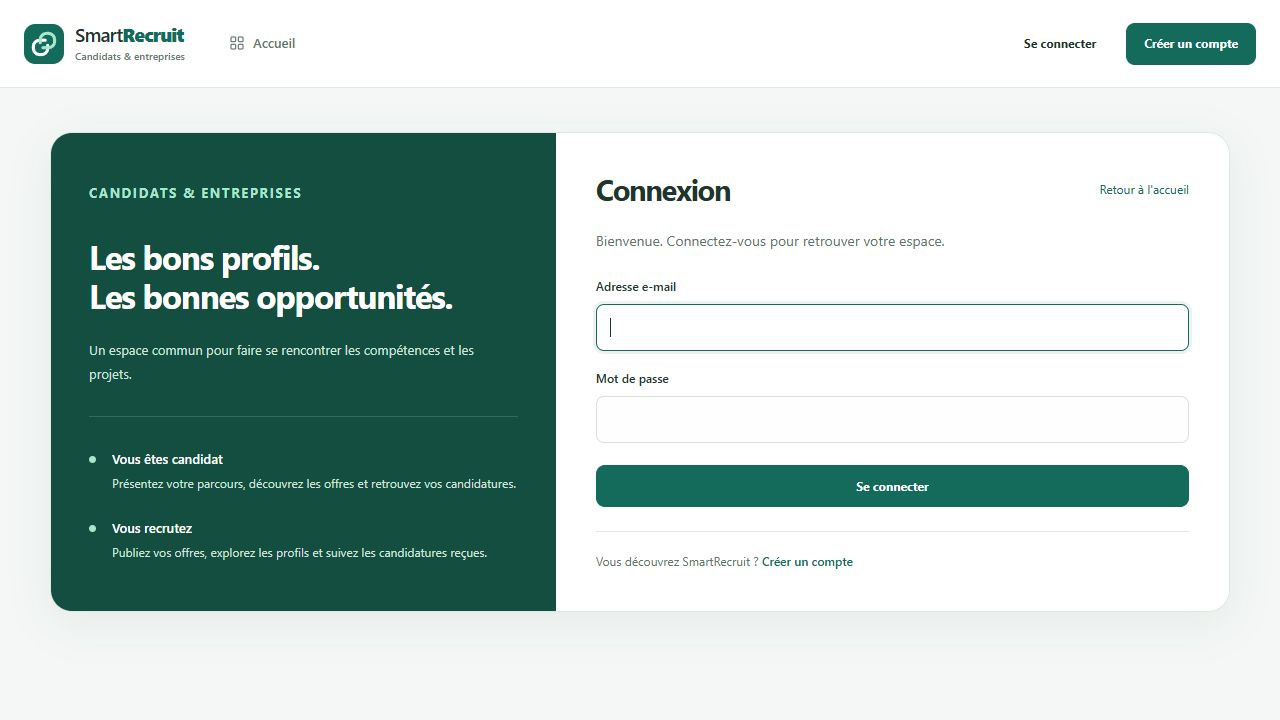
\includegraphics[width=.94\linewidth,height=.74\textwidth,keepaspectratio]{figures/screenshots/01-connexion.png}
\caption{Interface de connexion à SmartRecruit}
\label{fig:interface-01-connexion}\end{figure}
\end{landscape}

\begin{landscape}
\subsection{Choix du profil à l'inscription}
{\small\setstretch{1.05}
L'inscription commence par le choix du type de compte : candidat ou recruteur. Chaque option annonce le parcours associé et prépare le formulaire adapté. Le rôle d'administrateur ne fait pas partie des choix publics.\par}


\begin{figure}[H]\centering
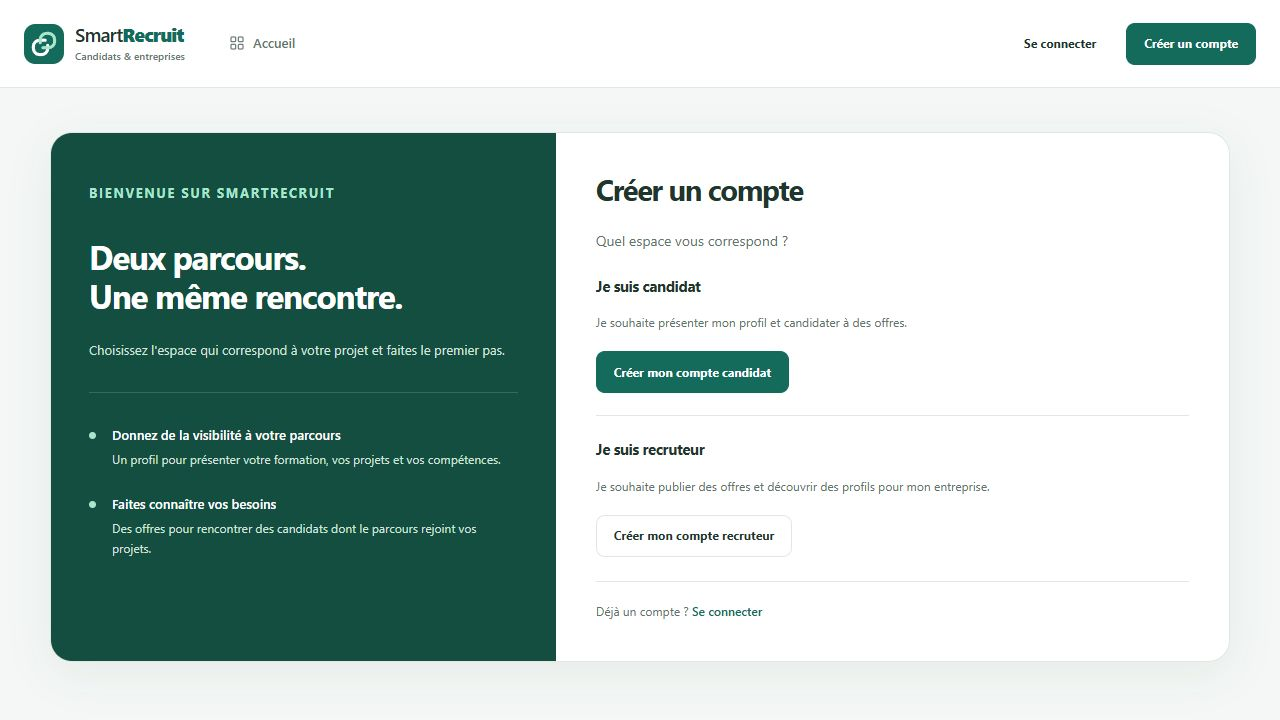
\includegraphics[width=.94\linewidth,height=.74\textwidth,keepaspectratio]{figures/screenshots/02-inscription.png}
\caption{Sélection du type de compte lors de l'inscription}
\label{fig:interface-02-inscription}\end{figure}
\end{landscape}

\begin{landscape}
\subsection{Espace candidat}
{\small\setstretch{1.05}
Le tableau de bord du candidat donne une vue d'ensemble de son profil et de son activité. Les accès aux offres et à la mise à jour du parcours facilitent les actions fréquentes. Le terme candidat employé à l'écran correspond au rôle étudiant du mémoire.\par}


\begin{figure}[H]\centering
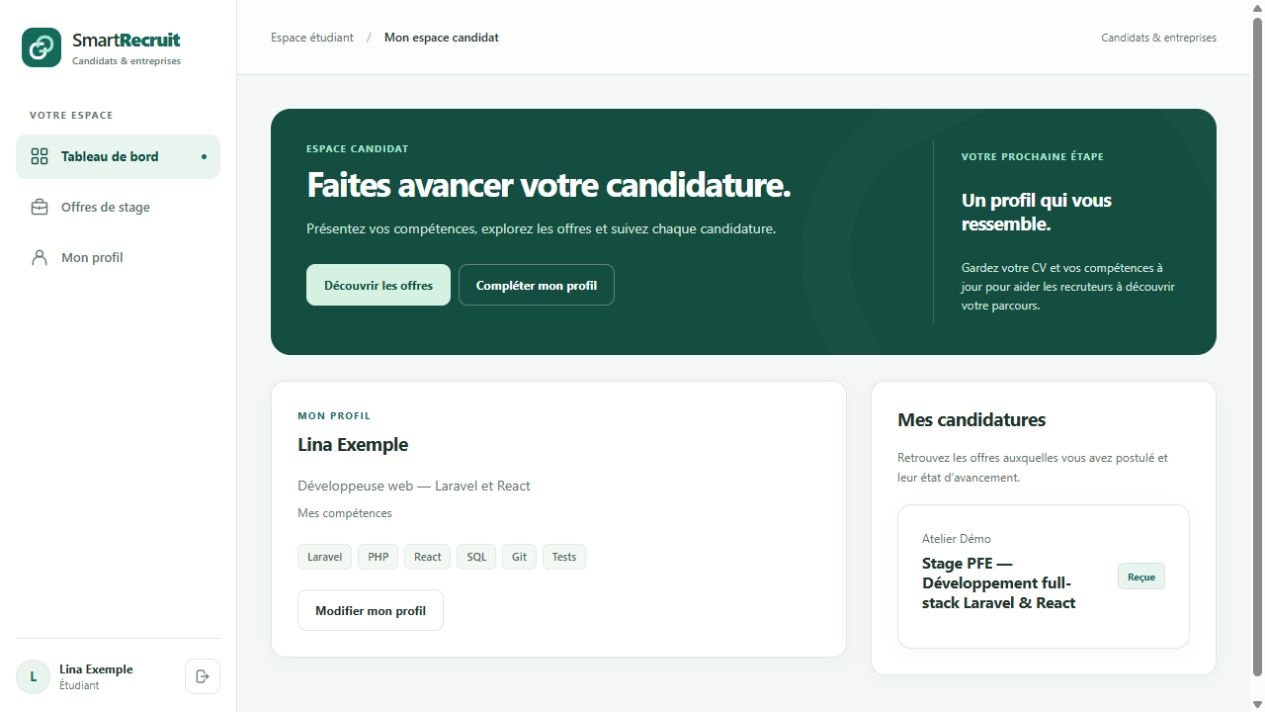
\includegraphics[width=.94\linewidth,height=.74\textwidth,keepaspectratio]{figures/screenshots/05-espace-etudiant.png}
\caption{Tableau de bord du candidat avec données de démonstration}
\label{fig:interface-05-espace-etudiant}\end{figure}
\end{landscape}

\begin{landscape}
\subsection{Profil et informations du CV}
{\small\setstretch{1.05}
La fiche rassemble les informations du parcours, les compétences et les éléments associés au CV. Cette restitution aide à relire les données utilisées lors du rapprochement avec une offre. La possibilité de corriger le profil complète l'extraction automatique décrite par la carte K04.\par}


\begin{figure}[H]\centering
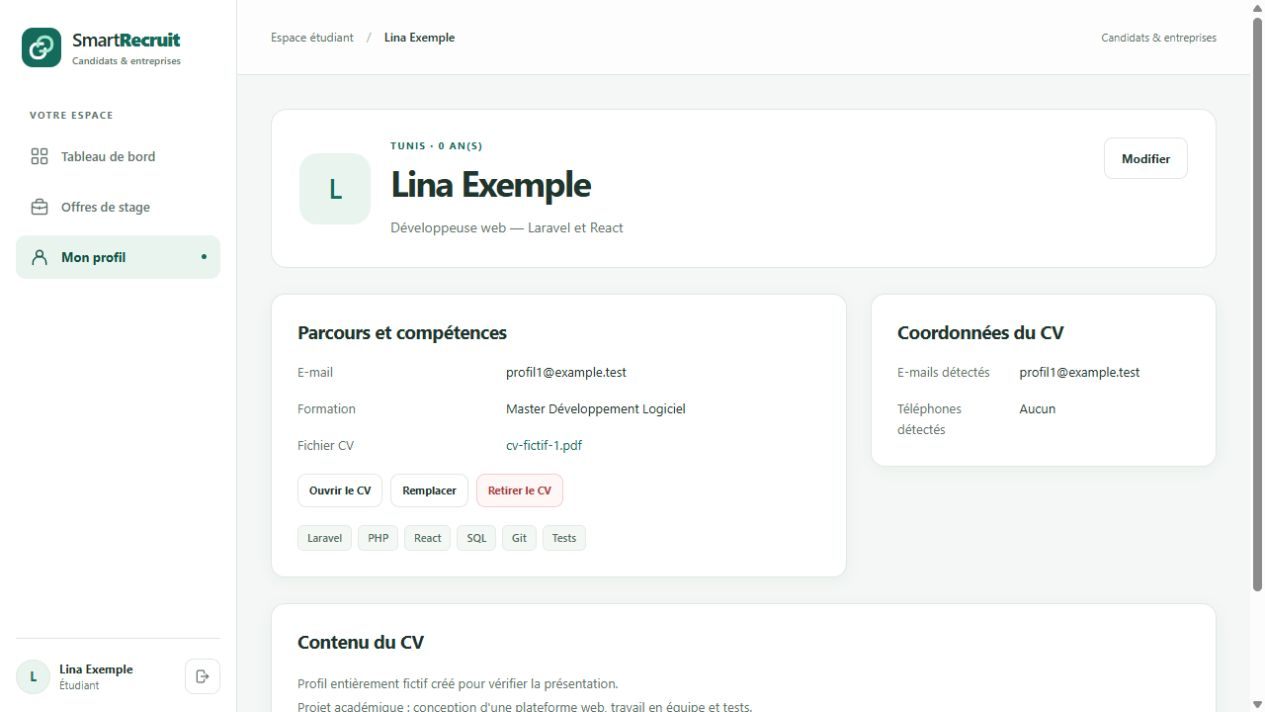
\includegraphics[width=.94\linewidth,height=.74\textwidth,keepaspectratio]{figures/screenshots/09-profil-etudiant.png}
\caption{Présentation du profil candidat et de ses compétences}
\label{fig:interface-09-profil-etudiant}\end{figure}
\end{landscape}

\begin{landscape}
\subsection{Catalogue des offres}
{\small\setstretch{1.05}
Les offres sont présentées avec les informations utiles à leur comparaison et un accès au détail. Des indicateurs de compatibilité et de suivi peuvent accompagner les résultats. Les valeurs visibles ici appartiennent au jeu illustratif ; elles ne mesurent pas la précision du moteur.\par}


\begin{figure}[H]\centering
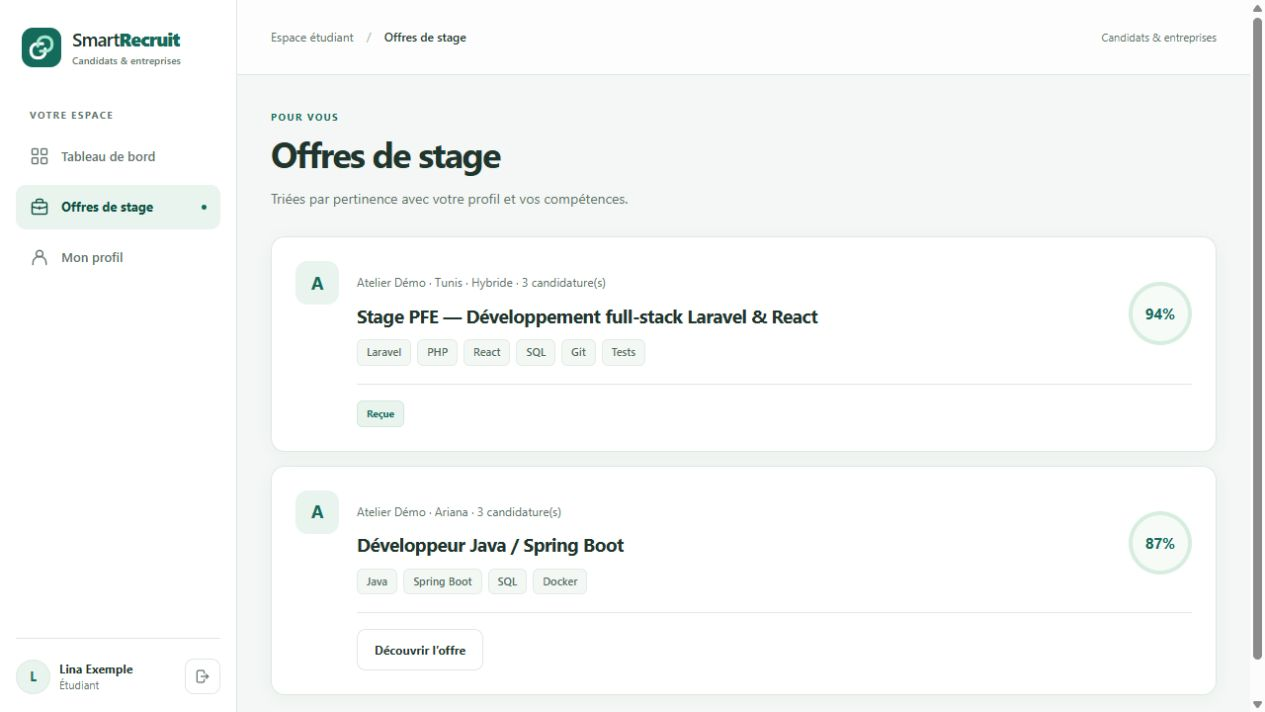
\includegraphics[width=.94\linewidth,height=.74\textwidth,keepaspectratio]{figures/screenshots/06-offres-etudiant.png}
\caption{Catalogue des offres dans l'espace candidat}
\label{fig:interface-06-offres-etudiant}\end{figure}
\end{landscape}

\begin{landscape}
\subsection{Détail d'une offre}
{\small\setstretch{1.05}
La page de détail expose la mission, les exigences et les informations de l'entreprise. Elle replace le rapprochement dans le contexte de l'offre et restitue la situation du candidat lorsqu'une candidature existe déjà. L'utilisateur peut ainsi comprendre le contenu du poste avant de poursuivre son suivi.\par}


\begin{figure}[H]\centering
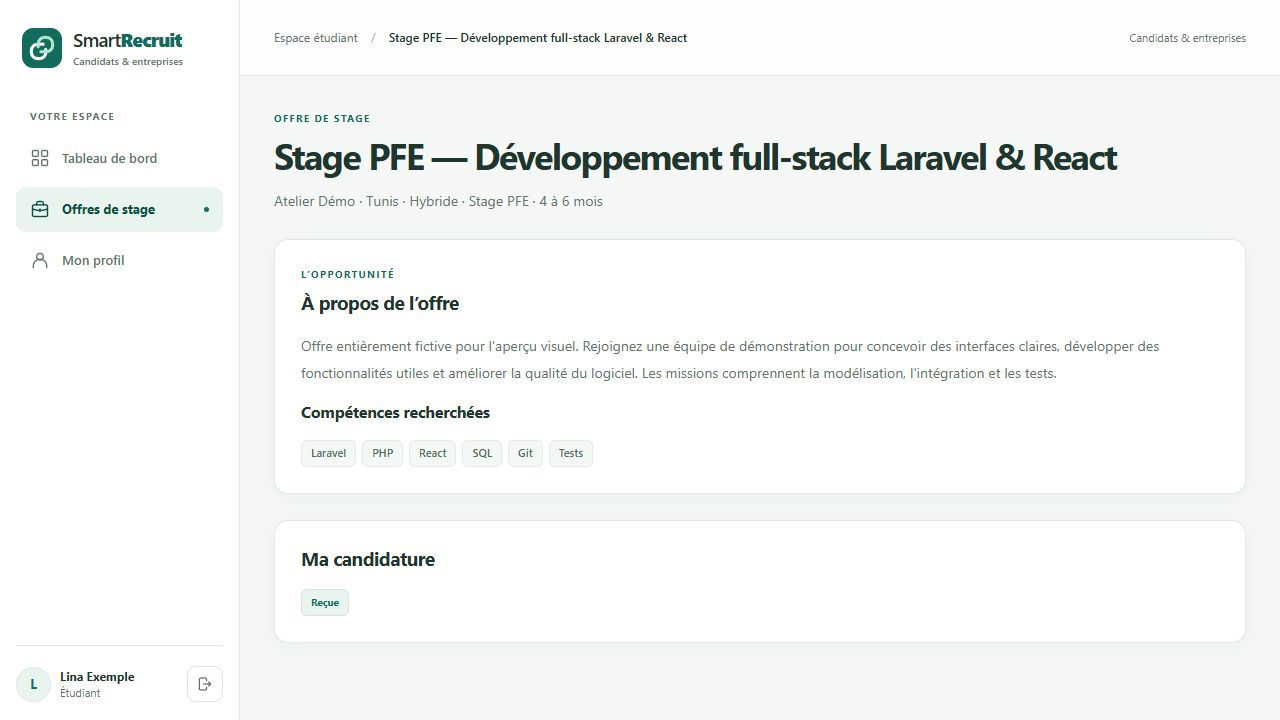
\includegraphics[width=.94\linewidth,height=.74\textwidth,keepaspectratio]{figures/screenshots/07-detail-offre.png}
\caption{Consultation d'une offre et de ses exigences}
\label{fig:interface-07-detail-offre}\end{figure}
\end{landscape}

\begin{landscape}
\subsection{Espace recruteur}
{\small\setstretch{1.05}
Le tableau de bord recruteur synthétise l'activité de ses offres et oriente vers leur gestion. Les filtres et les accès au vivier structurent le travail de consultation. Cette vue met en relation les cartes K05, K08 et K09, consacrées aux offres, aux décisions et au suivi.\par}


\begin{figure}[H]\centering
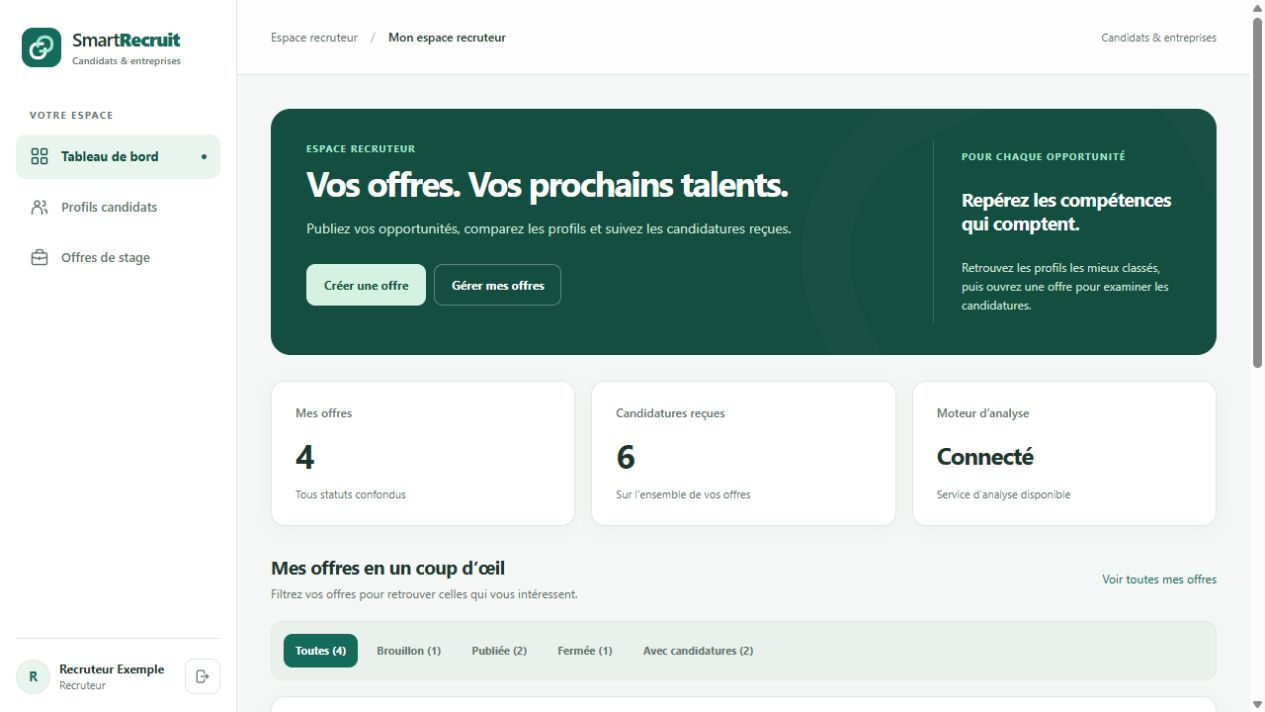
\includegraphics[width=.94\linewidth,height=.74\textwidth,keepaspectratio]{figures/screenshots/04-espace-recruteur.png}
\caption{Tableau de bord du recruteur}
\label{fig:interface-04-espace-recruteur}\end{figure}
\end{landscape}

\begin{landscape}
\subsection{Création d'une offre}
{\small\setstretch{1.05}
Le formulaire permet de décrire une opportunité et les compétences recherchées. La capture montre sa partie supérieure, avec les premiers champs nécessaires à la publication. Les informations saisies alimentent ensuite la consultation de l'offre et sa comparaison avec les profils.\par}


\begin{figure}[H]\centering
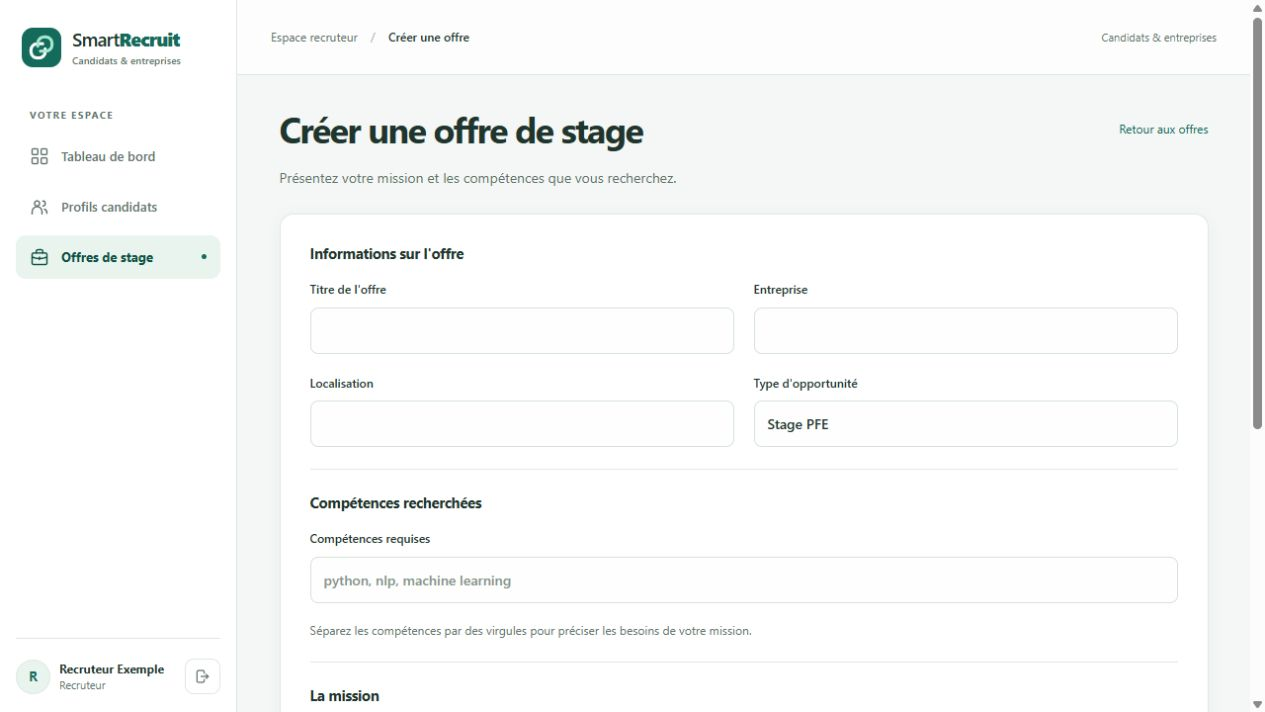
\includegraphics[width=.94\linewidth,height=.74\textwidth,keepaspectratio]{figures/screenshots/10-creation-offre.png}
\caption{Partie supérieure du formulaire de création d'une offre}
\label{fig:interface-10-creation-offre}\end{figure}
\end{landscape}

\begin{landscape}
\subsection{Vivier des candidats}
{\small\setstretch{1.05}
La liste des profils permet au recruteur de parcourir le vivier et d'accéder aux fiches détaillées. Les informations synthétiques facilitent une première lecture des parcours. La présence d'une personne dans ce vivier ne signifie pas qu'elle a postulé à une offre donnée.\par}


\begin{figure}[H]\centering
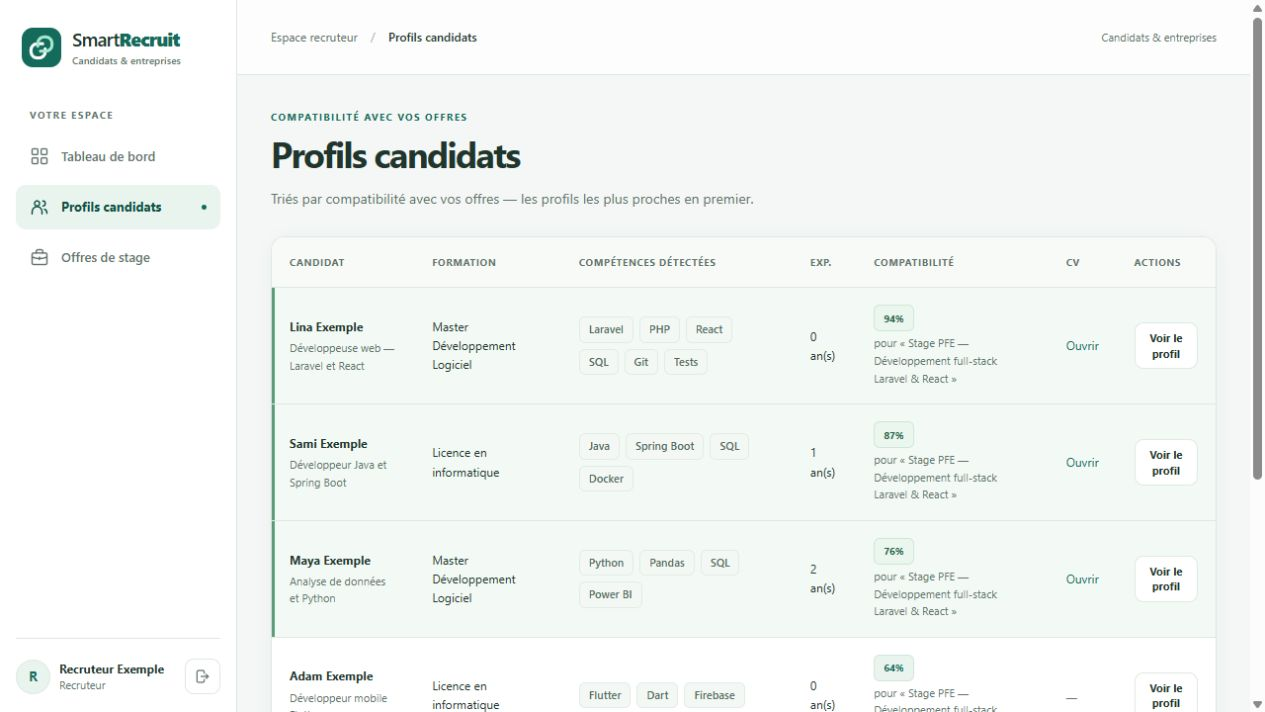
\includegraphics[width=.94\linewidth,height=.74\textwidth,keepaspectratio]{figures/screenshots/12-profils.png}
\caption{Consultation du vivier de profils par le recruteur}
\label{fig:interface-12-profils}\end{figure}
\end{landscape}

\begin{landscape}
\subsection{Classement pour une offre}
{\small\setstretch{1.05}
Le classement associe chaque profil à un score et à des éléments d'explication, notamment les compétences rapprochées ou manquantes. Les actions de décision concernent les candidatures existantes. La capture est centrée sur cette section de la page ; les scores sont des valeurs de démonstration.\par}


\begin{figure}[H]\centering
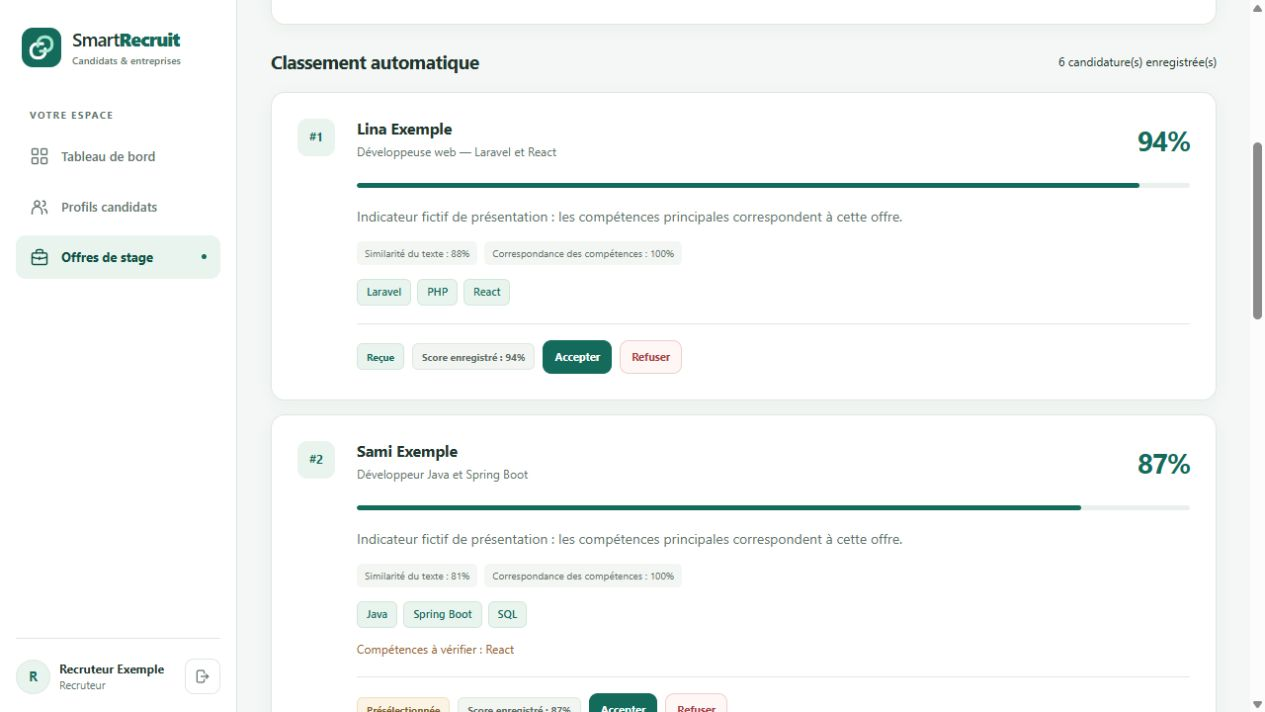
\includegraphics[width=.94\linewidth,height=.74\textwidth,keepaspectratio]{figures/screenshots/08-classement.png}
\caption{Section de classement des profils pour une offre}
\label{fig:interface-08-classement}\end{figure}
\end{landscape}

\begin{landscape}
\subsection{Supervision administrative}
{\small\setstretch{1.05}
L'espace administrateur fournit une vue transversale des comptes, des offres et des candidatures. Ses accès regroupent les fonctions de supervision et de gestion qui dépassent le périmètre d'un recruteur. Cette séparation rend visibles les responsabilités propres au troisième acteur UML.\par}


\begin{figure}[H]\centering
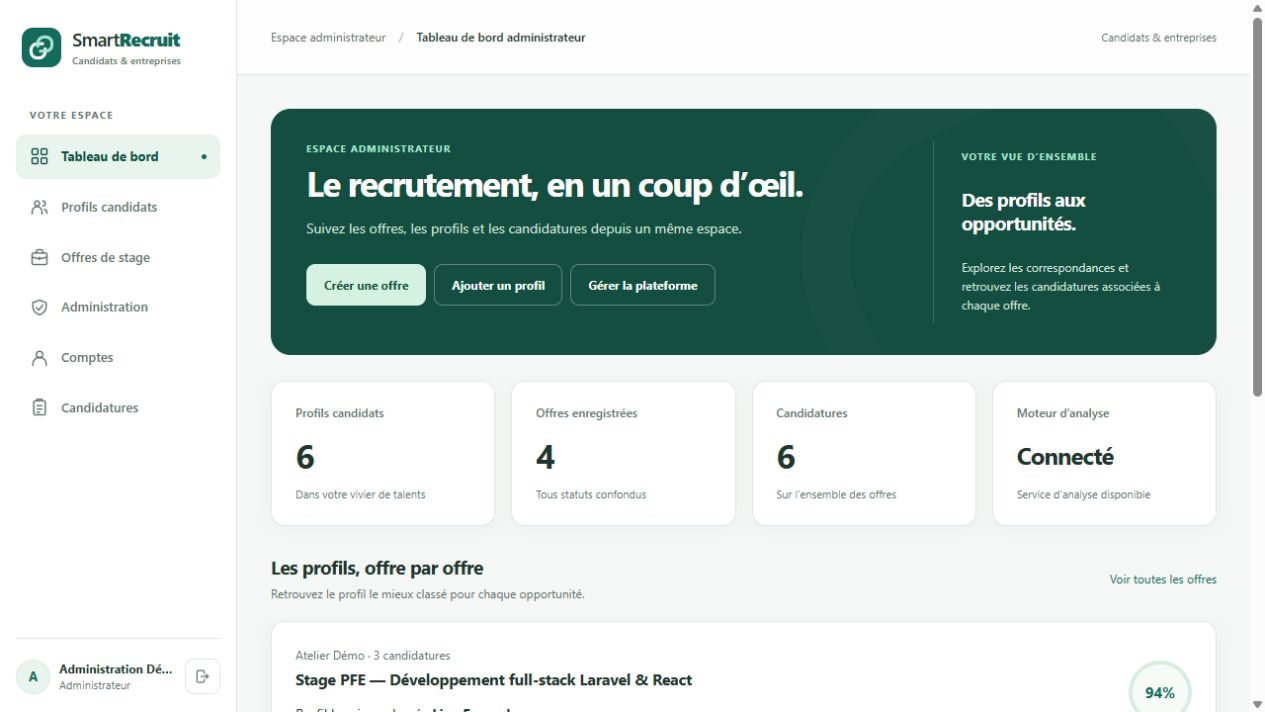
\includegraphics[width=.94\linewidth,height=.74\textwidth,keepaspectratio]{figures/screenshots/03-espace-administrateur.png}
\caption{Tableau de bord de l'administrateur}
\label{fig:interface-03-espace-administrateur}\end{figure}
\end{landscape}

\begin{landscape}
\subsection{Gestion des candidatures}
{\small\setstretch{1.05}
La liste administrative rassemble les candidatures, leur statut et les opérations de gestion. Les filtres permettent de retrouver les éléments actifs ou supprimés logiquement. Le statut métier et la présence dans la corbeille sont deux informations distinctes, conformément au diagramme d'états.\par}


\begin{figure}[H]\centering
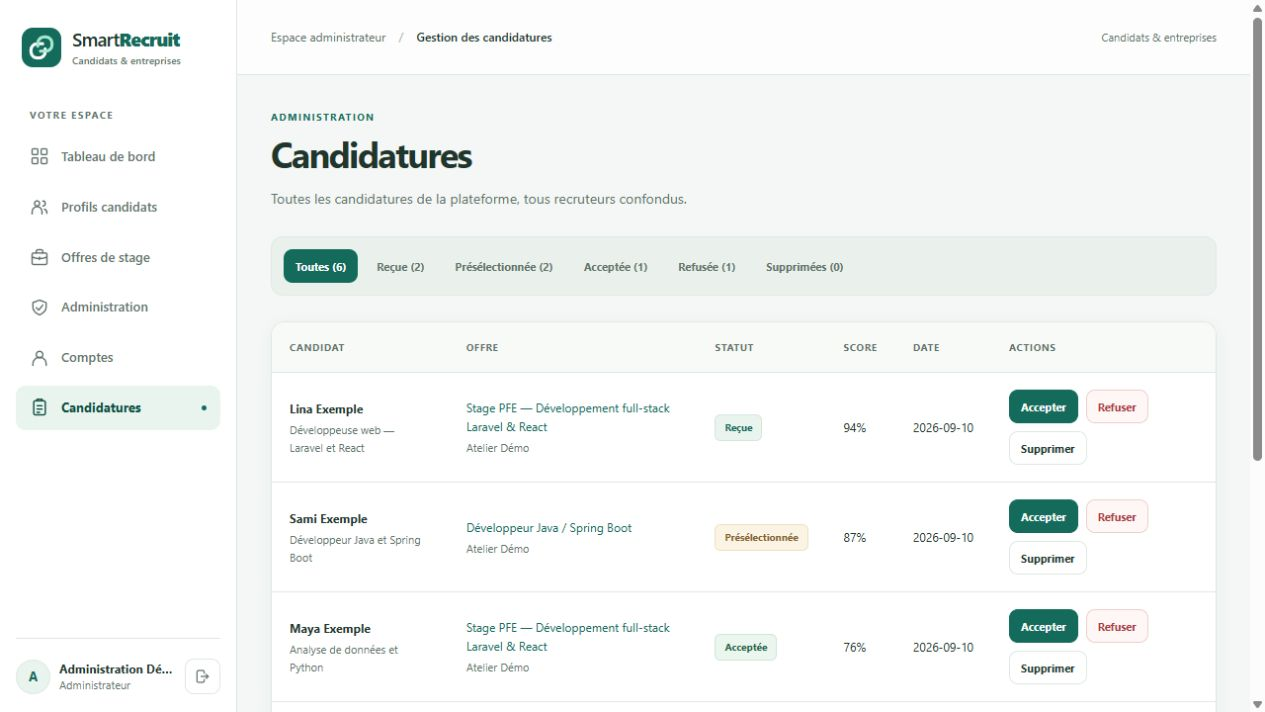
\includegraphics[width=.94\linewidth,height=.74\textwidth,keepaspectratio]{figures/screenshots/11-candidatures.png}
\caption{Suivi et gestion administrative des candidatures}
\label{fig:interface-11-candidatures}\end{figure}
\end{landscape}



\section{Intégration, limites et préparation du déploiement}
Le magasin actif est MySQL. La fonction \code{sr_store} échoue explicitement lorsque la base n'est pas disponible. L'ancien magasin JSON reste un artefact du dépôt et un support d'éléments de démonstration, sans être sélectionné comme persistance de substitution par les routes métier actuelles. Une chaîne de diagnostic ancienne ne suffit pas à établir l'existence d'un repli actif.

La séparation entre démonstration et usage réel demande toutefois un contrôle complémentaire : l'appel \code{all()} conserve un chemin d'initialisation ou de synchronisation de données de démonstration. Ce comportement explique pourquoi les captures du mémoire ont été produites sans ouvrir les routes métier contre la base existante. Avant un déploiement, l'initialisation doit devenir une opération explicite et maîtrisée.

Les paramètres de connexion, les secrets, les chemins de stockage et les ports relèvent de l'environnement. La présence de fichiers Docker ou d'un serveur local n'est pas une preuve de qualification d'une installation. La documentation Laravel et celle de Docker fournissent les mécanismes à configurer ; leur application doit ensuite être vérifiée sur un environnement isolé \cite{laravel-deployment,docker-compose}. Les fichiers CV nécessitent notamment une politique de conservation, des droits adaptés et un accès contrôlé.

La réalisation fournit ainsi une chaîne utilisateur cohérente, de la constitution du profil au suivi d'une candidature. Les captures rendent visibles les choix de présentation ; les contrats et le code expliquent leur fonctionnement. Le chapitre de validation précise la portée des preuves disponibles et les travaux à inscrire dans la réserve Kanban pour consolider cette base.

\chapter{Conception et fonctionnement du moteur de matching}
\label{chap:moteur}

Ce chapitre décrit les formules présentes dans le code examiné. Les exemples numériques sont des calculs illustratifs ou des sorties historiques explicitement identifiées dans le chapitre de validation. Les cartes K04 et K07 encadrent respectivement la qualité des données extraites et la restitution du score. Le label de provenance distant actuel est \code{python} ; le fichier historique du 11 septembre conserve l'ancien label \code{python-ai}.

\section{Organisation de la chaîne de traitement}

Le moteur transforme une offre et un profil étudiant en un ensemble d'indicateurs, puis en un score entier compris entre 0 et 100. Son fonctionnement repose sur quatre composants principaux : \path{app/Support/CvParser.php} prépare le contenu d'un CV ; \path{app/Support/SemanticMatcher.php} réalise le calcul local ; \path{app/Support/AiClient.php} communique avec le microservice ; \path{ai-service/app.py} expose l'extraction PDF et une seconde implémentation du score. L'orchestration des appels se trouve dans \path{routes/web.php}.

La figure~\ref{fig:matching-pipeline} présente cette chaîne. Le fichier constitue une source possible du profil, auquel s'ajoutent les champs saisis. Le rapprochement exploite ensuite deux représentations complémentaires : des ensembles de compétences et des vecteurs lexicaux. Les catégories sont déduites des compétences reconnues. Aucun modèle neuronal n'est chargé dans ce parcours et aucun apprentissage de coefficients n'est réalisé à l'exécution.

\begin{figure}[H]
\centering
\begingroup\singlespacing
\begin{tikzpicture}[node distance=9mm]
\node[block,text width=11cm] (in) {\textbf{Données d'entrée}\\Texte de l'offre, texte du CV, compétences explicites};
\node[block,text width=11cm,below=of in] (norm) {\textbf{Préparation}\\Normalisation, extraction de compétences, remplacement d'alias};
\node[block,text width=3.1cm,below=13mm of norm] (cos) {TF-IDF sur la paire\\Similarité cosinus};
\node[block,text width=3.1cm,left=7mm of cos] (skill) {Couverture des\\compétences requises};
\node[block,text width=3.1cm,right=7mm of cos] (cat) {Couverture des\\catégories techniques};
\node[block,text width=11cm,below=15mm of cos] (score) {\textbf{Combinaison pondérée et arrondi}\\PHP : bonus d'expérience ; Python : pondérations différentes};
\node[block,text width=11cm,below=of score] (out) {\textbf{Résultat de matching}\\Score 0--100, compétences trouvées et manquantes, source};
\draw[arr](in)--(norm);
\draw[arr](norm)--(cos);
\draw[arr](norm.south -| skill.north)--(skill);
\draw[arr](norm.south -| cat.north)--(cat);
\draw[arr](cos)--(score);
\draw[arr](skill.south)--(score.north -| skill.south);
\draw[arr](cat.south)--(score.north -| cat.south);
\draw[arr](score)--(out);
\end{tikzpicture}

\endgroup

\caption{Chaîne de préparation des données et de calcul du matching dans SmartRecruit}
\label{fig:matching-pipeline}
\end{figure}

Le texte de l'offre concatène son titre, sa description et les compétences requises. Celui du candidat concatène son intitulé de profil, sa formation, le texte de son CV et ses compétences. Cette composition est importante : une compétence présente à la fois dans le CV et dans un champ structuré peut apparaître plusieurs fois dans le texte. Les ensembles de compétences sont dédupliqués, mais les fréquences lexicales conservent ces répétitions. Les champs structurés influencent donc les deux branches du calcul.

\section{Extraction et préparation du CV}

\subsection{Sources textuelles et extraction PDF}

La méthode \code{CvParser::parse} accepte un fichier optionnel et un texte manuel. Lorsqu'un fichier est fourni, elle tente d'en extraire le contenu, puis concatène le résultat avec le texte manuel. Le texte saisi complète ainsi le contenu extrait ; il ne le remplace pas automatiquement. La méthode renvoie notamment le texte final, les compétences, une estimation de l'expérience, une formation détectée et des métadonnées de contact.

Pour un fichier portant l'extension PDF, le parseur appelle d'abord \code{AiClient::parseCv} lorsque le client est disponible. L'appel transmet le fichier en multipart au point d'accès \path{/parse-cv}, avec un délai maximal configuré de six secondes. Côté Python, un fichier temporaire est créé, alimenté puis supprimé dans un bloc \code{finally}. Le mécanisme d'accès aux fichiers reçus correspond au modèle décrit par Flask pour les téléversements \cite{flask-docs}.

L'extraction Python tente d'abord \code{pdfminer.high_level.extract_text}. En cas d'exception, elle essaie l'interface PyPDF2 présente dans le code. Si ces tentatives échouent, elle lit les octets et les décode en Latin-1. Ce dernier comportement est une limite : obtenir une chaîne de caractères à partir d'un PDF ne signifie pas avoir extrait son contenu rédactionnel. De plus, lorsque pdfminer retourne une chaîne vide sans exception, la fonction renvoie directement cette chaîne et ne poursuit pas la tentative PyPDF2.

En l'absence de résultat Python non vide, PHP utilise une extraction locale. Les fichiers TXT, Markdown et CSV sont lus comme du texte brut. Pour un PDF, une expression régulière retire certains délimiteurs de parenthèses, puis un filtrage conserve des lettres, chiffres et caractères particuliers. Cette procédure ne décompresse pas les flux PDF et ne reconstruit pas leur structure. Aucune étape de reconnaissance optique de caractères n'est implémentée pour les pages numérisées sous forme d'images.

Le champ \code{extraction_unreliable} devient vrai lorsqu'un fichier a été fourni, que le texte extrait contient moins de 40 caractères et qu'aucun texte manuel ne compense cette situation. Cette garde rend visible un échec simple, mais sa portée reste limitée. Un contenu technique de plus de 40 caractères peut franchir le seuil sans être un CV exploitable. La correction proposée consiste à retourner un statut d'extraction distinct du texte, plutôt qu'à interpréter uniquement sa longueur ; elle ne fait pas partie du code étudié.

\subsection{Compétences, formation et expérience}

Les compétences et les coordonnées sont recherchées dans le texte final. Les adresses électroniques et les numéros de téléphone sont extraits par expressions régulières, sans validation de leur caractère opérationnel. La formation est déterminée par la première correspondance dans une liste ordonnée : doctorat, master, mastère, ingénieur, licence, bachelor et BTS. Ce mécanisme ne reconstitue pas un parcours académique. Il peut retenir un diplôme mentionné comme objectif ou dans une autre partie du document.

L'expérience est obtenue en recherchant un entier suivi d'une expression telle que \emph{ans}, \emph{années} ou \emph{year(s)}. La présence du mot \emph{expérience} est facultative dans l'expression régulière. La méthode retient le maximum des nombres détectés et retourne zéro en l'absence de correspondance. Elle ne calcule pas la durée d'intervalles datés, ne cumule pas des stages et ne gère pas leurs chevauchements.

Cette règle explique qu'une mention d'âge ou de durée d'études puisse devenir une expérience professionnelle. L'incidence est directe puisque cette estimation peut alimenter le profil et le bonus du moteur PHP. Il conviendrait de conserver la provenance de la valeur, de limiter l'inférence aux formulations explicitement professionnelles et de permettre sa vérification. Les sondes ciblées du chapitre~\ref{chap:validation} illustrent ce problème ; elles ne mesurent pas une précision globale d'extraction sur un corpus de CV.

\section{Normalisation, alias et catégories}

\subsection{Traitement lexical effectivement implémenté}

Le moteur PHP transforme le texte en minuscules avec \code{mb_strtolower}, puis tente une translittération vers ASCII avec \code{iconv}. Il remplace ensuite par des espaces les caractères hors de l'ensemble formé des lettres ASCII, chiffres, signes plus, dièse et point. Les espaces successifs sont réduits. Le moteur Python applique une mise en minuscules et un filtrage comparable, mais ne réalise pas la translittération préalable : une lettre accentuée est éliminée par le filtre ASCII. La normalisation du français ne peut donc pas être considérée comme identique dans les deux langages.

L'extraction des compétences recherche chaque alias normalisé avec un espace avant et après. Cette précaution évite certaines correspondances au milieu d'un mot. Cependant, le point est conservé par la normalisation : \emph{Python.} ne correspond pas à l'alias \emph{python} entouré d'espaces. La conservation de caractères utiles aux noms techniques nécessite ainsi un traitement plus précis de la ponctuation terminale.

La tokenisation constitue une opération différente. Après normalisation, les alias sont remplacés successivement par leur nom canonique ; les espaces internes de ce nom deviennent des underscores. Le texte est découpé sur les espaces, puis les tokens de longueur inférieure ou égale à deux et les mots vides français ou anglais sont supprimés. Les substitutions n'utilisent pas les limites de mots de l'extracteur. Leur ordre peut modifier un alias avant qu'un alias plus long soit examiné : \emph{Spring Boot} devient ainsi \emph{java boot}, tandis que \emph{React.js} peut produire \emph{react.javascript}.

\subsection{Rôle du dictionnaire et de la taxonomie}

Le dictionnaire PHP défini dans \path{config/smart_recruit.php} contient 21 compétences canoniques. Celui de Python en contient 16. Les entrées Angular, NoSQL, cloud, mobile et sécurité sont présentes uniquement côté PHP. Certaines correspondances expriment une famille technique : Laravel et Symfony sont associés à PHP ; Spring et Spring Boot à Java ; pandas et NumPy à l'analyse de données. Ce sont des règles de rapprochement retenues dans le prototype, et non des équivalences exhaustives entre niveaux de maîtrise.

La taxonomie associe ensuite chaque compétence connue à une catégorie : Java, PHP et Python au développement backend ; React et Vue au frontend ; SQL aux données ; DevOps à l'infrastructure. Les catégories sont dédupliquées. Posséder plusieurs compétences backend n'apporte donc qu'une catégorie à ce niveau. Cette réduction permet de valoriser une proximité de domaine même sans identité de technologie, mais elle peut aussi rapprocher des connaissances professionnelles très différentes.

Le traitement des compétences explicitement saisies diverge également. PHP les canonise : pour chaque chaîne, il retient la première compétence détectée ou, à défaut, sa forme normalisée. Python conserve les valeurs reçues et les réunit aux compétences extraites du texte, sans canonisation préalable. Une valeur explicite \emph{Laravel} peut ainsi coexister avec la compétence extraite \emph{php}. Cette duplication conceptuelle modifie le dénominateur de la couverture et peut créer un manque artificiel.

\section{Définition des composantes mathématiques}

\subsection{Couverture des compétences et des catégories}

Soient $R$ l'ensemble des compétences considérées comme requises et $P$ l'ensemble des compétences du profil, après les traitements propres au moteur utilisé. Les compétences communes sont $M=R\cap P$ et les manques sont $D=R\setminus P$. La couverture des compétences est définie par :
\begin{equation}
C(R,P)=
\begin{cases}
\dfrac{|R\cap P|}{|R|}, & \text{si } |R|>0,\\[4pt]
0, & \text{sinon}.
\end{cases}
\label{eq:couverture-competences}
\end{equation}

Cette mesure est orientée par le besoin : des compétences supplémentaires du candidat n'augmentent pas directement $C$, mais des compétences requises supplémentaires peuvent le diminuer. Toutes les compétences ont le même poids. Le code ne distingue pas une obligation d'une préférence lorsqu'il extrait les compétences de la description de l'offre. La mention d'une technologie dans une phrase contextuelle peut donc enrichir $R$ comme une exigence explicite.

En notant $\Gamma(A)$ l'ensemble des catégories connues associées aux compétences de $A$, la couverture sémantique du code est :
\begin{equation}
K(R,P)=
\begin{cases}
\dfrac{|\Gamma(R)\cap\Gamma(P)|}{|\Gamma(R)|}, & \text{si } |\Gamma(R)|>0,\\[4pt]
0, & \text{sinon}.
\end{cases}
\label{eq:couverture-categories}
\end{equation}

Les compétences absentes de la taxonomie ne participent pas à $\Gamma$. Si l'offre n'exige que Java et que le profil ne mentionne que PHP, les catégories backend coïncident : $K=1$ tandis que $C=0$. Ce résultat exprime le choix de granularité de la taxonomie. Il ne prouve pas que le candidat satisfait l'exigence Java.

\subsection{TF-IDF calculé sur une paire de documents}

Soient $d_o$ et $d_c$ les listes de tokens de l'offre et du candidat. Le corpus du calcul est toujours la paire $\mathcal{D}=(d_o,d_c)$, avec deux documents comptés séparément même si leurs textes sont identiques. Pour un terme $t$, $n(t,d)$ désigne son nombre d'occurrences et $|d|$ le nombre de tokens du document. Les deux implémentations utilisent :
\begin{align}
\operatorname{tf}(t,d) &= \frac{n(t,d)}{\max(|d|,1)},\\
\operatorname{df}(t,\mathcal{D}) &=
\sum_{d\in\mathcal{D}} \mathbf{1}_{\{t\in d\}},\\
\operatorname{idf}(t,\mathcal{D}) &=
\ln\left(\frac{1+2}{1+\operatorname{df}(t,\mathcal{D})}\right)+1,\\
v_d(t) &= \operatorname{tf}(t,d)\operatorname{idf}(t,\mathcal{D}).
\label{eq:tfidf-projet}
\end{align}

La constante ajoutée évite une pondération nulle pour un terme commun. Un terme présent dans les deux documents possède une IDF de $1$ ; un terme présent dans un seul document possède une IDF de $1+\ln(3/2)$, soit environ $1{,}405465$. Ces deux valeurs épuisent les cas pour les termes effectivement présents. Le moteur n'estime donc pas la rareté d'une technologie dans une population de candidats.

Le cosinus est calculé sur l'union des termes des deux documents :
\begin{equation}
T(d_o,d_c)=
\begin{cases}
\dfrac{\sum_t v_{d_o}(t)v_{d_c}(t)}
{\sqrt{\sum_t v_{d_o}(t)^2}\sqrt{\sum_t v_{d_c}(t)^2}},
& \text{si les deux normes sont non nulles},\\[7pt]
0, & \text{sinon}.
\end{cases}
\label{eq:cosinus-projet}
\end{equation}

La division par la longueur du document dans TF multiplie chaque vecteur par un facteur uniforme, qui s'annule dans le cosinus lorsque les normes sont non nulles. Elle ne supprime pas l'effet du vocabulaire supplémentaire : de nouveaux termes modifient la direction du vecteur. De même, répéter sélectivement une compétence peut modifier les fréquences relatives. Le calcul conserve donc une sensibilité à la rédaction du profil.

\section{Formules finales PHP et Python}

En notant $e$ la valeur numérique de \code{experience_years}, avec zéro par défaut, le bonus PHP est défini par :
\begin{equation}
B(e)=0{,}05\min\left(\frac{e}{5},1\right).
\label{eq:bonus-experience}
\end{equation}
Il atteint cinq points à partir de cinq ans pour une entrée non négative. Le code ne borne pas séparément ce bonus vers le bas ; la borne générale du score s'applique ensuite. Avec $\operatorname{clip}(x)=\max(0,\min(100,x))$, les formules exactes sont :
\begin{align}
S_{\mathrm{PHP}} &= \operatorname{clip}\!\left(
\operatorname{arrondi}_{\mathrm{PHP}}\!\left[
100\left(0{,}55C+0{,}30T+0{,}10K+B(e)\right)\right]\right),
\label{eq:score-php}\\
S_{\mathrm{Python}} &= \operatorname{clip}\!\left(
\operatorname{arrondi}_{\mathrm{Python}}\!\left[
100\left(0{,}58C+0{,}32T+0{,}10K\right)\right]\right).
\label{eq:score-python}
\end{align}

Les arrondis désignent les fonctions natives appelées par chaque langage, puis la conversion en entier. Python emploie l'arrondi au pair pour les valeurs exactement à mi-chemin ; PHP utilise par défaut un arrondi des demis en s'éloignant de zéro. Une recherche d'équivalence doit donc couvrir également les valeurs frontières et la représentation flottante, au-delà de l'égalité des coefficients.

Les coefficients sont fixés dans le code. Ils ne résultent pas d'une optimisation sur un corpus annoté. Avec $C=T=K=1$ et $e=0$, PHP retourne 95 tandis que Python retourne 100. En l'absence de toute compétence requise reconnue ou déclarée, $C$ vaut zéro ; lorsque la taxonomie requise est vide, $K$ vaut également zéro. Même des textes identiques peuvent alors obtenir un score limité par les seuls coefficients du cosinus et, en PHP, de l'expérience.

PHP ajoute une explication selon des seuils de 80 et 60, puis selon la présence de compétences communes ou manquantes. Ces textes sont des descriptions de classes de score, pas des justifications causales détaillées. Python ne renvoie pas ce champ. Les deux moteurs utilisent pourtant le même identifiant d'algorithme, \code{tf-idf-cosine+semantic-skill-taxonomy}, ce qui ne suffit pas à identifier précisément les règles exécutées.

\section{Exemple numérique reproductible}

Considérons une offre dont le texte est \emph{java react} et un profil dont le texte est \emph{java sql}. Les autres champs textuels et les listes explicites sont vides ; l'expérience vaut deux ans pour le calcul PHP. Les tokens restent inchangés. Les compétences requises sont $R=\{\text{java},\text{react}\}$ et celles du profil $P=\{\text{java},\text{sql}\}$. Ainsi, $M=\{\text{java}\}$, $D=\{\text{react}\}$ et $C=1/2$.

Les catégories de l'offre sont backend et frontend ; celles du profil sont backend et data. Leur intersection contient une catégorie sur deux, d'où $K=1/2$. Posons $a=1+\ln(3/2)$. Dans l'ordre de dimensions Java, React, SQL, les vecteurs sont :
\begin{equation}
v_o=\left(\frac{1}{2},\frac{a}{2},0\right),
\qquad
v_c=\left(\frac{1}{2},0,\frac{a}{2}\right).
\end{equation}
Le produit scalaire vaut $1/4$ et chaque norme vaut $\sqrt{1+a^2}/2$. Il en résulte :
\begin{equation}
T=\frac{1}{1+a^2}\simeq 0{,}336096927.
\end{equation}

Les contributions sont détaillées dans le tableau~\ref{tab:exemple-score}. Les valeurs intermédiaires gardent ici plusieurs décimales pour rendre le calcul vérifiable ; elles ne constituent pas une mesure expérimentale de pertinence.

\begin{table}[htbp]
\centering
\caption{Contributions en points pour l'exemple Java, React et SQL}
\label{tab:exemple-score}
\begin{tabular}{@{}lrr@{}}
\toprule
Composante & PHP & Python \\
\midrule
Couverture des compétences & $27{,}50$ & $29{,}00$ \\
Similarité textuelle & $10{,}082908$ & $10{,}755102$ \\
Couverture des catégories & $5{,}00$ & $5{,}00$ \\
Expérience de deux ans & $2{,}00$ & $0{,}00$ \\
\midrule
Total avant arrondi & $44{,}582908$ & $44{,}755102$ \\
Score retourné & $45$ & $45$ \\
\bottomrule
\end{tabular}
\end{table}

Les deux moteurs donnent donc le même entier dans cet exemple malgré des calculs différents. Ils retournent une similarité textuelle arrondie à 34 et une couverture des catégories de 50. La compétence commune est Java et la compétence manquante est React. Cette égalité ponctuelle montre pourquoi quelques exemples positifs ne suffisent pas à démontrer la parité de deux implémentations.

\section{Contrat HTTP et mécanisme de repli}

Le service expose trois points d'accès. \path{GET /health} retourne un statut et l'identifiant de l'algorithme. \path{POST /match} reçoit \code{offer_text}, \code{cv_text}, \code{required_skills} et \code{candidate_skills}, puis retourne le score, les compétences communes et manquantes, les deux indicateurs et la source. \path{POST /parse-cv} reçoit un champ fichier et retourne du texte, des adresses électroniques et des compétences. L'expérience ne figure pas dans la requête de matching Python.

Le contrôle de disponibilité est réalisé avant une série de comparaisons. Pour chaque paire, la fonction \code{sr_match} calcule d'abord le résultat PHP. Lorsque le service est déclaré disponible, elle lui demande un résultat et remplace certains champs si la réponse contient un score. Le délai configuré pour les appels JSON de \code{AiClient} est de 0,4 seconde. Une absence de réponse exploitable conserve le résultat local. Cette organisation protège la disponibilité fonctionnelle, mais ajoute un calcul local même lorsqu'un score Python sera ensuite retenu.

La validation du contrat reste partielle. Le client JSON accepte une réponse décodée en tableau sans contrôler explicitement le statut HTTP. L'orchestrateur exige la présence du score mais ne vérifie pas l'ensemble du schéma. Le point d'accès Python accepte aussi les données sans validation systématique des types. Une requête contenant un nombre à la place d'un texte peut donc déclencher une exception. Ces observations motivent un schéma d'entrée et de sortie commun et des réponses d'erreur contrôlées, proposés comme améliorations.

Le démarrage Python prévoit plusieurs modes. Lorsque Flask et Waitress sont disponibles, Waitress sert l'application WSGI. Sans Waitress, le serveur intégré de Flask est utilisé. Sans Flask, un serveur de secours fondé sur la bibliothèque standard expose encore la santé et le matching, mais retourne 501 pour l'extraction multipart PDF. Un statut de santé positif ne garantit donc pas à lui seul la disponibilité de toutes les capacités du service.

Les classements sont construits par comparaisons synchrones. Pour $n$ profils et $m$ offres, la recommandation du meilleur rapprochement de chaque étudiant peut effectuer $n\times m$ calculs et autant d'appels Python. Il s'agit d'une propriété des boucles présentes, pas d'une mesure de latence. Un traitement par lots ou une mise en cache exigerait une clé tenant compte des textes, compétences et versions du moteur pour éviter de réutiliser un score devenu obsolète.

\section{Divergences constatées et trajectoire de correction}

Les différences décrites ont des conséquences observables. Avec des textes identiques \emph{angular aws mongodb}, sans listes explicites ni expérience, le moteur PHP reconnaît trois compétences et retourne 95 ; Python n'en reconnaît aucune et retourne 32. Ce cas déterministe, repris au chapitre~\ref{chap:validation}, démontre une divergence de contrat métier. Il ne permet pas de conclure à une supériorité générale du moteur PHP sur un jeu de recrutement.

L'intégration présente une autre incohérence : lors du remplacement du résultat PHP par celui de Python, l'explication PHP est conservée. Elle peut donc décrire une forte compatibilité alors que le score final est faible. La correction devrait produire l'explication à partir des indicateurs finalement retenus, ou inclure une explication vérifiée dans le contrat commun. Elle devrait aussi identifier la version du dictionnaire et de la formule, car la seule source \code{local-php} ou \code{python} est insuffisante pour reproduire durablement un résultat.

Une première évolution consisterait à externaliser le dictionnaire, la taxonomie, les coefficients et les règles d'arrondi dans une spécification partagée. Les deux moteurs devraient utiliser la même normalisation des compétences explicites et des alias. Les substitutions devraient respecter les limites de mots et traiter les expressions longues avant leurs fragments. Cette évolution suppose des tests de parité sur des entrées identiques, notamment pour les accents, la ponctuation et les noms techniques composés.

Une seconde évolution concernerait la qualité des données. Le parseur devrait distinguer texte extrait, contenu illisible et saisie manuelle ; les métadonnées inférées devraient conserver leur provenance. Les erreurs du service devraient être observables sans journaliser les CV. Enfin, la cohérence fonctionnelle du repli devrait être testée indépendamment de sa disponibilité réseau : un service de secours est utile seulement si son résultat garde une interprétation maîtrisée.

Ces propositions décrivent un travail restant à réaliser. Elles précèdent logiquement l'ajout d'un modèle appris, car une vectorisation plus élaborée ne corrigerait pas un PDF mal extrait ni des champs incohérents. Une expérimentation future pourrait comparer le moteur stabilisé à des représentations de phrases, mais devrait conserver des entrées, annotations et critères communs. Dans l'état étudié, la contribution est un calcul heuristique explicable dont les formules, conditions de fonctionnement et limites peuvent être examinées et reproduites.

\chapter{Validation, maîtrise du flux Kanban et perspectives}
\label{chap:validation}

\section{Périmètre et statut des résultats}

L'évaluation de SmartRecruit poursuit trois objectifs : vérifier que le code disponible constitue un ensemble techniquement cohérent, examiner quelques comportements déterminants et définir les preuves nécessaires avant une utilisation réelle. Elle porte sur le prototype décrit au chapitre~\ref{chap:realisation}. Les sondes chiffrées et contrôles techniques ci-dessous proviennent de l'analyse des 10 et 11 septembre 2026. La révision du 13 septembre relit le code et ajoute les preuves de rendu des interfaces, sans rejouer la campagne historique ni qualifier les parcours MySQL. Ils ne sont pas attribués rétrospectivement au stage de Rahma Amiri chez Best Solutions, qui s'est déroulé du 2 mars au 2 juillet 2026. Cette précision chronologique distingue les réalisations du projet des vérifications complémentaires effectuées pour documenter le mémoire.

Les résultats ne constituent ni une qualification de production ni une étude statistique de la qualité du recrutement. Les vérifications locales n'ont pas exécuté de campagne de charge, d'étude d'utilisabilité, de tests avec des recruteurs, de déploiement Docker ou de scénario complet sur la base métier existante. Aucun taux de précision global ni aucune latence de service ne sont donc annoncés. Les chiffres rapportés correspondent exclusivement aux sorties des contrôles identifiés. Les corrections décrites dans ce chapitre sont proposées ; leur présentation ne signifie pas qu'elles ont été appliquées au code.

\section{Méthodologie de vérification}

\subsection{Trois niveaux de preuve}

Le premier niveau consiste à lire le code et les configurations : routes, middleware, formulaires, magasins de données, parseurs et scripts de lancement. Il permet d'établir l'existence d'un contrôle ou d'un chemin d'exécution, mais pas de prouver le succès d'une transaction sur un serveur réel. Le deuxième niveau repose sur des exécutions locales ciblées : analyse syntaxique PHP, inspection des routes, vérification des dépendances et sondes portant sur les fonctions de calcul ou les frontières HTTP. Le troisième niveau rassemble les essais proposés, qui nécessitent un environnement isolé et un jeu de données préparé.

Ces niveaux sont distingués dans les tableaux et dans le vocabulaire employé. Un défaut observé par lecture est décrit comme une propriété du code ou comme un risque conditionnel. Un résultat exécuté comporte son entrée de référence et sa sortie observable. Un test proposé précise l'oracle attendu, c'est-à-dire la règle permettant de conclure au succès ou à l'échec. Cette discipline empêche de convertir une liste de scénarios souhaitables en bilan de tests prétendument réalisés.

\subsection{Reproductibilité et protection des données}

Les sondes complémentaires sont regroupées dans \path{evidence/probes.php} et \path{evidence/probes.py}, avec des résultats sérialisés en JSON dans le dossier d'accompagnement du mémoire. Les entrées sont synthétiques et les fonctions sont sollicitées sans utiliser les CV personnels existants. L'environnement local relevé comprend PHP 8.2.12 en ligne de commande, Composer 2.7.6 et Python 3.12.3. Ces versions décrivent le poste d'analyse ; elles ne prouvent pas la compatibilité de toutes les images ou versions suggérées ailleurs dans le dépôt.

La vérification de la surface HTTP utilise uniquement un manifeste logiciel non sensible. Aucune requête de lecture de secret ou de document personnel n'est nécessaire pour démontrer que le serveur sert un fichier interne. Le serveur local temporaire a été arrêté après l'essai. Les contrôles isolés du proxy utilisent des adresses de documentation et n'envoient pas de tentatives de connexion vers un système externe. Cette approche maintient une preuve utile tout en limitant les effets de l'audit sur les données et les services.

\section{Résultats des contrôles techniques locaux}

\begin{table}[htbp]
\centering
\small
\caption{Contrôles historiques des 10 et 11 septembre 2026}
\label{tab:validation-outillage}
\begin{tabularx}{\textwidth}{@{}P{0.26\textwidth}P{0.26\textwidth}X@{}}
\toprule
Contrôle & Résultat observé & Portée de la conclusion \\
\midrule
Analyse syntaxique PHP & 20 fichiers contrôlés, sans erreur de syntaxe & Les fichiers analysés sont interprétables syntaxiquement ; les parcours métier ne sont pas tous exécutés. \\
Inspection du routage & 23 routes recensées & Les points d'entrée et leurs middleware peuvent être examinés ; leur présence ne vaut pas test fonctionnel. \\
Validation Composer & Manifeste valide ; avertissement sur l'absence de licence & Cohérence du manifeste vérifiée, sans conclusion sur les droits de diffusion du projet. \\
Exigences de plateforme & Contrôle hors dépendances de développement satisfait & Les exigences déclarées sont satisfaites par l'environnement PHP local utilisé. \\
Ressource interne HTTP & \path{/composer.json} retourne HTTP 200 & Le lancement PHP fourni sert directement un fichier interne sous la racine du projet. \\
Confiance proxy & L'IP déclarée par l'en-tête devient l'IP client & La confiance globale influe sur l'identité réseau utilisée par le framework. \\
\bottomrule
\end{tabularx}
\end{table}

Le succès de l'analyse syntaxique élimine une catégorie immédiate d'erreurs, comme une accolade manquante ou une expression PHP invalide. Il ne vérifie ni les droits, ni les types retournés par le service Python, ni la disponibilité des tables. De même, la validation du manifeste et le contrôle des exigences de plateforme constituent un socle reproductible, mais ne garantissent pas que chaque dépendance reste adaptée à un autre environnement. L'avertissement relatif à la licence doit être traité avant une diffusion, sans être présenté comme un échec d'exécution.

L'inventaire des routes a permis de relier chaque parcours décrit aux fonctions correspondantes et d'identifier les contrôles explicitement associés. Les routes protégées comportent des restrictions de rôles ; plusieurs opérations vérifient aussi la propriété des offres ou des profils. Cette lecture fournit un point de départ pour une matrice de tests d'autorisation. Pour chaque ressource, cette matrice devra croiser un invité, son propriétaire, un utilisateur du même rôle mais d'un autre compte et l'administrateur. L'oracle dépendra de la règle métier, pas simplement de l'absence d'une erreur serveur.

\section{Vérifications de la révision et critères Kanban}
La nouvelle rédaction a été rapprochée des routes, du magasin SQL et des services présents le 13 septembre. Les modèles décrivent notamment la persistance MySQL obligatoire, la restauration logique et la revalidation du compte en session. Le rendu isolé a généré 19 gabarits et 32 variantes sans erreur signalée par le script ; douze vues ont été capturées dans le navigateur pour le chapitre~\ref{chap:realisation}. Ces observations établissent la disponibilité de rendus illustrés, sans prouver l'enregistrement des formulaires ou les droits par un essai HTTP de bout en bout.

Les sources ont évolué depuis les sondes : les anciennes empreintes ne qualifient donc pas toutes les classes actuelles. Le marqueur Python, par exemple, est devenu \code{python} au lieu de \code{python-ai}. Les chiffres du tableau suivant restent attachés au fichier historique, avec leurs entrées. Les formules expliquées au chapitre~\ref{chap:moteur} sont relues séparément. Cette distinction évite de confondre une révision documentaire et une nouvelle campagne expérimentale.

Dans Kanban, une preuve accompagne la carte avant son passage à Terminé. Le tableau~\ref{tab:validation-kanban} relie les travaux à des critères observables. Il ne constitue pas une liste de cartes déjà acceptées pendant le stage.
\begin{table}[H]\centering\small
\caption{Preuves de vérification et compléments nécessaires par capacité}
\label{tab:validation-kanban}
\begin{tabularx}{\textwidth}{@{}P{2cm}XX@{}}\toprule
Cartes & Éléments disponibles & Compléments avant une recette métier\\\midrule
K01--K02 & Routes et vues d'identité ; contrôles de rôle relus. & Matrice de droits, sessions et refus pour un compte tiers.\\
K03--K04 & Profil illustré ; sondes historiques d'extraction. & Import de fichiers synthétiques, correction et persistance relues.\\
K05--K06 & Formulaires, catalogue et séquence UML. & Création, fermeture, candidature concurrente et restauration en base jetable.\\
K07--K08 & Sondes historiques de score ; classement illustré. & Contrat partagé, cohérence explication/score et effets d'une décision.\\
K09--K10 & Tableaux de bord et administration capturés. & Filtres, suppressions et restitutions sur un jeu préparé.\\
K11--K12 & Lecture de la persistance et protocole d'essais. & Pannes, transactions, déploiement isolé et corpus annoté.\\
\bottomrule\end{tabularx}\end{table}

L'efficacité du flux se vérifiera par les dates de début et de fin de chaque carte, son âge lorsqu'elle reste ouverte et le nombre de cartes terminées par période. Aucun historique de ces événements n'est disponible pour calculer un temps de cycle moyen ou un débit du stage. L'attente initiale de cinq jours à 85\,\% présentée au chapitre~\ref{chap:besoins} est un objectif proposé à réviser après observation. Elle n'est ni une performance obtenue ni un engagement contractuel envers Best Solutions.

\section{Comportements du moteur de rapprochement}

\subsection{Sondes de cohérence entre PHP et Python}

Deux sondes locales mettent en évidence que les moteurs PHP et Python ne produisent pas systématiquement le même score. La première utilise des textes identiques centrés sur Angular, AWS et MongoDB, sans compétences explicites et avec une expérience nulle. Le moteur PHP reconnaît les familles présentes dans sa configuration ; le dictionnaire Python ne dispose pas de la même couverture. La seconde porte sur une représentation explicite de compétences utilisant Laravel et PHP. Les fixtures exactes sont conservées avec les sondes afin de ne pas réduire la comparaison à quelques nombres détachés de leurs entrées.

\begin{table}[htbp]
\centering
\small
\caption{Sondes historiques du 11 septembre comparant les deux implémentations}
\label{tab:validation-scores}
\begin{tabularx}{\textwidth}{@{}Xp{0.14\textwidth}P{0.14\textwidth}P{0.25\textwidth}@{}}
\toprule
Cas synthétique & Score PHP & Score Python & Interprétation \\
\midrule
Textes Angular, AWS, MongoDB ; listes explicites vides ; expérience nulle & 95 & 32 & Couverture différente des dictionnaires et des familles de compétences. \\
Compétences exprimées avec Laravel et PHP & 95 & 71 & Canonicalisation des listes et règles de calcul non équivalentes. \\
\bottomrule
\end{tabularx}
\end{table}

Ces valeurs sont des scores applicatifs sur une échelle de zéro à cent. Elles ne représentent pas des pourcentages de candidats correctement classés ni une probabilité de réussite professionnelle. Les deux moteurs pondèrent différemment les composantes et le calcul PHP ajoute un bonus d'expérience. Il serait donc abusif de conclure qu'un moteur est globalement meilleur parce qu'il attribue une valeur plus élevée à ces exemples. Le résultat établi est une absence d'équivalence, susceptible de modifier le classement lorsqu'un appel distant remplace le résultat local.

La correction proposée consiste à externaliser un référentiel versionné de compétences, à appliquer les mêmes règles de canonicalisation aux listes explicites et au texte extrait, puis à décider si les deux moteurs doivent partager une formule ou assumer deux modèles distincts. Dans le premier cas, des tests de contrat devront comparer les composantes sur un corpus de fixtures. Dans le second, l'interface et les données enregistrées devront conserver clairement la version du moteur. Une tolérance numérique ne doit pas masquer une divergence sémantique de dictionnaire.

\subsection{Expérience et qualité de l'extraction}

Une sonde textuelle contenant l'expression « 24 ans » a produit une expérience de 24 années. La règle PHP accepte une quantité suivie d'une unité d'année, tandis que la mention d'expérience est facultative. Une indication d'âge peut ainsi être interprétée comme une expérience professionnelle. L'erreur est particulièrement significative puisque cette variable contribue au bonus local. Une correction doit exiger un contexte professionnel explicite, distinguer les périodes datées des quantités déclarées et autoriser l'absence de résultat lorsque le texte reste ambigu.

Le test de document a fourni au service un contenu synthétique qui n'était pas un PDF valide. La route a néanmoins répondu HTTP 200 avec 173 caractères de texte. Le mécanisme de repli qui décode les octets peut expliquer cette réponse : l'échec des parseurs spécialisés ne devient pas nécessairement une erreur de document. Ce constat concerne la route Python testée directement. Il ne démontre pas que le même contenu franchirait la validation de fichier du formulaire Laravel. Les deux frontières doivent faire l'objet d'essais séparés.

Un traitement renforcé devrait distinguer document reconnu, texte extrait, extraction insuffisante et échec de format. La quantité de texte ne suffit pas : des octets décodés peuvent former une longue chaîne dépourvue d'information professionnelle. Les tests proposés couvriront PDF textuels, scans, documents tronqués, fichiers textuels renommés et caractères accentués. La chaîne d'extraction doit restituer un diagnostic exploitable, sans confondre l'acceptation d'une requête HTTP avec la validité d'un CV \cite{pdfminer-docs,owasp-upload}.

\section{Accès, sessions et frontière de déploiement}

\subsection{Exposition observée avec le serveur intégré}

Le test HTTP sur \path{/composer.json} retourne le manifeste en réponse 200 lorsque le projet est lancé avec la commande fournie. Le script de routage accepte tous les fichiers existants sous la racine comme des ressources statiques. Cette preuve suffit à établir que la frontière publique n'est pas correctement définie dans ce mode. L'exposition potentielle de fichiers sensibles découle de cette règle de routage ; leur contenu n'a pas été consulté. Les interdictions Apache présentes dans \path{.htaccess} ne sont pas exécutées par le serveur intégré PHP.

La correction proposée est de placer uniquement le point d'entrée et les ressources destinées au navigateur dans une racine publique dédiée, puis de faire pointer chaque mode de lancement vers cette racine. Une vérification de non-régression devra demander plusieurs chemins internes et constater un refus ou une absence de ressource, tout en confirmant le chargement normal des ressources publiques. Cette modification traite la cause structurelle et facilite la conformité aux recommandations de déploiement du framework \cite{laravel-deployment,php-server}.

\subsection{Confiance proxy et authentification}

Le bootstrap fait confiance à tous les proxies. Une exécution isolée du middleware, avec une adresse de connexion locale et une adresse différente dans l'en-tête transmis, montre que cette dernière devient l'adresse client vue par Laravel. Le middleware de limitation installé utilise cette adresse pour construire la clé des requêtes non authentifiées. Lorsque l'application est directement accessible, un client peut donc faire varier cette clé. Le risque est conditionnel au chemin réseau ; un proxy maîtrisé qui nettoie les en-têtes et interdit l'accès direct constitue une situation différente.

Les propositions sont de déclarer les proxies attendus et de vérifier la limitation avec la topologie réellement retenue. La version actuelle relit le compte associé à la session pour prendre en compte un changement de rôle ou une suppression ; cette revalidation ne remplace pas les essais de fixation et d'invalidation. Par ailleurs, les routes de connexion et d'inscription ne régénèrent pas explicitement l'identifiant de session ; la déconnexion oublie l'identité sans invalider entièrement la session. Il s'agit d'un risque de fixation si un attaquant parvient à faire utiliser une session qu'il connaît, et non d'une preuve de prise de compte réalisée. Les tests futurs devront vérifier le changement d'identifiant après authentification et l'inutilisabilité de la session déconnectée \cite{owasp-session}.

La synchronisation automatique des données de démonstration appelle une mesure complémentaire : supprimer son déclenchement pendant les lectures ordinaires et imposer une activation explicite du mode de démonstration. Les comptes de présentation et la commande qui réapplique un mot de passe par défaut à tous les utilisateurs doivent être exclus du fonctionnement normal. Aucun identifiant réel ni secret n'est reproduit dans ce mémoire. Le résultat recherché est l'absence de création ou de réinitialisation de compte provoquée indirectement par une consultation.

\section{Cohérence métier et persistance : constats statiques}

La route d'affichage d'une offre vérifie qu'un étudiant consulte une offre publiée. La route de candidature contrôle l'existence de l'offre et du profil, mais pas l'état de publication. Une demande directe peut donc suivre un chemin différent de celui suggéré par l'interface, notamment après fermeture d'une offre précédemment consultée. Le correctif proposé consiste à appliquer l'invariant au moment de l'écriture. Le test correspondant devra prouver qu'une candidature sur une offre fermée ou en brouillon ne crée aucun enregistrement.

La méthode SQL de mise à jour d'un profil modifie successivement le compte, le profil et le document sans transaction englobante. Le fichier est déplacé avant la sauvegarde métier. Un essai par injection d'échec devra vérifier la cohérence de l'état final et le nettoyage des fichiers devenus inutiles. Les transactions existantes pour certaines créations sont utiles, mais ne couvrent pas automatiquement toutes les opérations du magasin \cite{laravel-database}. Il faut définir l'unité de cohérence de chaque cas d'utilisation, puis organiser les écritures et compensations en conséquence.

La candidature vérifie d'abord l'absence d'un enregistrement avant de l'insérer. La migration prévoit une contrainte d'unicité sur le couple offre--profil, ce qui protège la base contre un doublon persistant. Deux demandes simultanées peuvent néanmoins réussir leur vérification préalable et provoquer ensuite une exception sur l'une des insertions. Cette situation n'a pas été exécutée sur MySQL pendant l'audit. Le test proposé doit confirmer une réponse métier stable et idempotente, en s'appuyant sur la contrainte relationnelle plutôt qu'en supposant la séquentialité des utilisateurs \cite{mysql-constraints}.

La sélection actuelle du magasin utilise MySQL et signale son indisponibilité par une réponse 503. L'ancien magasin JSON demeure dans les sources pour la démonstration, mais n'est plus le repli de persistance des routes métier. Ce changement corrige la description de la version initiale du mémoire. Un test de panne reste nécessaire pour vérifier l'absence de confirmation trompeuse et la conservation d'une session cohérente. La création et la synchronisation de données de démonstration dans le magasin SQL restent un point à isoler du fonctionnement normal.

Enfin, une consultation qui recalcule un score peut modifier le statut d'une candidature en présélection. Ce couplage doit être évalué comme une règle métier à part entière. La proposition est de séparer calcul et décision, de rendre explicite le déclenchement d'une présélection automatique et de journaliser sa cause. Un score conservé devrait référencer les versions du profil, de l'offre et du moteur ayant servi au calcul. Sans ces éléments, une variation ultérieure peut être difficile à expliquer au recruteur.

\section{Protocole proposé d'évaluation de la pertinence}

\subsection{Constitution du corpus et annotations}

Une évaluation scientifique nécessite un corpus distinct des données de démonstration. Les offres doivent couvrir plusieurs familles professionnelles et différents niveaux d'exigence. Les CV associés doivent comprendre des cas pertinents, partiellement pertinents et hors domaine. Les documents d'une même personne, les variantes quasi identiques et les doublons d'offres doivent rester dans la même partition, afin d'éviter une fuite entre le réglage et le test. Le référentiel, les pondérations et les seuils seront ajustés sur une partition de développement, puis figés avant l'évaluation finale.

La vérité de référence repose sur des annotations humaines explicites. Pour chaque couple offre--profil, les évaluateurs examinent les compétences nécessaires, les expériences professionnelles pertinentes, la formation lorsque l'offre la justifie et les éléments factuels du parcours. Le sexe, l'âge, l'origine et les autres caractéristiques sans rapport avec les exigences du poste ne doivent pas devenir des critères de pertinence. L'erreur « âge vers expérience » observée montre pourquoi la qualité de la transformation des données doit être évaluée avant leur utilisation dans un classement.

Une grille graduée peut distinguer absence d'adéquation, adéquation partielle et adéquation forte, à condition que chaque niveau soit défini avant l'annotation. Plusieurs évaluateurs annoteront indépendamment un sous-ensemble commun, puis documenteront leurs désaccords et leur procédure d'arbitrage. Aucun accord humain n'a été mesuré à ce stade. La littérature sur l'évaluation des outils de recrutement invite précisément à interroger la définition de la cible et les hypothèses incorporées aux mesures \cite{raghavan2020}. Un classement de proximité textuelle ne remplace pas une appréciation professionnelle contextualisée.

\subsection{Mesures de classement}

Pour une offre $q$, on note $R_q$ l'ensemble des profils pertinents selon l'annotation, et $T_{q,k}$ les $k$ premiers profils retournés. Les premières mesures proposées sont :
\begin{align}
\operatorname{Precision@}k(q) &= \frac{|T_{q,k}\cap R_q|}{k}, \\
\operatorname{Recall@}k(q) &= \frac{|T_{q,k}\cap R_q|}{|R_q|}.
\end{align}
La précision mesure la part de profils pertinents parmi les premiers résultats consultés. Le rappel indique la proportion des profils pertinents retrouvée dans cette même fenêtre. Le protocole fixera des valeurs de $k$ compatibles avec le travail des recruteurs et traitera explicitement les offres sans profil pertinent annoté. Les conventions concernant les listes plus courtes que $k$ doivent également être définies avant le calcul. Les mesures seront d'abord calculées par offre, puis agrégées, pour éviter qu'une seule offre très représentée ne domine l'ensemble \cite{manning2008}.

La NDCG permet de conserver les niveaux de pertinence et de valoriser leur position. Si $r_{q,i}$ est la pertinence graduée du profil placé en position $i$, on définit :
\begin{align}
\operatorname{DCG@}k(q) &= \sum_{i=1}^{k}\frac{2^{r_{q,i}}-1}{\log_2(i+1)}, \\
\operatorname{NDCG@}k(q) &= \frac{\operatorname{DCG@}k(q)}{\operatorname{IDCG@}k(q)}.
\end{align}
Le dénominateur représente le meilleur ordre possible pour les mêmes annotations. Le cas d'un dénominateur nul sera signalé selon une convention documentée. Ces mesures comparent un ordre proposé à une référence indépendante ; elles sont donc différentes du score affiché par SmartRecruit. Aucun résultat de précision, rappel ou NDCG n'est fourni tant que ce corpus annoté n'a pas été constitué.

\subsection{Comparaisons et analyse des erreurs}

Le plan expérimental comparera une recherche lexicale simple, la couverture de compétences, le score hybride PHP et le score Python. Une étude d'ablation retirera successivement les synonymes, la proximité de catégories et le bonus d'expérience pour examiner leur contribution. Une évolution vers des représentations vectorielles apprises devra être soumise au même protocole, sans supposer qu'un modèle plus complexe améliore nécessairement la pertinence. Les résultats devront être accompagnés d'une analyse d'erreurs : synonymes absents, compétences ambiguës, extraction incorrecte et recommandations trop générales.

\section{Plan de validation complémentaire et progression}

La prochaine étape consiste à construire des tests fonctionnels avec une base jetable et des fichiers synthétiques. Ils couvriront inscription, connexion, propriétés des offres, visibilité des profils, candidatures et transitions de statut. Les scénarios d'échec introduiront une indisponibilité du service Python, une réponse JSON invalide, une contrainte SQL et une erreur de stockage. Chaque cas devra vérifier la réponse utilisateur et les effets réellement enregistrés. L'objectif est une cohérence observable, y compris lorsque plusieurs composants ne réussissent pas simultanément.

Les performances seront mesurées séparément après cette stabilisation. Les boucles de classement comparent plusieurs offres et plusieurs profils, avec des appels synchrones et des écritures éventuelles. Une campagne devra distinguer coût de calcul, coût réseau et coût SQL, puis observer plusieurs tailles de catalogue et niveaux de concurrence. Elle enregistrera médiane, percentiles élevés, erreurs et consommation de ressources. Les délais configurés dans le client ne sont pas des résultats de cette campagne ; aucun objectif chiffré de capacité n'est validé actuellement.

\begin{table}[htbp]
\centering
\small
\caption{Progression proposée à partir de l'évaluation du prototype}
\label{tab:validation-roadmap}
\begin{tabularx}{\textwidth}{@{}P{0.16\textwidth}XX@{}}
\toprule
Priorité & Travaux proposés & Preuve attendue \\
\midrule
Immédiate & Racine publique, isolation des données de démonstration, session et contrôle de candidature (K02, K06, K11). & Tests de refus des chemins internes et des opérations interdites. \\
Fiabilité & Transactions, concurrence, extraction et contrat partagé des moteurs (K04, K07, K11). & Fixtures reproductibles, absence d'état partiel et résultats expliqués. \\
Pertinence & Corpus séparé, annotations professionnelles et comparaison des classements (K07, K12). & Mesures par offre et analyse documentée des erreurs. \\
Exploitation & Déploiement isolé, sauvegarde, observabilité et campagne de performance (K11, K12). & Procédure de reprise vérifiée et capacité mesurée. \\
\bottomrule
\end{tabularx}
\end{table}

L'évaluation confirme ainsi la présence d'un prototype cohérent dans son intention et suffisamment concret pour permettre des vérifications reproductibles. Elle révèle aussi des écarts précis entre continuité de démonstration, cohérence des scores et garanties attendues d'un service exploité. La progression proposée relie chaque limite à une correction et à une preuve future. Elle permet de présenter le travail avec ses résultats effectifs, tout en conservant une responsabilité humaine sur les décisions de recrutement et une traçabilité des évolutions du système.

\chapter*{Conclusion générale}
\markboth{Conclusion générale}{}
\addcontentsline{toc}{chapter}{Conclusion générale}
SmartRecruit structure la mise en relation entre étudiants et entreprises. Le prototype réunit profils, CV, offres et candidatures dans une application qui fournit un classement accompagné d'indicateurs sur les compétences. Le projet articule ainsi développement web, stockage relationnel, extraction de texte et recherche d'information au sein d'un même parcours utilisateur.

L'architecture associe Laravel, Blade, MySQL et un service Python. La séparation du traitement de texte facilite l'évolution du moteur, tandis que le calcul PHP fournit un chemin de secours. La représentation par compétences, TF-IDF et catégories rend le score inspectable. Ces choix permettent d'expliquer les étapes du rapprochement et de construire un protocole de comparaison.

La démarche Kanban fournit une organisation explicite du travail : une réserve de demandes, des cartes prêtes à être tirées, une capacité limitée en réalisation et en vérification, puis des critères d'achèvement partagés. La correspondance entre cartes, besoins, modèles UML et preuves de réalisation rend le périmètre plus facile à suivre. En l'absence d'historique horodaté du stage, cette structuration ne permet pas de conclure à une amélioration mesurée du débit ou du temps de cycle ; elle fournit un cadre exploitable pour la poursuite du projet.

La conception UML décrit les rôles, les entités, les scénarios de traitement et les changements de statut. Les captures d'écran complètent cette conception par une vue concrète des parcours étudiant, recruteur et administrateur. L'identité visuelle, la navigation et les formulaires sont harmonisés, tandis que les scores et les statuts restent rattachés aux objets métier concernés.

L'évaluation nuance ce bilan. Les sondes historiques révèlent des écarts entre les moteurs et des limites de parsing ; leur date et leur périmètre sont conservés afin de ne pas attribuer ces résultats à toutes les versions ultérieures. Le rendu actuel des interfaces a été vérifié séparément sur des fixtures. Le magasin MySQL constitue désormais la source métier utilisée par les routes, mais les contrôles en base réelle, les essais de charge et la qualification du déploiement restent à compléter. La configuration de lancement et les mécanismes de démonstration demandent également une attention particulière.

Ces limites touchent la confiance accordée au résultat. Un score de matching indique une proximité entre des informations disponibles ; il ne mesure ni la valeur d'une personne ni sa réussite future. La présélection doit rester interprétable, contestable et soumise à une appréciation humaine des éléments professionnels pertinents.

La poursuite du projet peut alimenter la réserve Kanban avec des travaux de déploiement, d'intégrité des données et de validation fonctionnelle, puis avec l'unification du contrat de matching et les tests de régression. Un corpus annoté permettra de comparer la méthode actuelle à des encodeurs de phrases adaptés au français. L'OCR et les traitements asynchrones pourront être évalués après clarification de leurs critères d'acceptation. Les dates d'entrée, de démarrage et d'achèvement des nouvelles cartes devront alors être enregistrées pour observer le flux réel.

Le mémoire fournit une réalisation documentée et une méthode de progression. L'articulation entre conception, preuve et réflexion critique constitue l'apport central de ce travail dans le cadre du Master Développement Logiciel.

\clearpage
\phantomsection
\addcontentsline{toc}{chapter}{Bibliographie}
\markboth{Bibliographie}{}
\renewcommand{\bibname}{Bibliographie}
\begingroup
\small
\setstretch{1.15}
\bibliographystyle{plainnat}
\bibliography{references}
\clearpage
\endgroup
\appendix
\chapter{Dictionnaire synthétique des données}
\label{ann:dictionnaire}

Ce dictionnaire complète la conception par une lecture opérationnelle des informations persistées. Il décrit la migration présente dans le dépôt et ne reproduit aucune ligne de données. La notation PK désigne une clé primaire ; FK désigne une référence contrôlée par une clé étrangère. Les tableaux JSON représentent des valeurs structurées à l'intérieur d'une colonne, et non des tables relationnelles supplémentaires.

\begingroup
\small
\begin{longtable}{@{}P{0.27\textwidth}P{0.31\textwidth}P{0.34\textwidth}@{}}
\caption{Dictionnaire des sept tables métier}\label{tab:ann-dictionnaire}\\
\toprule
Table & Champs caractéristiques & Contraintes et remarques \\
\midrule
\endfirsthead
\toprule
Table & Champs caractéristiques & Contraintes et remarques \\
\midrule
\endhead
\code{sr_users} & \code{id}, \code{public_id}, \code{name}, \code{email}, \code{role}, \code{password}. & PK numérique ; identifiant public et adresse uniques ; rôle borné à trois valeurs. \\
\code{sr_student_profiles} & \code{user_id}, \code{headline}, \code{education}, \code{experience_years}, \code{skills}, \code{cv_text}. & FK utilisateur obligatoire ; compétences, liens et métadonnées en JSON ; expérience entière non négative. \\
\code{sr_recruiter_profiles} & \code{user_id}, \code{company_name}, \code{position}, \code{website}. & FK utilisateur obligatoire ; entreprise requise ; fonction et site facultatifs. \\
\code{sr_cv_documents} & \code{student_profile_id}, \code{original_name}, \code{stored_path}, \code{mime_type}, \code{size}, \code{parser_result}. & FK profil obligatoire ; plusieurs documents possibles ; taille par défaut : zéro. \\
\code{sr_offers} & \code{recruiter_profile_id}, \code{title}, \code{description}, \code{required_skills}, \code{status}. & FK recruteur facultative ; état borné ; compétences JSON ; index état/date. \\
\code{sr_applications} & \code{offer_id}, \code{student_profile_id}, \code{status}, \code{applied_at}. & Deux FK obligatoires ; unicité du couple offre/profil ; état borné. \\
\code{sr_match_scores} & \code{application_id}, \code{score}, \code{text_similarity}, \code{semantic_coverage}, \code{raw_response}. & FK candidature obligatoire ; composantes entières ; absence d'unicité par candidature. \\
\bottomrule
\end{longtable}
\endgroup

Les utilisateurs, profils étudiants, profils recruteurs, offres et candidatures possèdent un identifiant public distinct de leur clé numérique. Les documents et scores ne disposent pas de cette même colonne. Les sept tables contiennent des dates de création et de modification. Le compte prévoit aussi une date de vérification électronique et un jeton de mémorisation, mais leur présence ne prouve pas l'existence d'un parcours de vérification ou de connexion persistante dans l'interface.

La relation compte/profil n'impose pas l'unicité de \code{user_id}. Le dictionnaire décrit donc une référence obligatoire depuis le profil, sans transformer cette relation en un-à-un garanti par SQL. La même prudence s'applique aux scores : plusieurs lignes peuvent référencer une candidature, alors que le store tend à actualiser la dernière. Une évolution doit fixer explicitement la sémantique attendue avant de renforcer les contraintes ou de développer un historique.

Les valeurs autorisées pour les offres sont \code{draft}, \code{published} et \code{closed}. Les candidatures utilisent \code{submitted}, \code{shortlisted}, \code{interview} et \code{rejected}. Aucune valeur ne représente une embauche définitive. Les scores sont représentés par de petits entiers non signés ; le type SQL seul n'impose pas une borne supérieure de 100. La validité métier du score dépend donc aussi de sa production et de sa validation applicative.

Les opérations de suppression logique et de restauration utilisent des marqueurs applicatifs sans effacement immédiat. Les règles SQL suivantes concernent un effacement physique : les suppressions en cascade assurent la cohérence entre utilisateurs, profils, documents, candidatures et scores suivant leurs références. La suppression d'un profil recruteur conserve ses offres avec une référence mise à null. Ces mécanismes n'effacent pas les fichiers physiques des CV. Les règles complémentaires à préparer concernent la conservation des documents, l'identification des fichiers orphelins et la définition d'un accès autorisé. Elles ne sont pas remplacées par une clé étrangère ou un nom de fichier difficile à deviner.

\chapter{Contrats des interfaces d'analyse}
\label{ann:api}

Les exemples suivants utilisent exclusivement des contenus synthétiques. Ils documentent l'interface Flask présente dans le code ; ils ne constituent pas une capture d'échanges avec un service distant. Une réponse syntaxiquement valide ne suffit pas à prouver la qualité d'une extraction ou d'un rapprochement. Le client doit examiner les champs utiles, leur type et la signification de leurs valeurs.

\section{Diagnostic par \code{GET /health}}

L'opération ne reçoit pas de charge utile. Elle retourne un objet de diagnostic indiquant un état, un message, un nom de service et un identifiant d'algorithme. L'extrait ci-dessous omet volontairement le message textuel. Le nom de service correspond à l'interface Flask ; le serveur de secours fondé sur la bibliothèque standard annonce une autre valeur.

\begin{lstlisting}[caption={Extrait structurel du diagnostic Flask}]
{
  "status": "ok",
  "service": "Python/Flask",
  "algorithm": "tf-idf-cosine+semantic-skill-taxonomy"
}
\end{lstlisting}

Cette réponse renseigne sur le service qui traite la demande. Elle ne vérifie pas MySQL, les droits d'un utilisateur ou la capacité à extraire un PDF particulier. Elle ne doit pas être confondue avec une preuve de disponibilité de toute la plateforme. La route Laravel de diagnostic combine d'autres observations, mais elle n'appartient pas au contrat Python décrit ici.

\section{Rapprochement par \code{POST /match}}

La charge attendue est un objet JSON. Les champs \code{offer_text} et \code{cv_text} représentent des chaînes ; \code{required_skills} et \code{candidate_skills} représentent des listes de chaînes. La fonction récupère des valeurs par défaut lorsque des champs sont absents, sans validation systématique préalable des types. L'exemple suivant correspond au couple utilisé dans la sonde de calcul détaillée.

\begin{lstlisting}[caption={Requête synthétique de rapprochement}]
{
  "offer_text": "java react",
  "cv_text": "java sql",
  "required_skills": [],
  "candidate_skills": []
}
\end{lstlisting}

\begin{lstlisting}[caption={Résultat Python enregistré pour ce couple}]
{
  "score": 45,
  "matched_skills": ["java"],
  "missing_skills": ["react"],
  "text_similarity": 34,
  "semantic_coverage": 50,
  "algorithm": "tf-idf-cosine+semantic-skill-taxonomy",
  "source": "python"
}
\end{lstlisting}

Le score et les composantes sont des entiers exprimés sur une échelle de 0 à 100. Les listes décrivent les rapprochements produits par le référentiel du moteur. Elles ne certifient pas les compétences d'une personne. Une chaîne arbitraire dans la liste des compétences n'est pas nécessairement normalisée de la même façon qu'une compétence détectée dans le texte ; la sonde d'alias explicites montre une divergence sur ce point.

Trois charges invalides ont été essayées localement avec le client de test Flask : un nombre comme texte d'offre, une chaîne à la place d'une liste de compétences et une liste à la place de l'objet principal. Les trois réponses enregistrées portent le statut 500. Le contrat cible doit refuser ces types par une erreur de validation documentée, sans exception interne. Ce comportement cible reste proposé, et non acquis.

\section{Extraction par \code{POST /parse-cv}}

Cette opération attend un formulaire \code{multipart/form-data} contenant un champ fichier nommé \code{file}. Elle crée un fichier temporaire, tente l'extraction, puis demande sa suppression. La réponse contient le texte, une liste d'adresses détectées et une liste de compétences. La structure illustrée ci-dessous est synthétique et ne représente pas un document effectivement évalué.

\begin{lstlisting}[caption={Structure illustrative d'une extraction}]
{
  "text": "Java SQL",
  "emails": [],
  "skills": ["java", "sql"]
}
\end{lstlisting}

Le code retourne 422 lorsque le champ \code{file} manque. Il ne définit pas un schéma complet d'erreurs distinguant document invalide, texte absent et échec d'une bibliothèque. Le dernier repli peut décoder directement les octets en Latin-1. La sonde de faux PDF montre ainsi un statut 200 et 173 caractères de texte pour 173 octets synthétiques invalides. Ce résultat ne démontre pas une extraction correcte ; il illustre la nécessité d'un indicateur de fiabilité et d'un contrôle de format indépendant.

\chapter{Guide de reproduction des sondes}
\label{ann:reproductibilite}

Les vérifications techniques associées au mémoire ont été préparées durant les 10 et 11 septembre 2026. Le fichier de résultats porte précisément l'horodatage UTC du 11 septembre 2026 à 02:01:16. Les versions consignées sont PHP~8.2.12 et Python~3.12.3. Ces dates correspondent à l'analyse du dépôt pour le mémoire ; elles ne sont pas des dates de recette du stage ni des preuves d'une validation par Best Solutions.

Les éléments de reproduction se trouvent dans le dossier \path{output/latex/smartrecruit-memoire-kanban-uml/evidence}. Le fichier \path{probes.php} charge les classes utiles et construit six couples synthétiques, sans démarrer Laravel. Le fichier \path{probes.py} exécute la sonde PHP, charge le module Python, complète les mesures et écrit \path{results.json}. Ce dernier contient les entrées, sorties, versions et empreintes SHA-256 des fichiers analysés le 11 septembre. Il conserve le marqueur historique \code{python-ai}, alors que le contrat actuel illustré ci-dessus emploie \code{python}. Les sources ayant évolué, ces empreintes ne doivent pas être attribuées à toute la version du 13 septembre. Il est la référence des chiffres présentés ici.

\section{Préparation et lancement}

La reproduction suppose que PHP et Python sont accessibles dans le terminal, que les dépendances PHP sont présentes dans \path{vendor} et que les bibliothèques Python nécessaires sont installées. Flask est requis pour les vérifications de routes par client de test. En son absence, le script signale que ces contrôles n'ont pas été exécutés. Une exécution doit partir de la racine du projet ; le script calcule ensuite les chemins des fichiers qu'il utilise.

\begin{lstlisting}[caption={Commandes de reproduction depuis la racine}]
php --version
python --version
python output/latex/smartrecruit-memoire-kanban-uml/evidence/probes.py
\end{lstlisting}

Le lancement régénère \path{evidence/results.json}. Pour comparer deux versions du code, il convient de conserver séparément le résultat antérieur avec ses empreintes. L'horodatage et les versions doivent être relus après exécution, sans supposer qu'ils resteront identiques. La sonde PHP peut aussi être lancée seule pour inspecter ses résultats, mais elle ne produit pas la comparaison complète avec Python.

Ces commandes ne constituent pas un déploiement. Les fonctions de score sont appelées directement ; les routes Flask sont interrogées en mémoire par leur client de test. Aucun appel HTTP externe, aucune connexion à une base réelle et aucun démarrage Docker ne font partie du périmètre enregistré. Le succès du script ne permet donc pas de conclure que l'authentification, les écritures SQL ou le téléchargement de documents fonctionnent dans un serveur déployé.

\section{Résultats de référence}

\begin{table}[htbp]
\centering
\small
\caption{Scores enregistrés pour les six cas synthétiques}
\label{tab:ann-six-cas}
\begin{tabularx}{\textwidth}{@{}Xrr@{}}
\toprule
Cas & PHP & Python \\
\midrule
Angular, AWS et MongoDB identiques & 95 & 32 \\
Alias explicites Laravel et PHP & 95 & 71 \\
Java/React face à Java/SQL & 45 & 45 \\
Java identique des deux côtés & 95 & 100 \\
Java/React face à Python/SQL & 5 & 5 \\
Textes et listes vides & 0 & 0 \\
\bottomrule
\end{tabularx}
\end{table}

Trois couples produisent des scores égaux et trois des scores différents. Cette observation est limitée à ces entrées ; elle n'est ni un taux de précision ni une estimation de pertinence métier. Une sonde complémentaire interprète le texte synthétique indiquant un âge de 24 ans comme 24 années d'expérience. Les deux moteurs ne détectent aucune compétence pour \code{Python.}, et la transformation de \code{React.js} produit le jeton \code{react.javascript}. Ces sorties facilitent la définition de tests de régression ciblés sur l'extraction et la normalisation.

\chapter{Matrice de consolidation et évaluation humaine}
\label{ann:evaluation}

Les contrôles de cette annexe sont proposés pour compléter les sondes exécutées. Ils nécessitent un environnement isolé, des données synthétiques et, pour les parcours relationnels, une base de test dédiée. Aucune ligne du tableau suivant n'est présentée comme validée. L'objectif est de rendre observable une règle précise, sans utiliser une démonstration visuelle comme preuve suffisante de son respect.

\begingroup
\small
\begin{longtable}{@{}P{0.13\textwidth}P{0.34\textwidth}P{0.45\textwidth}@{}}
\caption{Scénarios proposés pour la consolidation}\label{tab:ann-tests-proposes}\\
\toprule
Repère & Mise en situation & Observation attendue \\
\midrule
\endfirsthead
\toprule
Repère & Mise en situation & Observation attendue \\
\midrule
\endhead
T01 & Modifier un profil avec un autre compte étudiant. & Refus d'accès et absence de modification persistée. \\
T02 & Candidater directement à une offre fermée. & Refus métier même si le formulaire n'est pas utilisé. \\
T03 & Soumettre simultanément deux candidatures identiques. & Une seule ligne et réponses cohérentes aux deux demandes. \\
T04 & Interrompre une mise à jour de profil entre deux écritures. & Annulation de l'ensemble relationnel et traitement du fichier éventuel. \\
T05 & Refuser une candidature pendant un recalcul élevé. & Conservation de la décision humaine, sans écrasement silencieux. \\
T06 & Couper SQL pendant une session déjà ouverte. & Indisponibilité explicite ; aucune confirmation d'écriture dans le JSON démo. \\
T07 & Envoyer des types JSON incorrects au moteur. & Erreurs de validation stables, sans statut 500 inattendu. \\
T08 & Comparer les mêmes entrées dans les deux moteurs. & Écarts documentés ou parité démontrée pour une version donnée. \\
\bottomrule
\end{longtable}
\endgroup

L'évaluation humaine de la pertinence exige un protocole distinct. Il faut constituer un ensemble d'offres et de profils dont le contenu peut être utilisé pour cette finalité, puis fixer une grille avant d'observer les scores. Une grille possible distingue les compétences indispensables, les compétences complémentaires et les informations insuffisantes. Les évaluateurs doivent examiner le contenu professionnel sans interpréter une absence d'extraction comme une absence de compétence.

Chaque couple serait annoté indépendamment par plusieurs évaluateurs à l'aide d'une échelle ordonnée, par exemple non pertinent, partiellement pertinent et pertinent. Les désaccords seraient conservés, puis discutés à partir des critères formulés. Un accord apparent obtenu après discussion ne doit pas remplacer les annotations initiales : conserver les deux permet de comprendre la difficulté du cas. Les scores automatiques resteraient masqués pendant cette première annotation afin de limiter leur influence.

La comparaison pourrait ensuite porter sur la qualité des premiers résultats proposés pour chaque offre, le rang des profils jugés pertinents et les erreurs par famille de compétences. Les offres utilisées pour ajuster les poids ou le référentiel devraient être séparées de celles réservées à l'évaluation finale. Le nombre de profils, leur répartition, les règles d'exclusion et les cas ambigus seraient publiés avec les résultats, sous une forme respectant la confidentialité.

Enfin, une amélioration moyenne ne suffirait pas à conclure à une meilleure expérience pour tous les cas. Il faudrait examiner les faux négatifs, les documents mal extraits et les différences entre domaines techniques. Les mesures de durée seraient réalisées séparément de cette annotation de pertinence. Cette procédure n'a pas été exécutée dans les éléments fournis ; elle définit les conditions nécessaires pour transformer les observations techniques du prototype en une évaluation métier argumentée.

\end{document}
